\chapter{Object Classification}
\label{cha:objrecog}

\begin{chapterabstract}
In this chapter, we address the problem of object classification. To approach this challenge, we rely on the geometric information provided by 3D object representations such as point clouds. Furthermore, we focus on learning-based methods to distinguish objects from different classes while capturing the variability of shape of different objects which belong to the same class. Specifically, we leverage deep learning for such task.

The chapter begins introducing and formulating the object classification task in Section \ref{cha:objrecog:sec:introduction} followed by a review of the most relevant literature and datasets in Sections \ref{cha:objrecog:sec:relatedworks} and \ref{cha:objrecog:sec:datasets}. After that, we present our first proposal for 3D object classification, namely PointNet, in Section \ref{cha:objrecog:sec:pointnet}. Later, PointNet is improved and thoroughly tested in adverse conditions with noise and occlusion throughout the study in Section \ref{cha:objrecog:sec:study}. Next, LonchaNet is introduced in Section \ref{cha:objrecog:sec:lonchanet} as the last iteration of our system that incorporates all the lessons learned by the previous work. Finally, Section \ref{cha:objrecog:sec:conclusion} draws conclusions and sets future lines of research.
\end{chapterabstract}

\minitoc

\clearpage

\section{Introduction}
\label{cha:objrecog:sec:introduction}

Object classification is fundamental to computer vision and despite the progress achieved during the last years, it still remains a challenging area of research. Arguably, most of the interest in object classification is due to its usefulness for robotics in real-world and everyday situations.

In that regard, recognizing objects is one of the problems that must be solved to achieve total visual scene understanding. Such deeper and better knowledge of the environment eases and enables the execution of a wide variety of more complex tasks. For instance, accurately recognizing objects in a room can be extremely useful for any robotic system that navigates within indoor environments to locate themselves or to perform tasks within such scenarios. Due to the unstructured nature of those environments, autonomous robots need to do reasoning grounded in the dynamic real world. In other words, they need to understand the information captured by their sensors to perform tasks such as grasping, navigation, mapping, or even providing humans with information about their surroundings. Identifying the classes to which objects belong is one key step to enhance the aforementioned capabilities.

Despite the easy intuitive interpretation of the problem, its inherent difficulty can be misleading. We humans recognize numerous objects in difficult settings (e.g., different points of view, occlusion, or clutter) with little to no effort. However, approaching that problem is not that easy for a computer and taking into account all the possible settings and combinations of external factors renders this task a difficult one to solve efficiently and with high precision (which is often required in numerous application scenarios).

From a formal point of view, the object classification task can be formulated as follows: given an image $\mathcal{I}^{H\times W}$ in which an object $\mathcal{O}$ appears, which can be either a gray-scale or RGB array of $W$ pixels in width and $H$ pixels in height, the goal is to predict the class of the object $\mathcal{L_O}$ from a set of $N$ predefined object classes $\mathcal{L} = \{\mathcal{L}_0, \mathcal{L}_1, ..., \mathcal{L}_{N-1}\}$.

Most of the classic literature on this topic tackled such problem by devising hand-crafted feature descriptors that are extracted on certain keypoints detected over the bidimensional image and later used either to compare them against pre-existing object descriptors in a database to match them to a certain class or either to feed them as input to a shallow machine learning architecture that learns to classify those descriptors to predict the class of the object that appears in the image. That paradigm shifted recently due to the success of deep learning architectures that are able to exploit their feature learning capabilities to avoid the need of hand engineering descriptors while achieving unprecedented accuracy levels. Furthermore, the adoption and spread of depth sensors has also added a literally new dimension to learn from to boost performance. The approaches introduced in this thesis are part of that cutting-edge trend that takes advantage of the additional geometric information facilitated by commodity range scanners to perform learning over them using deep architectures. A more detailed review of the current state field, from the very beginning to the current trends using 3D data and deep neural networks, is carried out in Section \ref{cha:objrecog:sec:relatedworks}.

Apart from the methods, data also play a key role in object classification. As methods have evolved, so have datasets. Due to the increasing needs imposed by data-driven approaches, datasets have grown larger, more varied, and richer. That progress has enabled the development of new ways of solving the object class recognition problem, e.g., using three-dimensional data. Section \ref{cha:objrecog:sec:datasets} briefly reviews the most remarkable datasets and describes the data that will be used throughout this chapter. 

After reviewing the literature and introducing the data we are going to use, we start describing our first approach to perform object classification using 3D data, namely PointNet, capable of learning object classes from point clouds discretized as occupancy grids with uniform voxel grids in the tridimensional space. Section \ref{cha:objrecog:sec:pointnet} describes this architecture, its data representation, and also benchmarks it on a standard 3D object classification dataset to validate it.

Following that, Section \ref{cha:objrecog:sec:study} analyzes how noise and occlusion impact such 3D deep learning architecture and the importance of the data representation when dealing with such adverse conditions that commonly appear in the real world. In that study, we also propose minor changes to the architecture and the representation themselves that significantly boost accuracy with regard to the originally proposed PointNet.

At last, Section \ref{cha:objrecog:sec:lonchanet} takes all the lessons learned from the initial PointNet proposal and the extensive study to introduce a novel slice-based architecture to tackle the 3D object class recognition problem, LonchaNet, which achieved state of the art results in a standard benchmark.

In the end, Section \ref{cha:objrecog:sec:conclusion} concludes this chapter by summarizing the insights gathered while discussing the proposed approaches. Furthermore, we also expose our main flaws and how to improve upon them besides from proposing new proposing future lines of research for 3D object classification.

\section{Literature Review}
\label{cha:objrecog:sec:relatedworks}

Since the very beginning of computer vision, a considerable amount of effort has been directed towards achieving robust object recognition systems \cite{Andreopoulos2013}. This was mainly due to the fact that recognizing objects is a key capability required by robots to operate autonomously in unstructured, real-world environments. That continuous endeavor configured object classification as an ever-evolving area which has followed the general trend of computer vision, i.e., moving from hand-crafted features to trainable feature extractors, and which has also benefited from the improvements on imaging hardware, e.g., depth information from range scanners. In this section, we briefly review that evolution in order to put our proposal in context.

\subsection{Traditional Approaches}
\label{cha:objrecog:sec:relatedworks:subsec:traditional}

Object recognition has been traditionally dominated by feature-based methods. This approach relies on extracting features, i.e., pieces of information which describe simple but significant properties of the objects. Those features are encoded into \emph{descriptors} such as \ac{SIFT}\cite{Lowe2004}, \ac{SURF}\cite{Bay2006}, \ac{BRIEF}\cite{Calonder2010}, \ac{BRISK}\cite{Leutenegger2011}, or \ac{ORB}\cite{Rublee2011} to name a few. After extracting those descriptors, machine learning techniques are applied to train a system with them so that it becomes able to classify features extracted from unknown instances. Based on the types of features, these methods can be divided into two categories: global or local feature-based methods. Global ones are characterized by dealing with the object as a whole; they define a set of features which completely encompass the object and describe it effectively. On the other hand, local methods describe local patches of the object, those regions are located around highly distinctive spots named \emph{keypoints}. 

Real-world scenes tend to be unstructured environments. This implies that object recognition systems must not be affected by clutter or partial occlusions. In addition, they should be invariant to illumination, transforms, and object variations. Those are the main reasons why local surface feature-based methods have been popular and successful during the last years -- since they do not need the whole object to describe it properly, they are able to cope with cluttered environments and occlusions \cite{Lowe1999}. 

\subsection{3D Object Recognition}
\label{cha:objrecog:sec:relatedworks:subsec:3d}

Traditionally, those object recognition systems made use of \acs{2D} images with intensity or color information, i.e., \ac{RGB} images. However, technological advances made during the last years have caused a huge increase in the usage of \acs{3D} information. The field of computer vision in general, and object recognition research in particular, have been slowly but surely moving towards including this richer information into their algorithms.

Nowadays, the use of \acs{3D} information for this task is in a state of continuous evolution, still far behind, in terms of maturity, from the systems that make use of \acs{2D} images. Nevertheless, the use of \acs{2D} information exhibits a handful of problems which hinder the development of robust object recognition systems. Oppositely, the use of range images or point clouds, which provide \acs{2.5D} or \acs{3D} information respectively, presents many significant benefits over traditional \acs{2D}-based systems. Some of the main advantages are the following ones \cite{Guo2014}: (1) they provide geometrical information thus removing surface ambiguities, (2) many of the features that can be extracted are not affected by illumination or even scale changes, (3) pose estimation is more accurate due to the increased amount of surface information. Therefore, the use of \acs{3D} data has become a solid choice to overcome the inherent hurdles of traditional \acs{2D} methods.

However, despite all the advantageous assets of \acs{3D} data, researchers had to overcome certain difficulties or drawbacks. On the one hand, sensors capable of providing \acs{3D} were expensive, limited, and performed poorly in many cases. The advent of low-cost \acs{3D} acquisition systems, e.g., Microsoft Kinect, enabled a widespread adoption of these kind of sensors thanks to their accessibility and affordability. On the other hand, \acs{3D} object recognition systems are computationally intensive due to the increased dimensionality. In this regard, advances in computing devices like \acp{GPU} provided enough computational horsepower to run those algorithms in an efficient manner. In addition, the availability of low-power \acs{GPU} computing devices like NVIDIA's Jetson has supposed a significant step towards deploying robust and powerful object recognition systems in mobile robotic platforms.

The combination of those three factors (the advantages of \acs{3D} data, low-cost sensors, and parallel computing devices) transformed the field of computer vision in general, and object recognition in particular. As we can see in Figure \ref{fig:terms_statistics}, there has been a significant dominance of \acs{3D} over \acs{2D} research in computer vision since the year 2000.

\clearpage

\begin{figure}[!t]
	\begin{tikzpicture}
  \begin{axis}[
	  ymode=log,
	  grid=both,
	  width=\linewidth,
	  height=20 em,
      xlabel={Year},
      ylabel={Documents},
	  legend cell align=left,
      legend pos=south east,
	  legend style={font=\smaller \smaller},
      ymajorgrids=true,
	  y tick style={uablue50},
	  x tick style={uablue50},
      minor grid style={very thin, uagray10},
	  major grid style={uagray10},
	  axis line style={uablue50},
		restrict x to domain=2000:2014,
	  xmin=1998,
	  xmax=2016,
	 xtick={2000, 2002, 2004, 2006, 2008, 2010, 2012, 2014},
	  enlarge y limits=true,
	  %enlarge x limits=true,
    ]
%
	\addplot [mark size=0.1 em, mark=*, uablue50, line width=0.1 em] table [x=year, y=papers, col sep=space] {Data/ObjRecog/3d_scopus.dat};
    \addplot [mark size=0.1 em, mark=*, uabranchblue, line width=0.1 em] table [x=year, y=papers, col sep=space] {Data/ObjRecog/2d_scopus.dat};
	\addplot [mark size=0.1 em, mark=*, ualightblue, line width=0.1 em] table [x=year, y=papers, col sep=space] {Data/ObjRecog/deep_learning_scopus.dat};
%
    \legend{3D + Computer Vision,  2D + Computer Vision, DL + Computer Vision}
%
	%\node [fzjblue50, fill=white, inner sep=0 em] at (29, 0.16) {\smaller \num{4.0}$\times$};
%
	%\draw [thick, fzjred, thin]({axis cs:7,0}|-{rel axis cs:0,0}) -- node [pos=1, rotate=90, below, anchor=north east]{\smaller \smaller crossover $p=7$} ({axis cs:7,0}|-{rel axis cs:0,1});
  \end{axis}
\end{tikzpicture}

	\caption{Evolution of the number of academic documents containing the terms 2D, 3D, and Deep Learning together with \emph{Computer Vision}. Search terms statistics obtained from \href{http://www.scopus.com/}{scopus.com}.}
	\label{fig:terms_statistics}
\end{figure}

Therefore, creating a robust \acs{3D} object recognition system, which is also able to work in real time, became one of the main goals towards for computer vision researchers \cite{Ponce2004}. There exist many reviews about \acs{3D} object recognition in the literature, including the seminal works of Besl and Rain \cite{Besl1985}, Brady et al. \cite{Brady1989}, Arman et al. \cite{Arman1993}, Campbell and Flynn \cite{Campbell2001}, and Mamic and Bennamoun \cite{Mamic2002}. All of them perform a general review of the \acs{3D} object recognition problem with varying levels of detail and different points of view. The work of Guo et al. \cite{Guo2014} is characterized by its comprehensive analysis of different local surface feature-based \acs{3D} object recognition methods which were published between the years 1992 and 2013. In that review, they explain the main advantages and drawbacks of each one of them. They also provide an in-depth survey of various techniques used in each phase of a \acs{3D} object recognition pipeline, from the keypoint extraction stage to the surface matching one, including the extraction of local surface descriptors. The review is specially remarkable due to its freshness and level of detail. It is important to remark that all the described methods make use of carefully designed feature descriptors by experts in the field.

\subsection{Deep Learning}
\label{cha:objrecog:sec:relatedworks:subsec:deeplearning}

From the earliest days of computer vision, the aim of researchers has been to replace hand-crafted feature descriptors, which require domain expertise and engineering skills, with multilayer networks able to learn them automatically by using a general-purpose training algorithm \cite{Lecun2015}. The solution for this problem was discovered during the 1970s and 1980s by different research groups independently \cite{Werbos1974}\cite{LeCun1985}\cite{Rumelhart1988}. This gave birth to a whole new branch of machine learning named deep learning.

Deep learning architectures usually consist of a multilayer stack of hierarchical learning modules which compute non-linear input-output mappings. Those modules are just functions of the input with a set of internal weights. The input of each layer in the stack is transformed, using the functions defined by the modules, to increase the selectivity and invariance of the representation. The backpropagation procedure is used to train those multilayer architectures by propagating gradients through all the modules. In the end, deep learning applications use feedforward neural network architectures which learn to map a fixed-size input, e.g., an image, to a fixed-size output, typically a vector containing a probability for each one of the possible categories \cite{Lecun2015}.

\begin{figure}[!b]
	\centering
	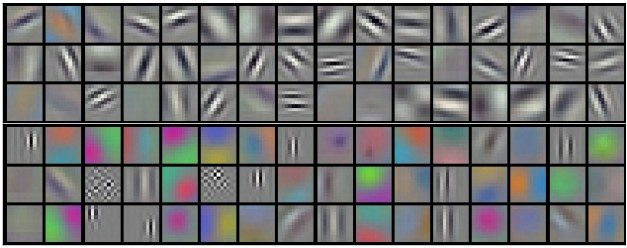
\includegraphics[width=0.8\textwidth]{Figures/ObjRecog/weights}
	\caption{Filters learned by the network proposed by Krizhevsky et al. \cite{Krizhevsky2012}. Each of the 96 filters shown is of size $11\times11\times3$. The filters have clearly learned to detect edges of various orientations and they resemble Gabor filters. Image analysis using that kind of filters is thought to be similar to perception in the human visual system \cite{Marvcelja1980}.}
	\label{fig:alexnet_weights}
\end{figure}

Figure \ref{fig:alexnet_weights} shows some sample filter modules automatically learned by training one of the most successful deep learning architectures: the deep convolutional neural network proposed by Krizhevsky et al. \cite{Krizhevsky2012} to classify the \num{1.2} million high-resolution images in the ImageNet LSVRC-2010 \cite{Berg2010} contest into \num{1000} different classes.

\begin{figure}[!b]
	\centering
    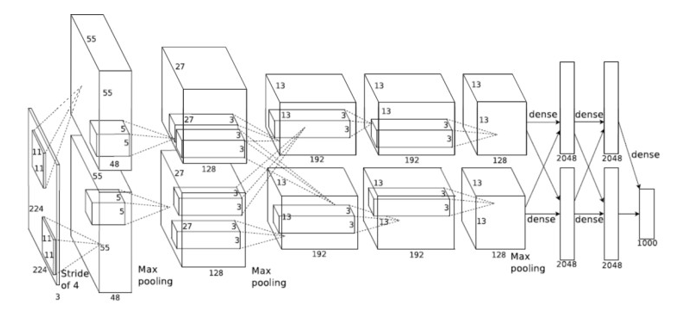
\includegraphics[width=\linewidth]{Figures/ObjRecog/alexnet}
	\caption{Illustration of the architecture of the aforementioned \acs{CNN} proposed by Krizhevsky et al.\cite{Krizhevsky2012} for the ImageNet challenge. Besides the normal components, e.g., convolutional, pooling, and fully connected layers, this network features two different paths. One \ac{GPU} runs the layers at the top while the other runs the layers at the bottom.}
	\label{fig:convnet_architecture}
\end{figure}

In spite of the fact that these kind of architectures showed a huge potential for solving many computer vision problems, they were ignored by the computer vision community. In the latter years, certain breakthrough works revived the interest in deep learning architectures \cite{Lecun2015}. Recent studies proved that local minima are not an issue with large neural networks. Following a set of seminal works for the field on training deep learning networks \cite{Hinton2006}\cite{Bengio2007}, a group of researchers from the \ac{CIFAR} introduced unsupervised learning procedures to create layers of feature detectors without labelled data, they also pre-trained several layers and added a final layer of output units; the system was tuned using backpropagation and achieved a remarkable performance when applied to the handwritten digit recognition or pedestrian detection problems \cite{Sermanet2013}. In addition, the advent of \acp{GPU}, which were easily programmable and extremely efficient for parallel problems, made possible the training of huge networks in acceptable time spans \cite{Raina2009}.

All those contributions to the field led to the birth of probably the most important milestone regarding deep learning: the \acf{CNN}. This special kind of deep network was designed to process data in form of multiple arrays and gained popularity because of its many practical successes. This was due to the fact that they were easier to train and generalized far better than previous models. The architecture of a typical \ac{CNN} is composed by many stages of convolutional layers followed by pooling ones and non-linearity \ac{ReLU} filters; in the end, convolutional and fully connected layers are stacked. The key idea behind using this stack of layers is to exploit the property that many natural signals are compositional hierarchies, in which higher-level features are obtained by composing lower-level ones. Figure \ref{fig:convnet_architecture} shows a typical architecture of a \ac{CNN}.

\subsection{Volumetric Representations}
\label{cha:objrecog:sec:relatedworks:subsec:representations}

Most of the literature focuses on how \acp{CNN} can learn filters and recognize objects using \acs{2D} images as input. In this chapter, we will explore the usage of \acs{3D} information to feed the network. For this purpose, we need volumetric representations for such information. Arguably, the most popular representations for volumetric data are \acs{3D} meshes or point clouds, shown in Figure \ref{subfig:objrecog:3d_mesh_cloud_grid:mesh} and \ref{subfig:objrecog:3d_mesh_cloud_grid:cloud} respectively. A mesh consists of a collection of vertices (points in a \ac{3D} coordinate system), edges (connections between those vertices), and faces (closed sets of edges, usually triangles) that defines the shape of an object. A point cloud is just a set of points defined by $x$, $y$, and $z$ coordinates in a \acl{3D} coordinate system that model the surface of an object. However, those representations are unbounded and barely structured since they contain an arbitrary number of components, e.g., vertices or points, and no particular ordering is enforced for those entities.

\begin{figure}[!t]
	\centering
	\begin{subfigure}{0.2\linewidth}
		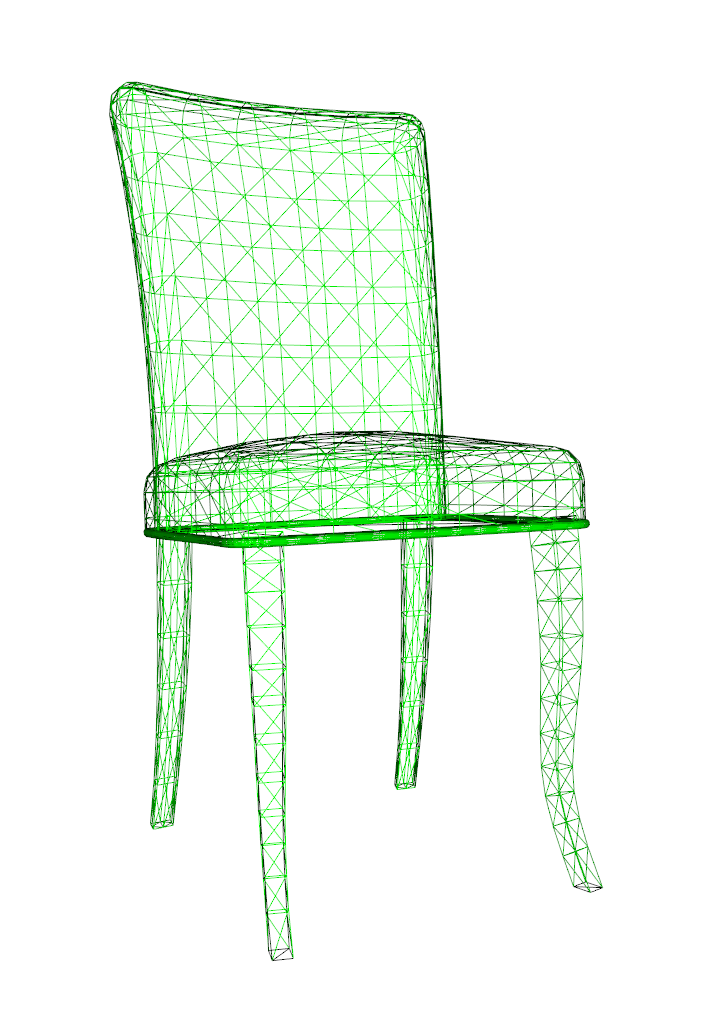
\includegraphics[width=\linewidth]{Figures/ObjRecog/chair_mesh}
		\caption{Mesh}
		\label{subfig:objrecog:3d_mesh_cloud_grid:mesh}
	\end{subfigure}
	\hfill
	\begin{subfigure}{0.2\linewidth}
		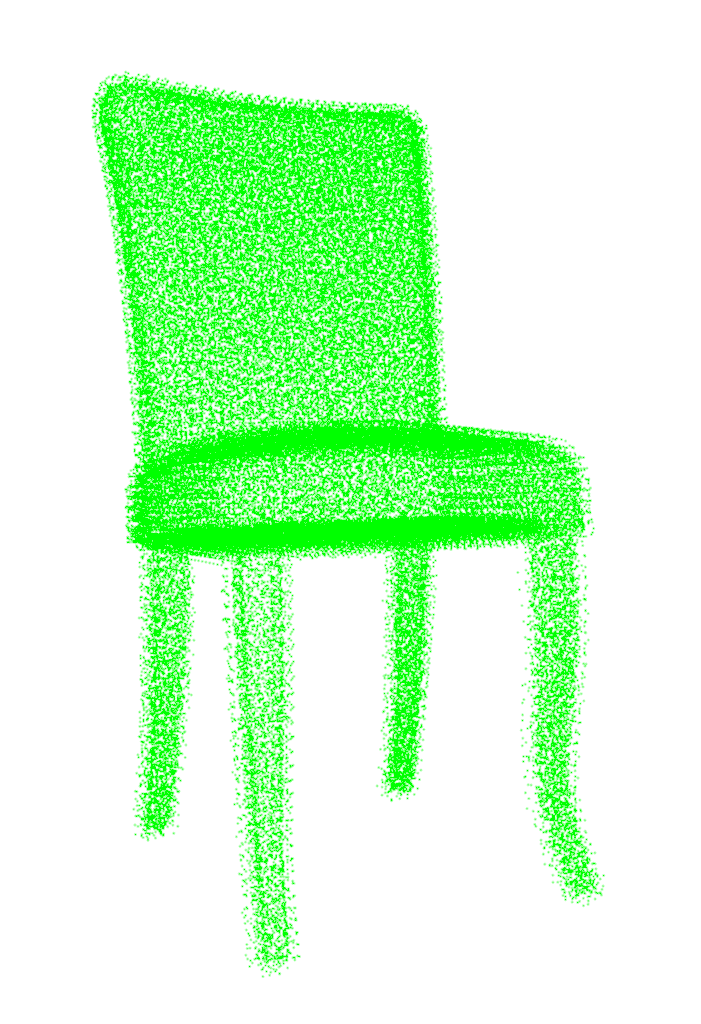
\includegraphics[width=\linewidth]{Figures/ObjRecog/chair_cloud}
		\caption{Point cloud}
		\label{subfig:objrecog:3d_mesh_cloud_grid:cloud}
	\end{subfigure}
	\hfill
	\begin{subfigure}{0.2\linewidth}
		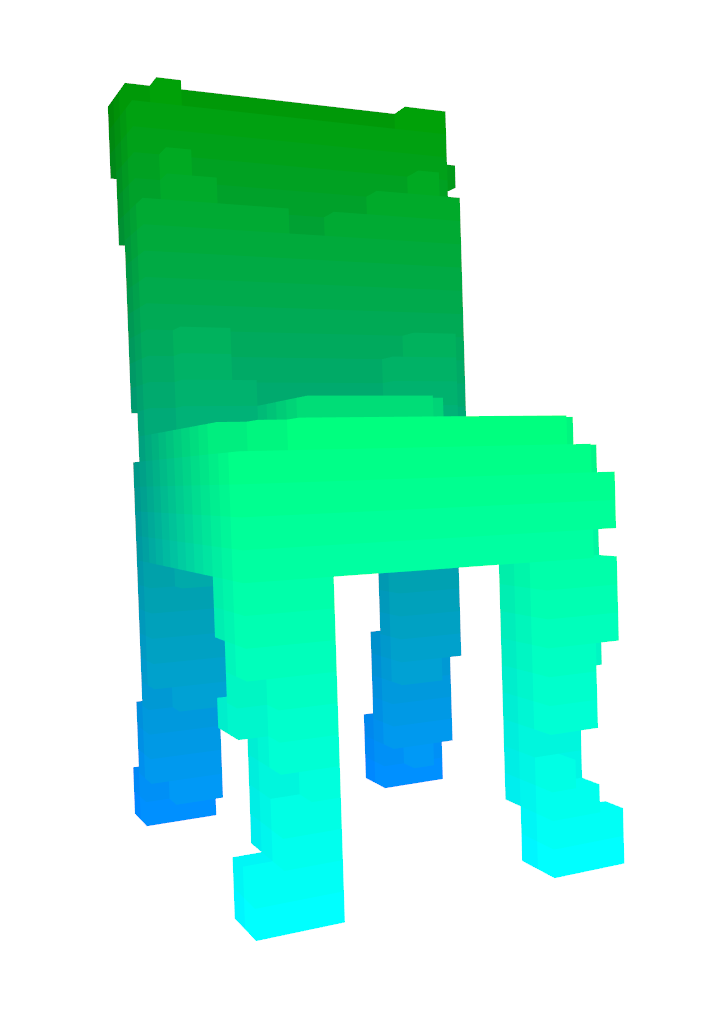
\includegraphics[width=\linewidth]{Figures/ObjRecog/chair_voxel}
		\caption{Voxel grid}
		\label{subfig:objrecog:3d_mesh_cloud_grid:grid}
	\end{subfigure}
	\caption{Common volumetric representations: polygonal mesh (\subref{subfig:objrecog:3d_mesh_cloud_grid:mesh}), point cloud (\subref{subfig:objrecog:3d_mesh_cloud_grid:cloud}), and voxel grid (\subref{subfig:objrecog:3d_mesh_cloud_grid:grid}) of a chair model (which is color coded by height and depth).}
	\label{fig:objrecog:3d_mesh_cloud_grid}
\end{figure}

This fact poses a problem since \acp{CNN} require a fixed-size representation for the input data. In order to overcome this limitation, alternative volumetric representations must be used to provide samples to the network for both training and testing. The most common volumetric representation which allows a structured and bounded definition of an object shape is the voxel grid. A voxel (word contraction of \emph{volume element} or \emph{volumetric pixel}) is the \acs{3D} equivalent to a \acs{2D} pixel, i.e., it is the minimal unit of a \acl{3D} matrix. A volumetric object can be represented as a \ac{3D} matrix of voxels, whose positions are relative to other voxels while points and polygons must be represented explicitly by \ac{3D} coordinates. In this regard, voxels are able to efficiently represent regularly sampled \acs{3D} spaces that are also non-homogeneously filled, while meshes and point clouds are good for representing \acs{3D} shapes with empty or homogeneously filled space. It is important to notice that a voxel is just a data point in a \acl{3D} grid, so its value may represent many different properties. The most popular and simple voxel grid type is the binary one (see Figure \ref{subfig:objrecog:3d_mesh_cloud_grid:grid}) in which each voxel contains a binary value depending on whether the object's surface intersects or is partially contained in the voxel's volume.

\begin{figure}[!t]
	\centering
	\begin{subfigure}{0.32\linewidth}
		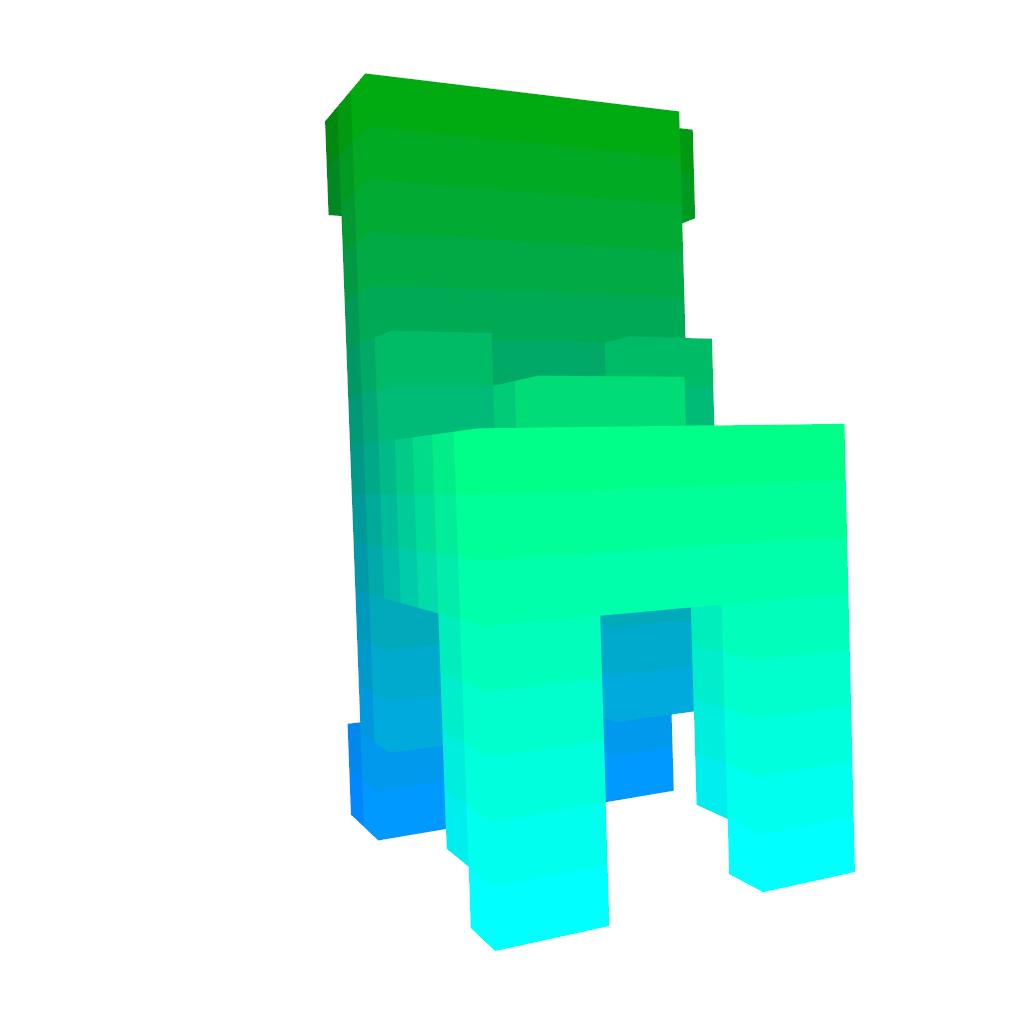
\includegraphics[width=\linewidth]{Figures/ObjRecog/chair_voxel_15}
		\caption{$15\times15\times15$}
		\label{subfig:objrecog:binary_voxel_grids:15}
	\end{subfigure}
	\hfill
	\begin{subfigure}{0.32\linewidth}
		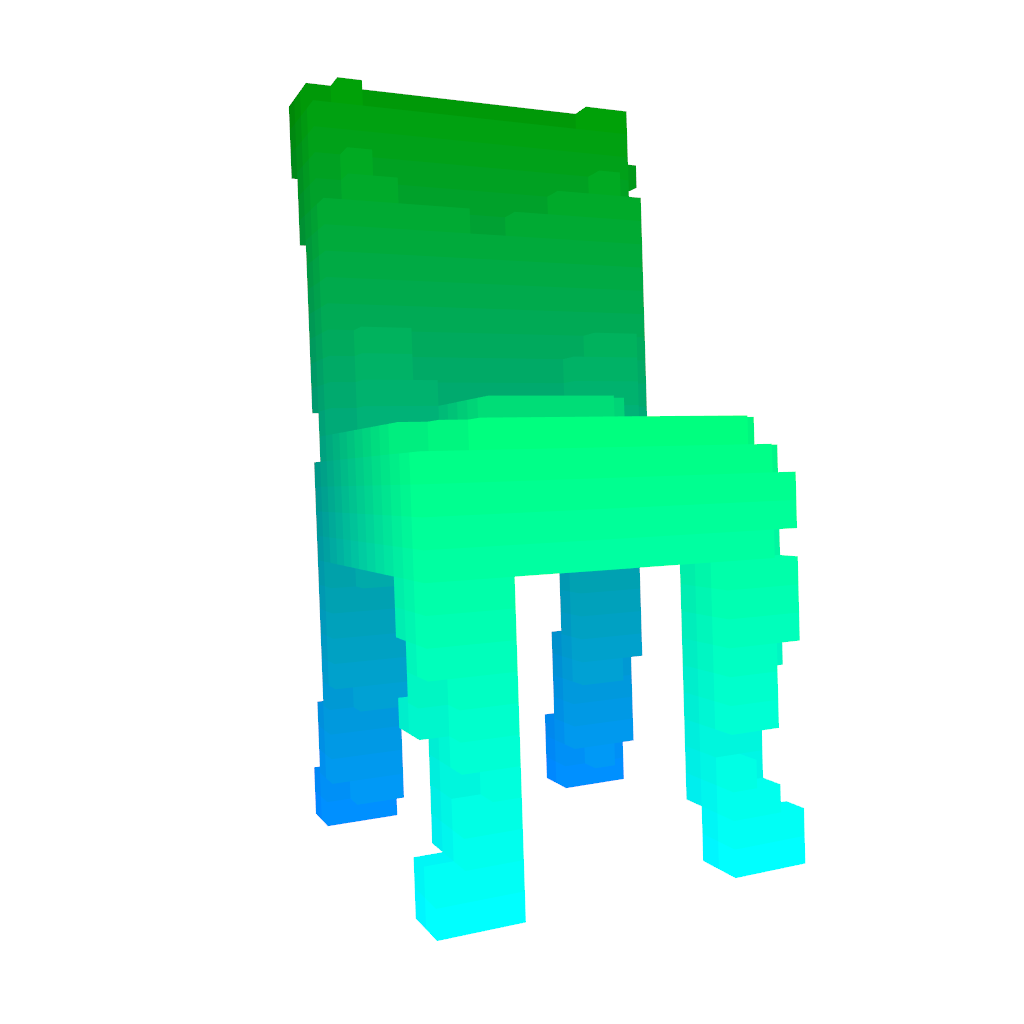
\includegraphics[width=\linewidth]{Figures/ObjRecog/chair_voxel_30}
		\caption{$30\times30\times30$}
		\label{subfig:objrecog:binary_voxel_grids:30}
	\end{subfigure}
	\hfill
	\begin{subfigure}{0.32\linewidth}
		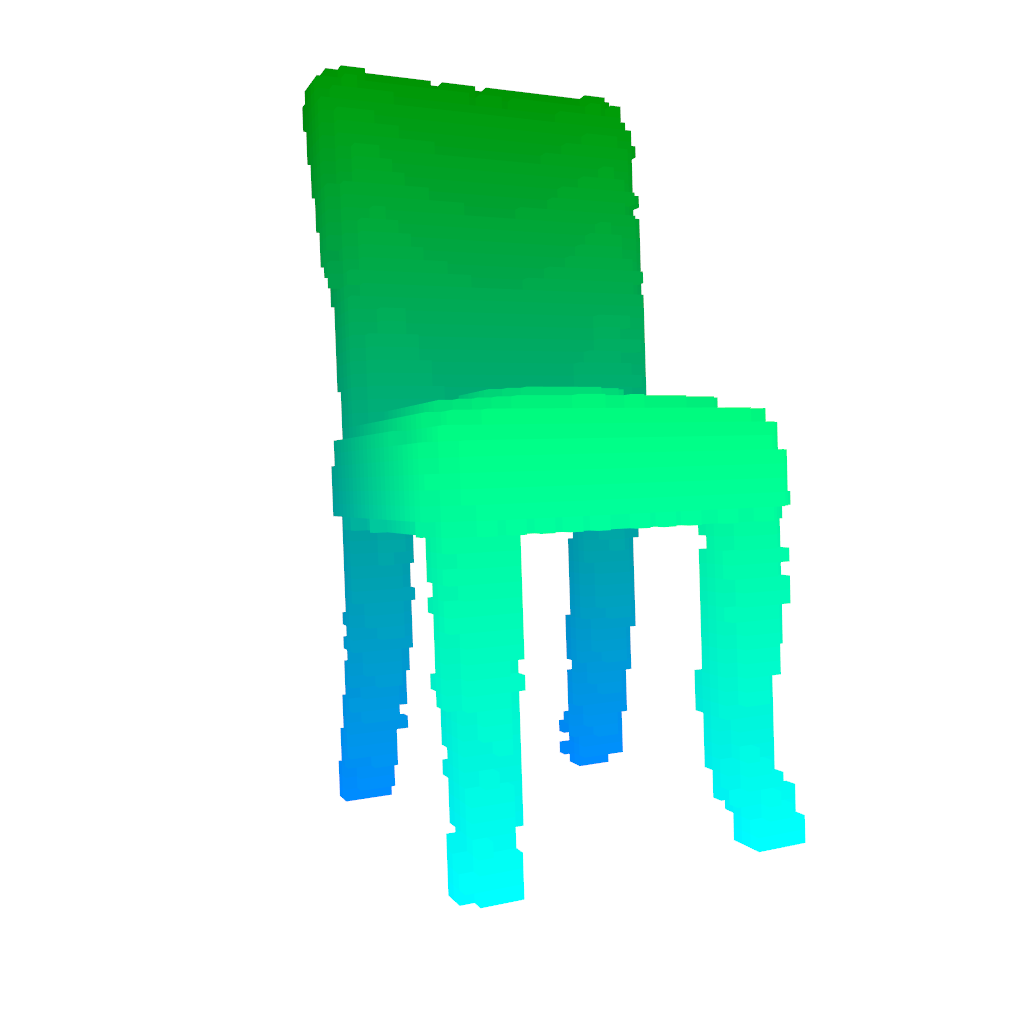
\includegraphics[width=\linewidth]{Figures/ObjRecog/chair_voxel_60}
		\caption{$60\times60\times60$}
		\label{subfig:objrecog:binary_voxel_grids:60}
	\end{subfigure}
	\caption{Effect of the leaf size on binary voxel grids. All grids have the same cubic size: $300\times300\times300$ units. Leaf sizes vary from $5$, $10$, and $20$ units, resulting in binary grids of $15\times15\times15$ (\subref{subfig:objrecog:binary_voxel_grids:15}), $30\times30\times30$ (\subref{subfig:objrecog:binary_voxel_grids:30}), and $60\times60\times60$ voxels (\subref{subfig:objrecog:binary_voxel_grids:60}) respectively.}
	\label{fig:objrecog:binary_voxel_grids}
\end{figure}

Despite the fact that a binary voxel grid representation allows us to feed a \ac{CNN} with volumetric data coming from different sources (point clouds provided by range sensors or polygonal meshes from \acs{3D} models can be easily converted into voxel grids) a significant amount of information from the original representation is lost. This loss depends on the resolution of the grid, i.e., the voxel size which is usually referred as the \emph{leaf size}. Figure \ref{fig:objrecog:binary_voxel_grids} shows how the resolution of the voxel grid can be tuned to obtain more accurate or more compact volumetric representations. Although an arbitrary precision can be obtained by changing the leaf size, it is hard to determine a specific size which describes with enough detail all the possible inputs for the \ac{CNN} without sacrificing the compactness of the grid. 

Apart from those basic representations, others which maintain the properties of the voxel grid, but include additional information in the values of the cells can be used as well. Here we briefly review the most popular and successful volumetric representations for \acs{3D} data that have been used to feed \acp{CNN} for object recognition purposes.

\begin{figure}[!b]
	\centering
	\hfill
	\begin{subfigure}{0.32\textwidth}
		\centering
		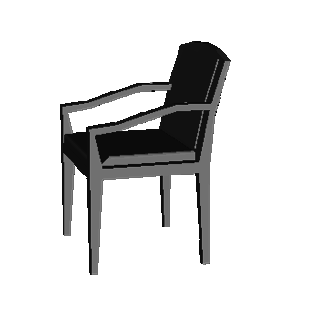
\includegraphics[width=\linewidth]{Figures/ObjRecog/chair_model}
		\caption{Object model}
		\label{subfig:objrecog:3dshapenets:model}
	\end{subfigure}
	\hfill
	\begin{subfigure}{0.32\textwidth}
		\centering
		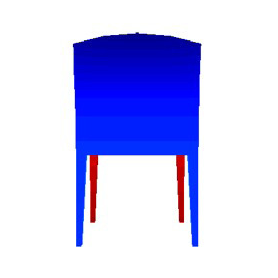
\includegraphics[width=\linewidth]{Figures/ObjRecog/chair_view}
		\caption{Depth map}
		\label{subfig:objrecog:3dshapenets:depth}
	\end{subfigure}
	\hfill
	\begin{subfigure}{0.32\textwidth}
		\centering
		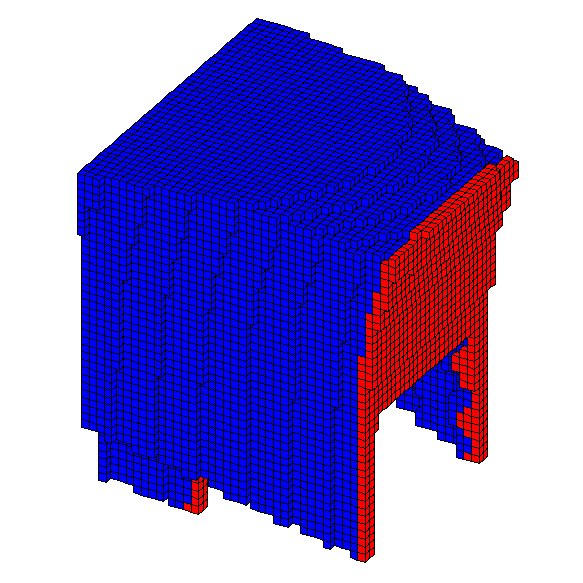
\includegraphics[width=\linewidth]{Figures/ObjRecog/chair_grid_occluded}
		\caption{Voxel grid}
		\label{subfig:objrecog:3dshapenets:grid}
	\end{subfigure}
	\hfill
	\caption{\emph{3DShapeNets} representation proposed by Wu \emph{et al.} as shown in their paper \cite{Wu2015}. An object (\subref{subfig:objrecog:3dshapenets:model}) is captured from a certain point of view and a depth map is generated (\subref{subfig:objrecog:3dshapenets:depth}) which is in turn used to generate a point cloud that will be represented as a voxel grid (\subref{subfig:objrecog:3dshapenets:grid}) with empty voxels (in white, not represented), unknown voxels (in blue), and surface or occupied voxels (red).}
	\label{fig:objrecog:3dshapenets}
\end{figure}

The first step was taken by Wu \emph{et al.} \cite{Wu2015}; their work \emph{3DShapeNets} was the first to apply \acp{CNN} to pure \acs{3D} representations. Their proposal (shown in Figure \ref{fig:objrecog:3dshapenets}) represents \acs{3D} shapes, from captured depth maps that are later transformed into point clouds, as \acs{3D} voxel grids of size $30\times30\times30$ voxels -- $24\times24\times24$ data voxels plus $3$ extra ones of padding in both directions to reduce convolution artifacts -- which can represent free space, occupied space (the shape itself), and unknown or occluded space depending on the point of view. Neither the grid generation process, nor the leaf size is described but the voxel grid relies on prior object segmentation.

Song and Xiao \cite{Song2015} proposed to adopt a directional \ac{TSDF} encoding which takes a depth map as input and outputs a volumetric representation. They divide a \acs{3D} space using an equally spaced voxel grid in which each cell holds a \acl{3D} vector that records the shortest distance between the voxel center and the \acl{3D} surface in three directions. In addition, the value is clipped by $2\delta$, being $\delta$ the grid size in each dimension. A $30\times30\times30$ voxels grid is fitted to a previously segmented object candidate. Figure \ref{fig:objrecog:tsdf} shows a graphical representation of this approach.

\begin{figure}[!t]
	\centering
	\hfill
	\begin{subfigure}{0.26\textwidth}
		\centering
		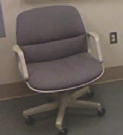
\includegraphics[width=\linewidth]{Figures/ObjRecog/song_chair_rgb}
		\caption{Object}
		\label{subfig:objrecog:tsdf:object}
	\end{subfigure}
	\hfill
	\begin{subfigure}{0.22\textwidth}
		\centering
		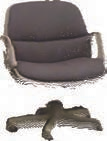
\includegraphics[width=\linewidth]{Figures/ObjRecog/song_chair_cloud}
		\caption{Point cloud}
		\label{subfig:objrecog:tsdf:cloud}
	\end{subfigure}
	\hfill
	\begin{subfigure}{0.3\textwidth}
		\centering
		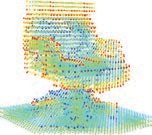
\includegraphics[width=\linewidth]{Figures/ObjRecog/song_chair_tsdf}
		\caption{\ac{TSDF} grid}
		\label{subfig:objrecog:tsdf:grid}
	\end{subfigure}
	\hfill
	\caption{\ac{TSDF} representation proposed by Song and Xiao as shown in their paper \cite{Song2015}. An object (\subref{subfig:objrecog:tsdf:object}) is captured by a range sensor as a point cloud (\subref{subfig:objrecog:tsdf:cloud}) and then a \ac{TSDF} grid is generated (red indicates the voxel is in front of surfaces and blue indicates the voxel is behind the surface; the intensity of the color represents the \acs{TSDF} value).}
	\label{fig:objrecog:tsdf}
\end{figure}

\begin{figure}[!b]
	\centering
	\hfill
	\begin{subfigure}{0.23\textwidth}
		\centering
		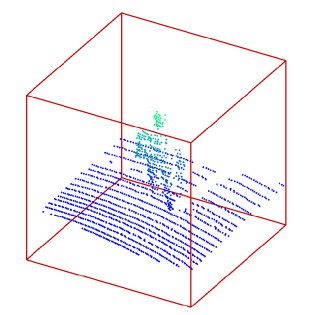
\includegraphics[width=\linewidth]{Figures/ObjRecog/voxnet_1}
		\caption{\acs{LIDAR} data}
		\label{subfig:objrecog:voxnet:lidar}
	\end{subfigure}
	\hfill
	\begin{subfigure}{0.23\textwidth}
		\centering
		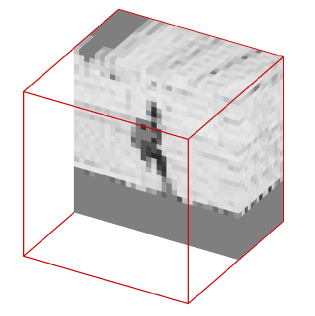
\includegraphics[width=\linewidth]{Figures/ObjRecog/voxnet_4}
		\caption{Voxnet grid}
		\label{subfig:objrecog:voxnet:lidar_grid}
	\end{subfigure}
	\hfill
	\begin{subfigure}{0.23\textwidth}
		\centering
		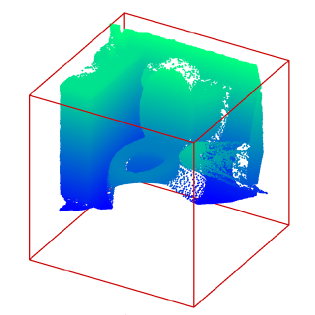
\includegraphics[width=\linewidth]{Figures/ObjRecog/voxnet_2}
		\caption{RGBD data}
		\label{subfig:objrecog:voxnet:rgbd}
	\end{subfigure}
	\hfill
	\begin{subfigure}{0.23\textwidth}
		\centering
		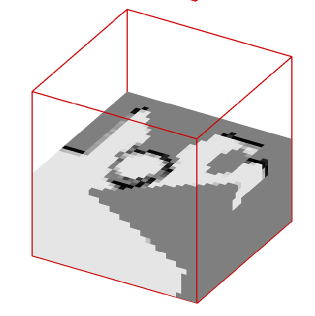
\includegraphics[width=\linewidth]{Figures/ObjRecog/voxnet_3}
		\caption{Voxnet grid}
		\label{subfig:objrecog:voxnet:rgbd_grid}
	\end{subfigure}
	\hfill
	\caption{Volumetric occupancy grid representation used by \emph{VoxNet} as shown in their paper \cite{Maturana2015}. For \acs{LIDAR} data (\subref{subfig:objrecog:voxnet:lidar}) a voxel size of $0.1$m$^3$ is used to create a $32\times32\times32$ grid (\subref{subfig:objrecog:voxnet:lidar_grid}). For \acs{RGB-D} data (\subref{subfig:objrecog:voxnet:rgbd}), the resolution is chosen so the object occupies a subvolume of $24\times24\times24$ voxels in a $32\times32\times32$ grid (\subref{subfig:objrecog:voxnet:rgbd_grid}).}
	\label{fig:objrecog:voxnet}
\end{figure}

Maturana and Scherer \cite{Maturana2015} use occupancy grids in \emph{VoxNet} to maintain a probabilistic estimate of the occupancy of each voxel to represent a \acs{3D} shape. This estimate is a function of the sensor data and prior knowledge. They propose three different occupancy models: binary, density, and hit. The binary and density models make use of raytracing to compute the number of hits and pass-throughs for each voxel. The former one assumes that each voxel has a binary state, occupied or unoccupied. The latter one assumes that each voxel has a continuous density, based on the probability it will block a sensor beam. The hit grid ignores the difference between unknown and free space, only considering hits; it discards information but does not require the use of raytracing so it is highly efficient in comparison with the other methods. They also propose two different grids for \ac{LIDAR} and \acs{RGB-D} sensor data. For the \acs{RGB-D} case, they use a fixed occupancy grid of $32\times32\times32$ voxels, making the object of interest -- obtained by a segmentation algorithm or given by a sliding box -- occupy a subvolume of $24\times24\times24$ voxels. The $z$ axis of the grid is aligned with the direction of gravity. Figure \ref{fig:objrecog:voxnet} shows the occupancy grids used by \emph{VoxNet}.

\subsection{Our Proposal in Context}
\label{cha:objrecog:sec:relatedworks:subsec:context}

Our proposal builds upon the successes in the literature which suggested that applying deep learning techniques to 3D information to solve the object class recognition problem exhibits potential to raise the bar in terms of performance. Firstly, we introduce a novel way for representing the \ac{3D} input data, which is based on point density occupancy grids, and we integrate it into a \ac{CNN} architecture. The focus of this first iteration is to prove that simple representations and architectures for 3D data can perform reasonably well while keeping computational cost at bay to enable real-time class recognition. Secondly, we carry out an in-depth study of the effect of adverse conditions that characterize real-world scenarios -- such as noise caused by the sensor and occlusions due to the positions of the objects in the scene -- on the performance of \acp{CNN} applied to \acs{3D} object class recognition. In this case, our target is the assessment of iterative improvements applied to the previous architecture and representations to show that not only they can perform real-time recognition at reasonable accuracy but also maintain it under adverse circumstances. At last, we take a sideways step to propose a novel approach that uses multiple \ac{2D} cross-section views of \ac{3D} models for \ac{3D} object class recognition.

\section{Datasets}
\label{cha:objrecog:sec:datasets}

Deep neural network architectures are usually composed by many layers which in turn mean many weights to be learned. Because of that, there is a strong need of large-scale datasets to train those networks in order to avoid overfitting the model to the input data. Nowadays, large-scale databases of real-world \acs{3D} objects are scarce, some of them do not have that high number of objects \cite{Lai2011}\cite{Singh2014}\cite{Li2014}, or were incomplete by the time this work was performed \cite{Choi2016}. A possible workaround to this problem consists of using \ac{CAD} model databases -- which are virtually unlimited -- and processing those models to simulate real-world data.

The \emph{Princeton ModelNet} project is one of the most popular large-scale \acs{3D} object dataset. Its goal, as their authors state, is to provide researchers with a comprehensive clean collection of \acs{3D} \ac{CAD} models for objects, which were obtained via online search engines. Employees from the \ac{AMT} service were hired to classify over \num{150000} models into \num{662} different categories.

At the moment, there are two versions of this dataset publicly available for download\footnote{\url{http://modelnet.cs.princeton.edu/}}: \emph{ModelNet-10} and \emph{ModelNet-40}. Those are subsets of the original dataset which only provide the \num{10} and \num{40} most popular object categories respectively. These subsets are specially clean versions of the complete dataset.

On the one hand, ModelNet-10 is composed of a collection of over 5000 models classified into 10 categories and divided into training and test splits. In addition, the orientation of all \ac{CAD} models of the dataset was manually aligned. On the other hand, ModelNet-40 features over \num{9800} models classified into \num{40} categories, also including training and test sets. However, the orientations of its models are not aligned as they are in ModelNet-10. Figure \ref{fig:objrecog:modelnet_models} shows some model examples from ModelNet-10. Figure \ref{fig:objrecog:modelnet_distribution} and Table \ref{table:objrecog:modelnet_distribution} show the model distribution per each class of both subsets taking into account the training and test splits. 

Since the final goal of the \acp{CNN} is to provide means to recognize objects onboard a mobile robotic platform which features \ac{RGB-D} sensors, it is logical to transform the full mesh representation provided by the dataset into the representation that our networks will deal with. \ac{RGB-D} cameras output depth maps which can be used to generate \acs{3D} point clouds of the scene viewed by the camera. In this regard, we will transform each \ac{CAD} object of the dataset into partial point clouds from different \acp{PoV}.

\clearpage

\begin{figure}[!t]
	\centering
	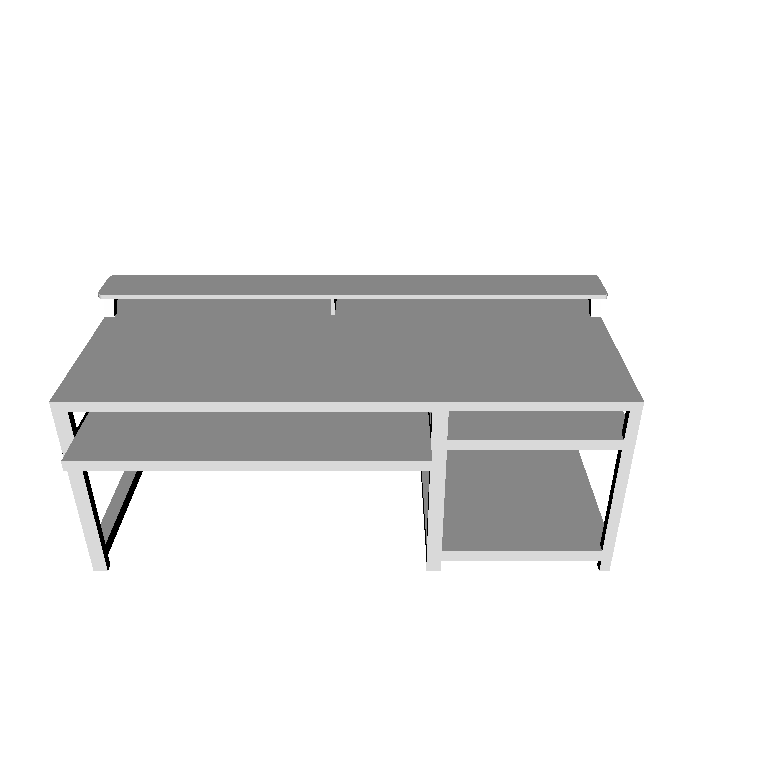
\includegraphics[width=0.15\textwidth]{Figures/ObjRecog/desk_0}\hfill
	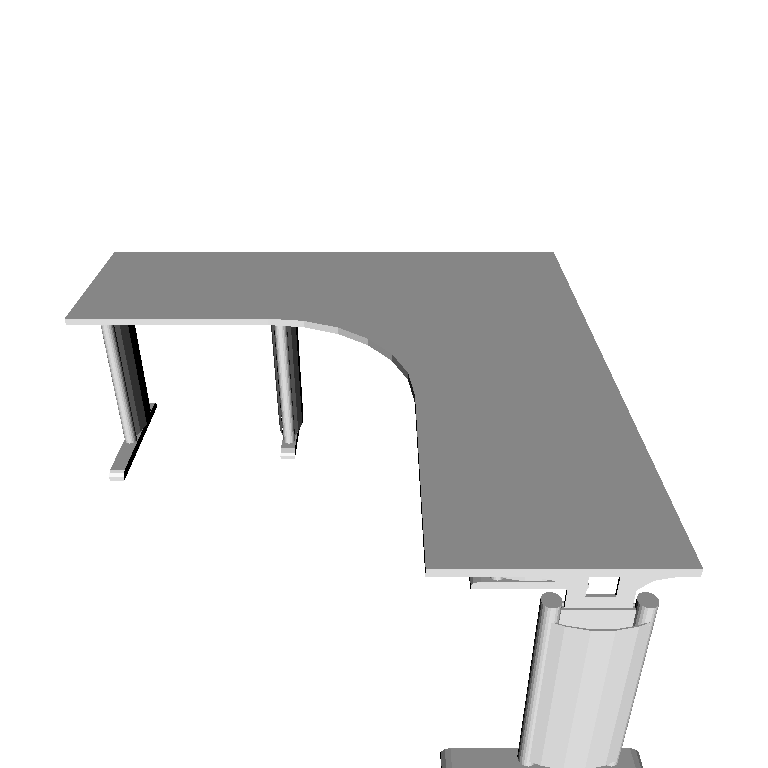
\includegraphics[width=0.15\textwidth]{Figures/ObjRecog/desk_1}\hfill
	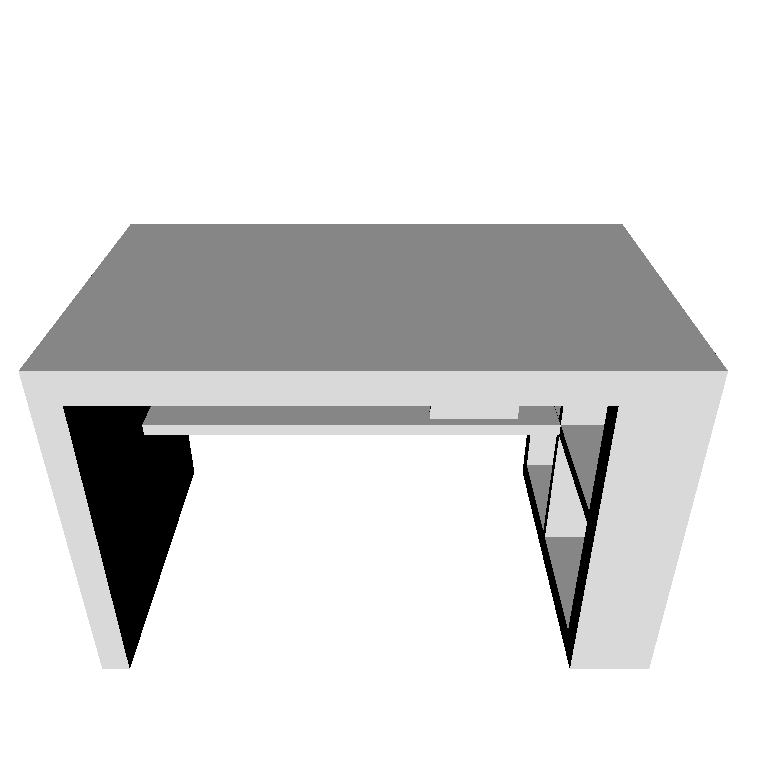
\includegraphics[width=0.15\textwidth]{Figures/ObjRecog/desk_2}\hfill
	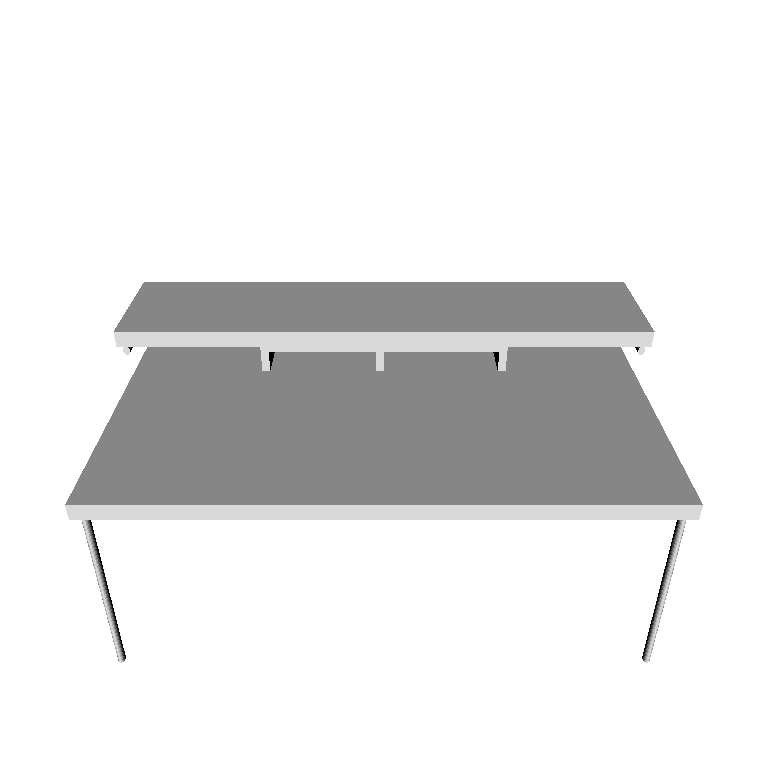
\includegraphics[width=0.15\textwidth]{Figures/ObjRecog/desk_3}\hfill
	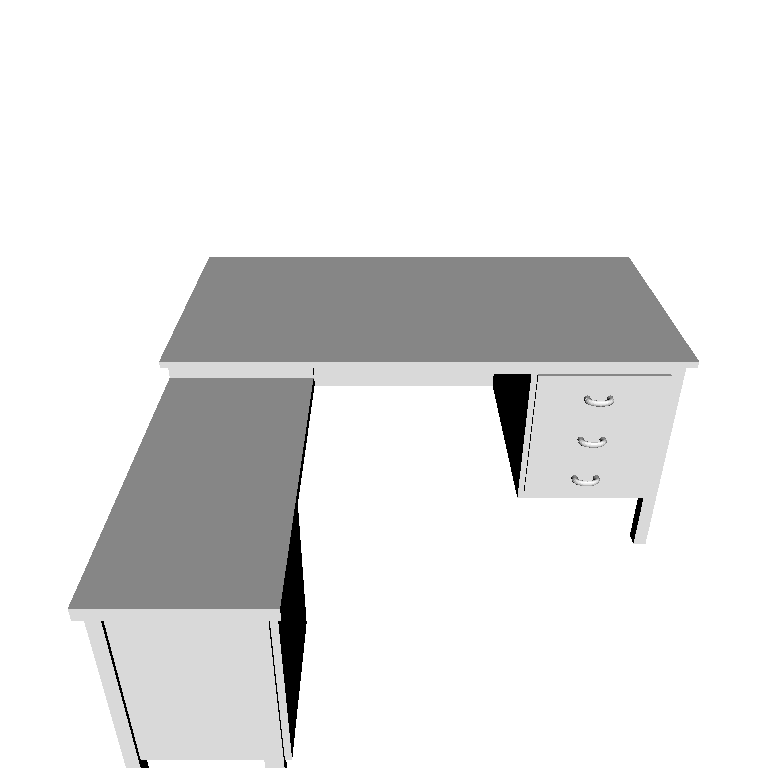
\includegraphics[width=0.15\textwidth]{Figures/ObjRecog/desk_4}\hfill

	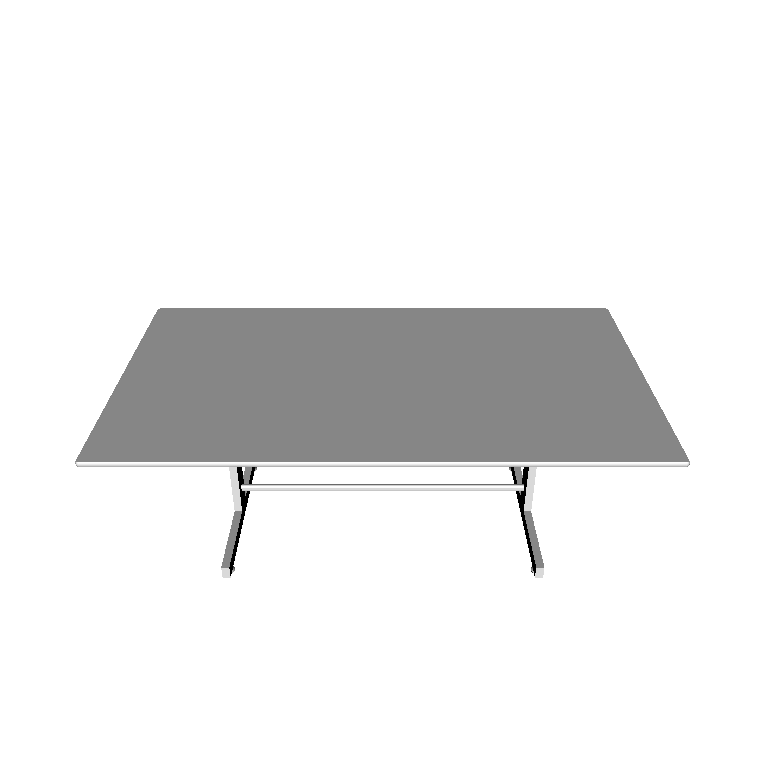
\includegraphics[width=0.15\textwidth]{Figures/ObjRecog/table_0}\hfill
	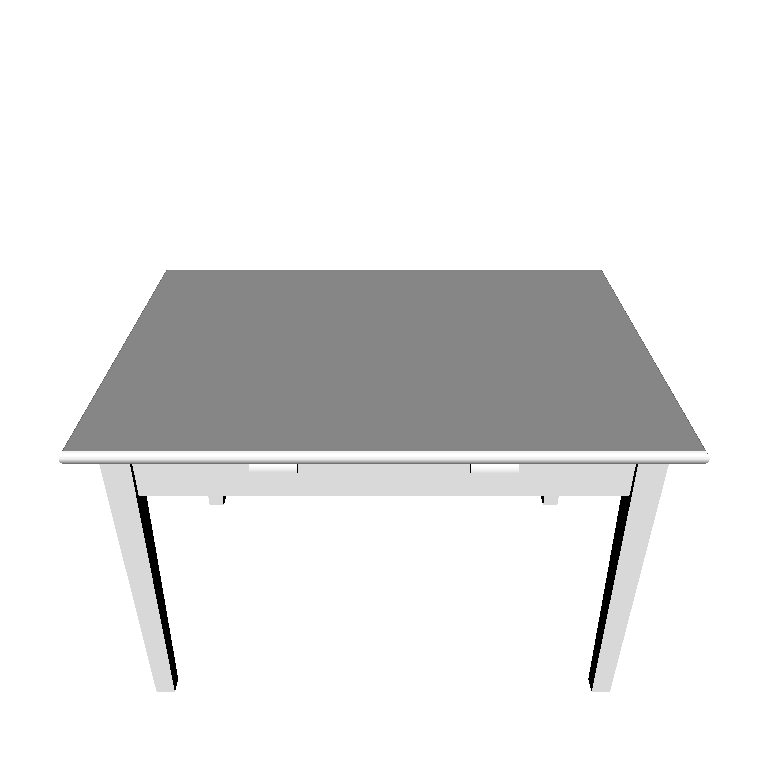
\includegraphics[width=0.15\textwidth]{Figures/ObjRecog/table_1}\hfill
	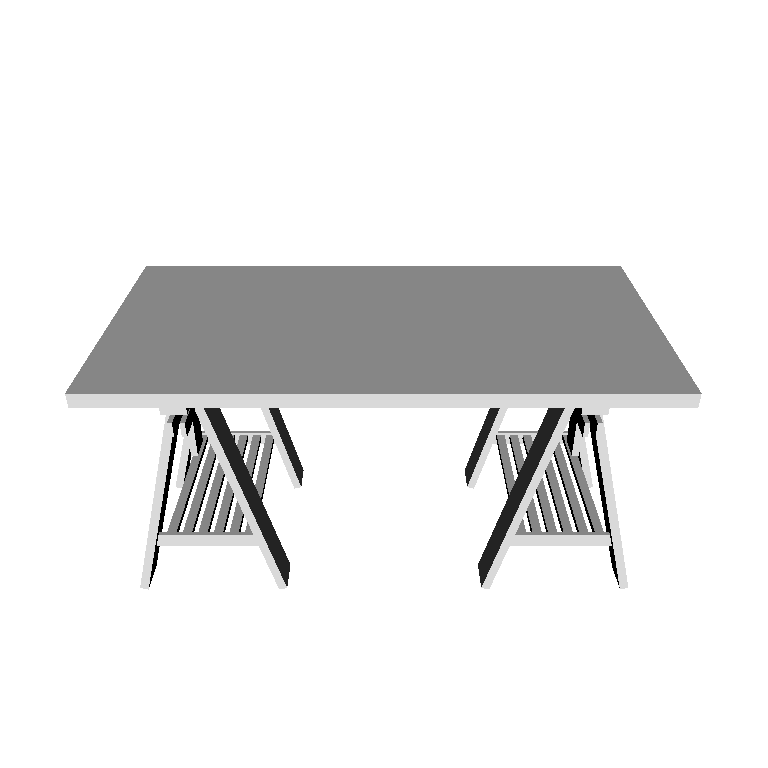
\includegraphics[width=0.15\textwidth]{Figures/ObjRecog/table_2}\hfill
	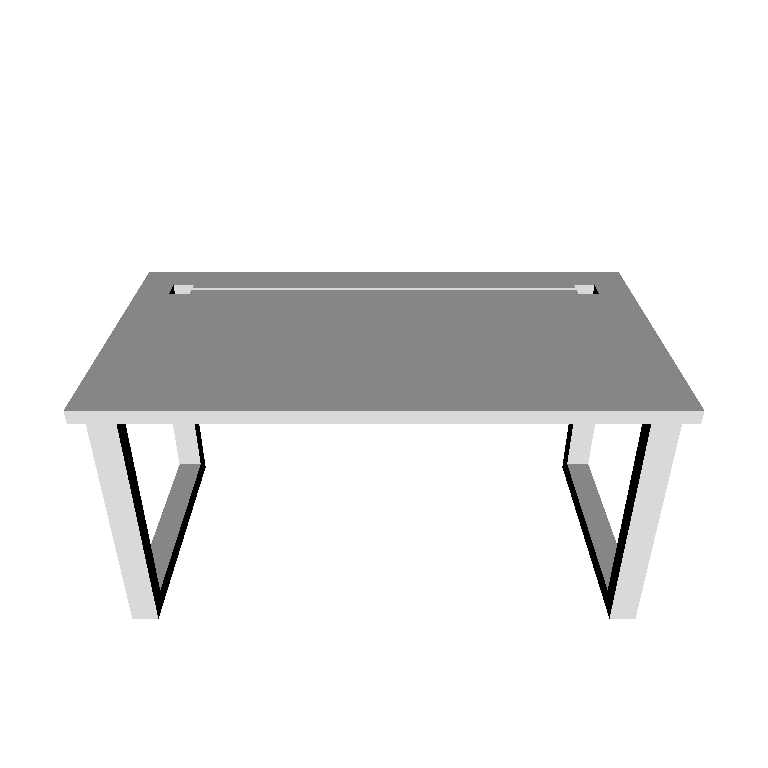
\includegraphics[width=0.15\textwidth]{Figures/ObjRecog/table_3}\hfill
	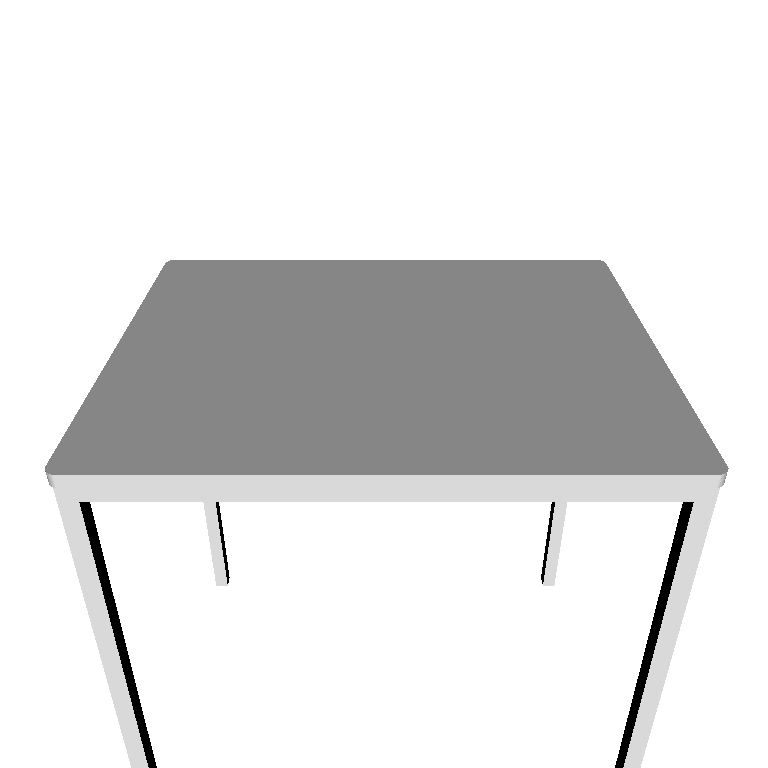
\includegraphics[width=0.15\textwidth]{Figures/ObjRecog/table_4}\hfill

	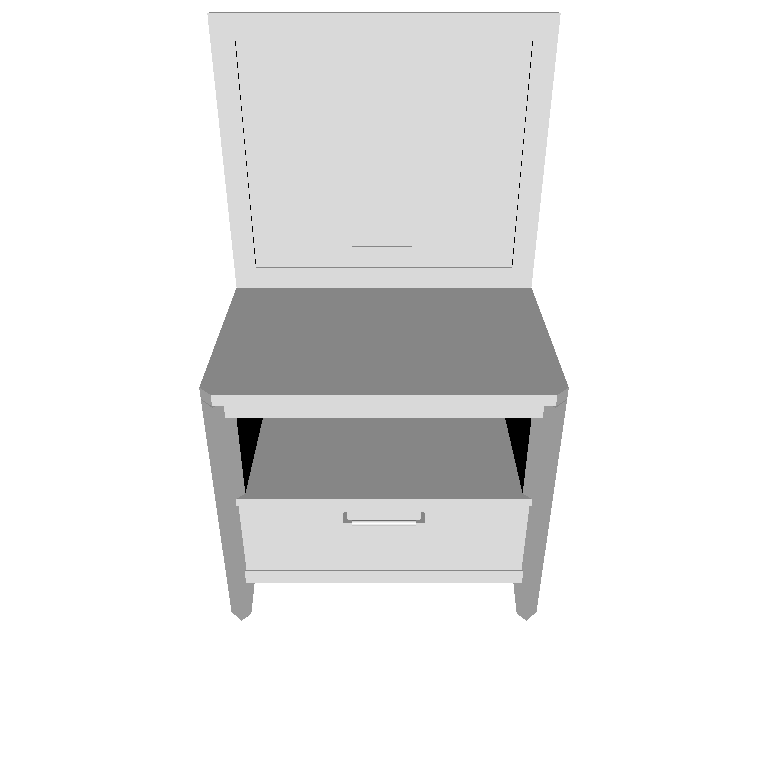
\includegraphics[width=0.15\textwidth]{Figures/ObjRecog/nstand_0}\hfill
	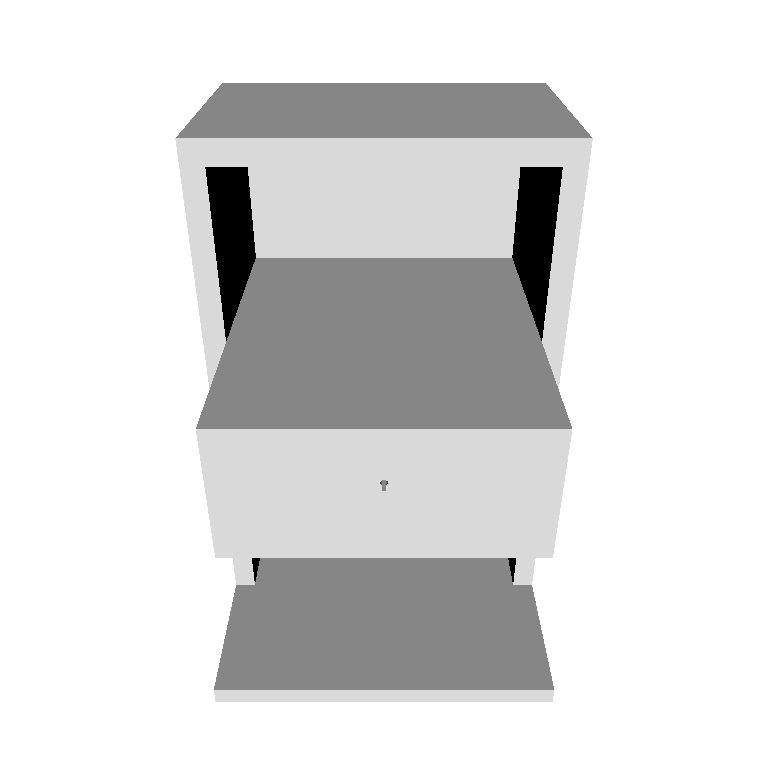
\includegraphics[width=0.15\textwidth]{Figures/ObjRecog/nstand_1}\hfill
	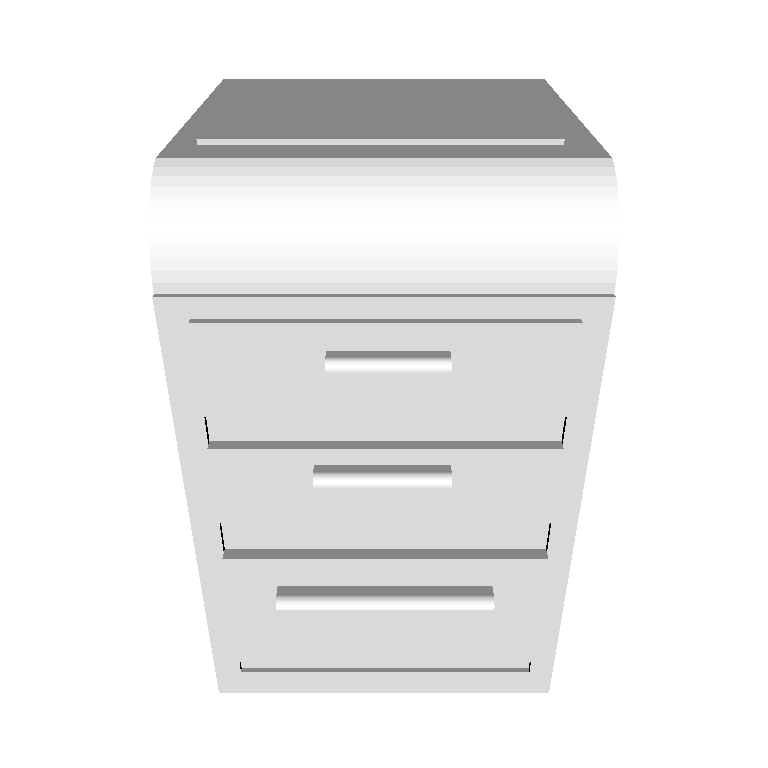
\includegraphics[width=0.15\textwidth]{Figures/ObjRecog/nstand_2}\hfill
	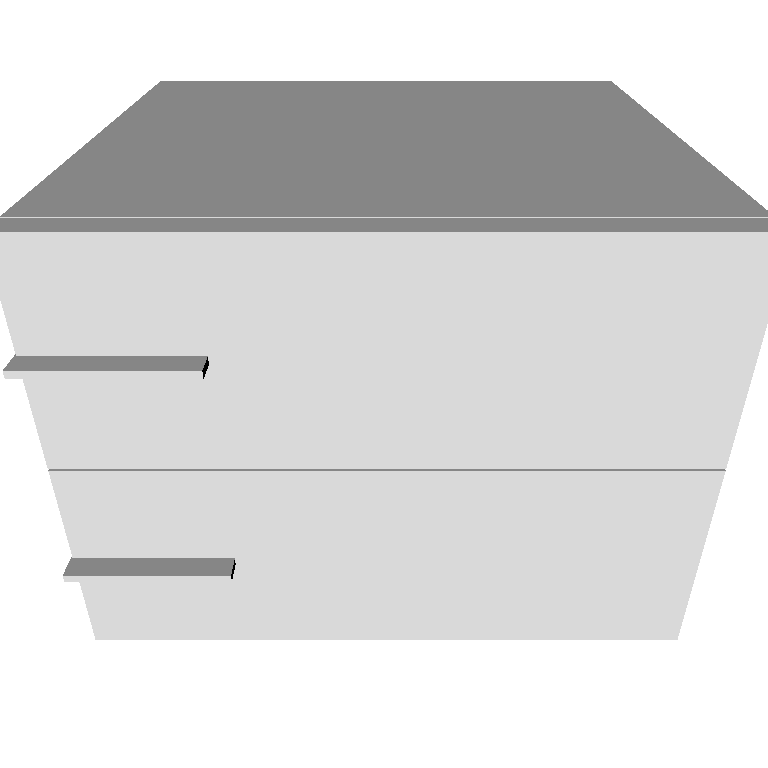
\includegraphics[width=0.15\textwidth]{Figures/ObjRecog/nstand_3}\hfill
	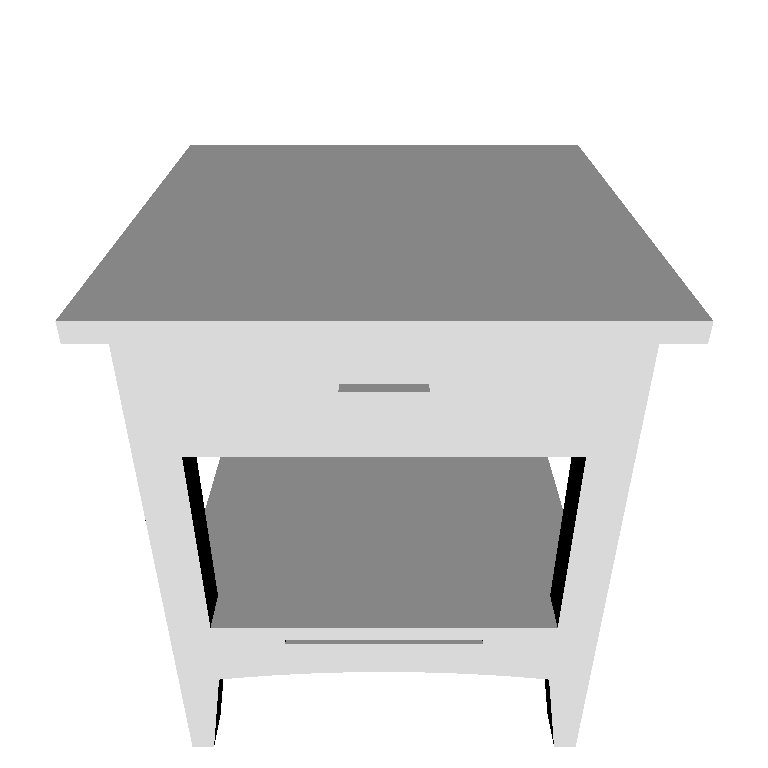
\includegraphics[width=0.15\textwidth]{Figures/ObjRecog/nstand_4}\hfill

	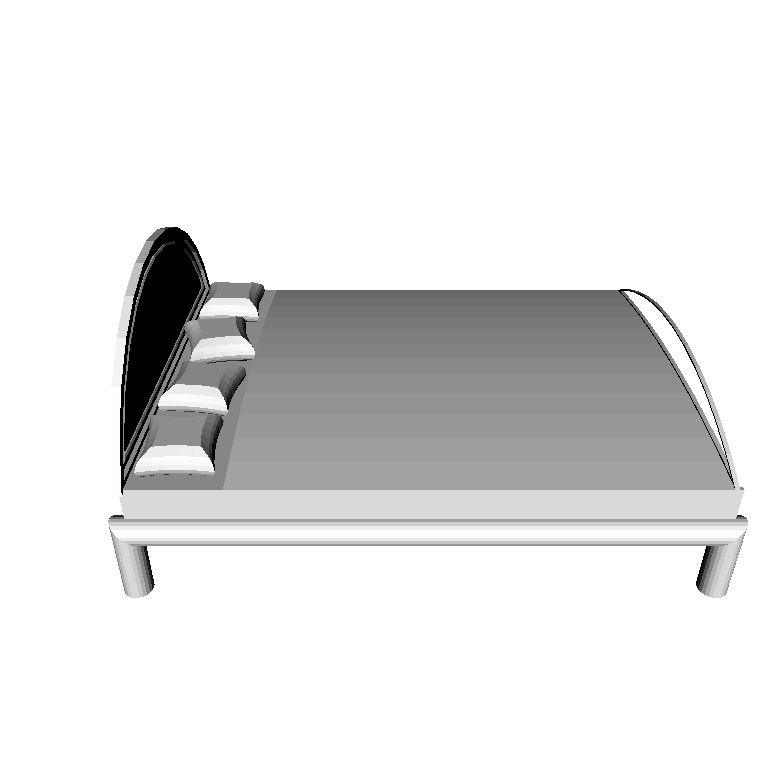
\includegraphics[width=0.15\textwidth]{Figures/ObjRecog/bed_0}\hfill
	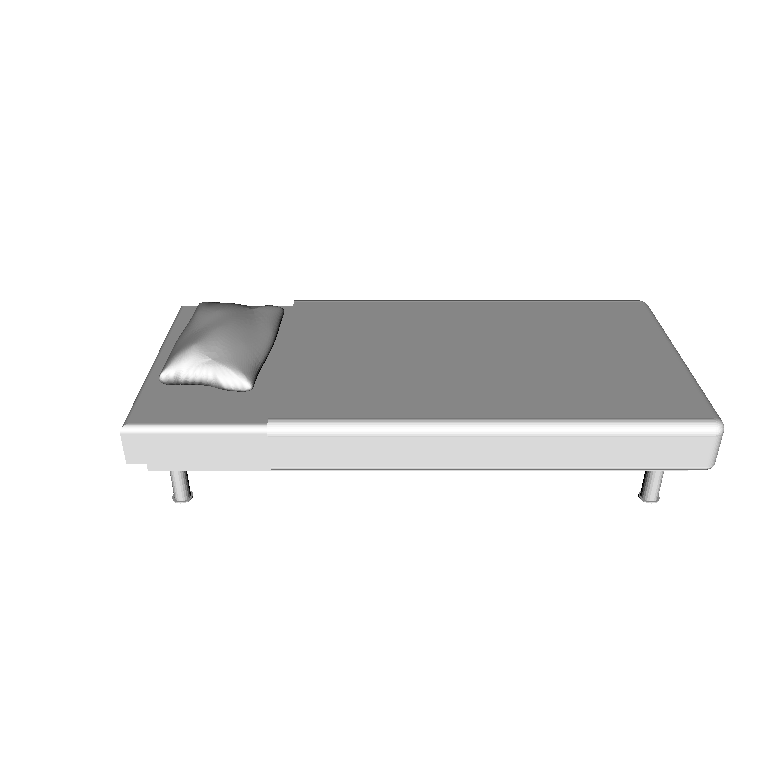
\includegraphics[width=0.15\textwidth]{Figures/ObjRecog/bed_1}\hfill
	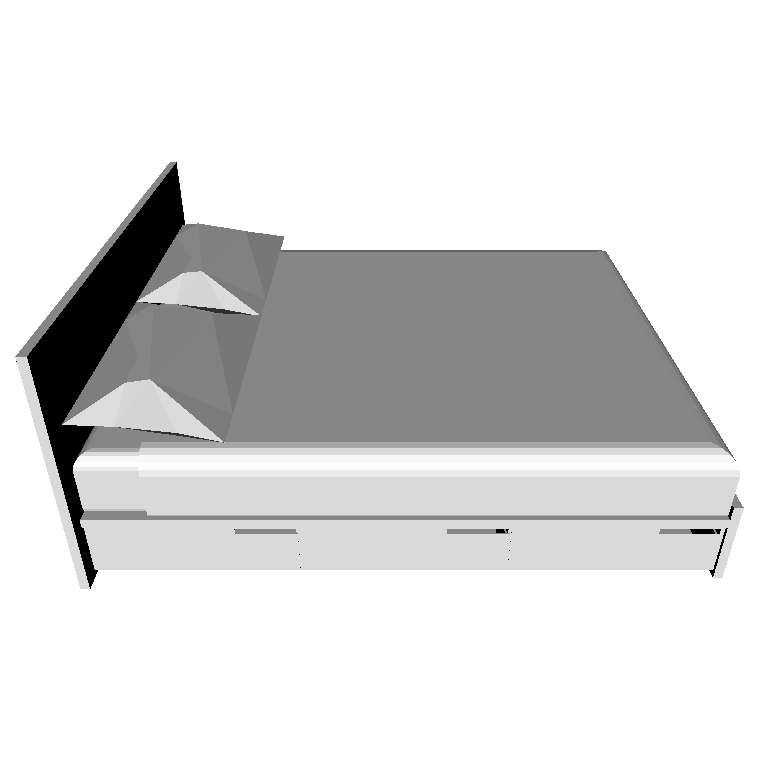
\includegraphics[width=0.15\textwidth]{Figures/ObjRecog/bed_2}\hfill
	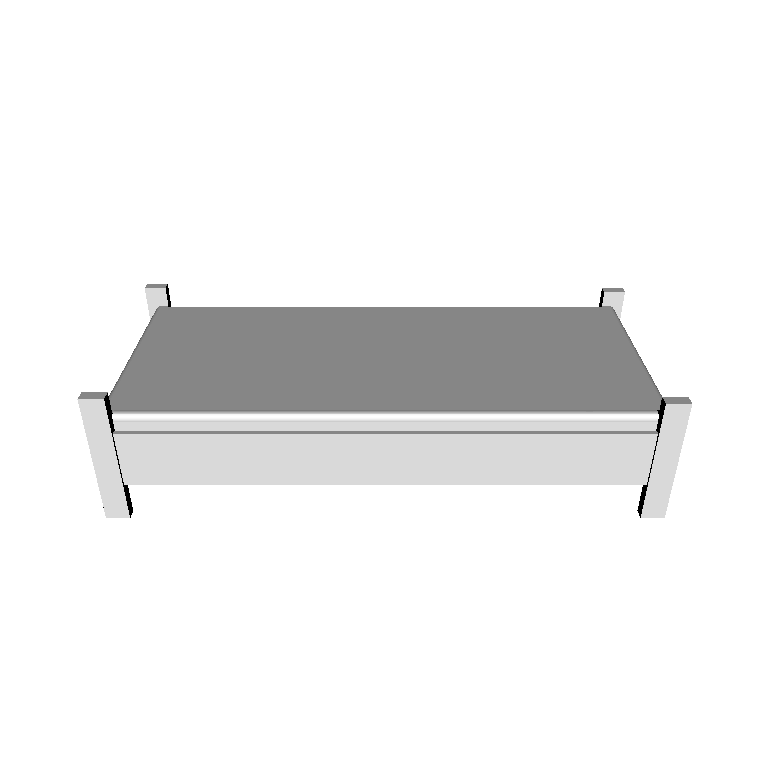
\includegraphics[width=0.15\textwidth]{Figures/ObjRecog/bed_3}\hfill
	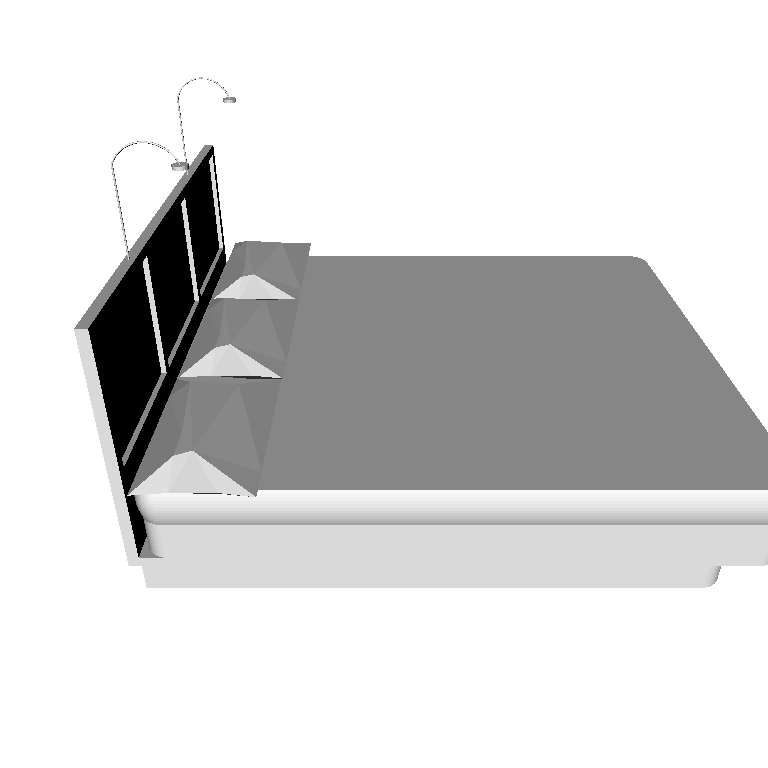
\includegraphics[width=0.15\textwidth]{Figures/ObjRecog/bed_4}\hfill

	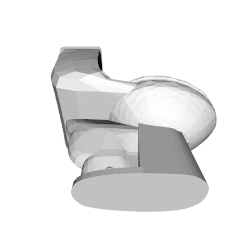
\includegraphics[width=0.15\textwidth]{Figures/ObjRecog/toilet_0}\hfill
	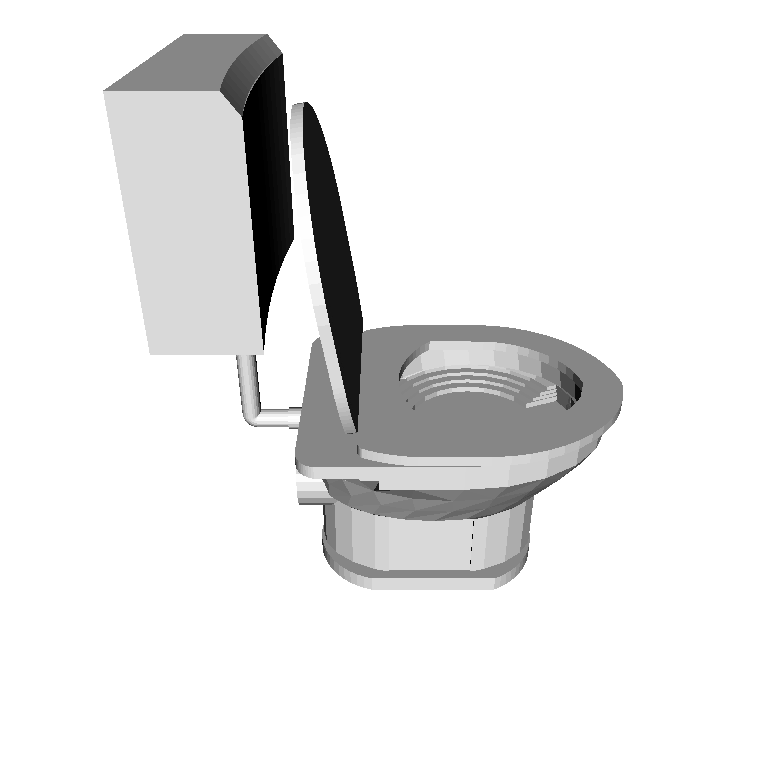
\includegraphics[width=0.15\textwidth]{Figures/ObjRecog/toilet_1}\hfill
	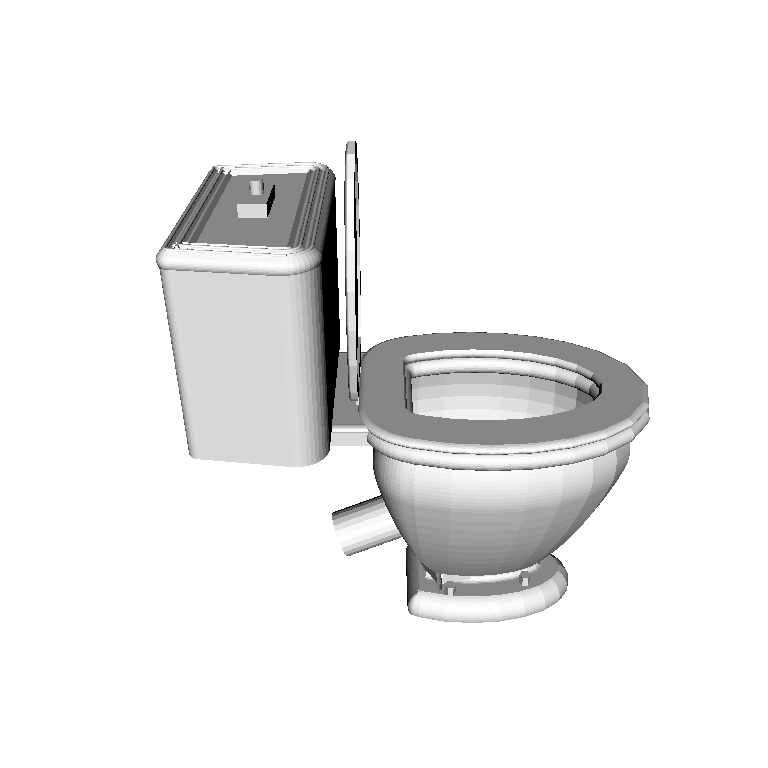
\includegraphics[width=0.15\textwidth]{Figures/ObjRecog/toilet_2}\hfill
	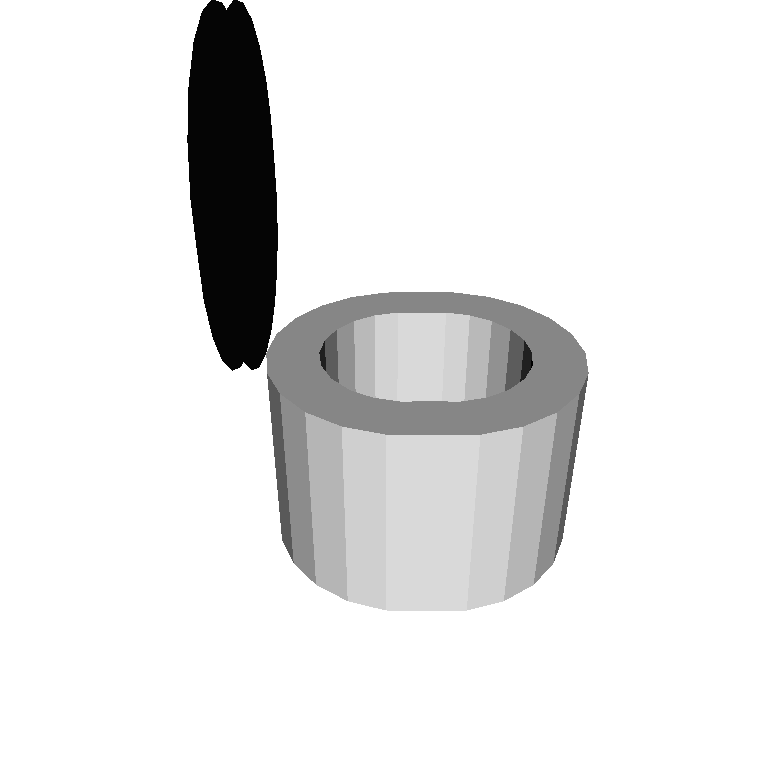
\includegraphics[width=0.15\textwidth]{Figures/ObjRecog/toilet_3}\hfill
	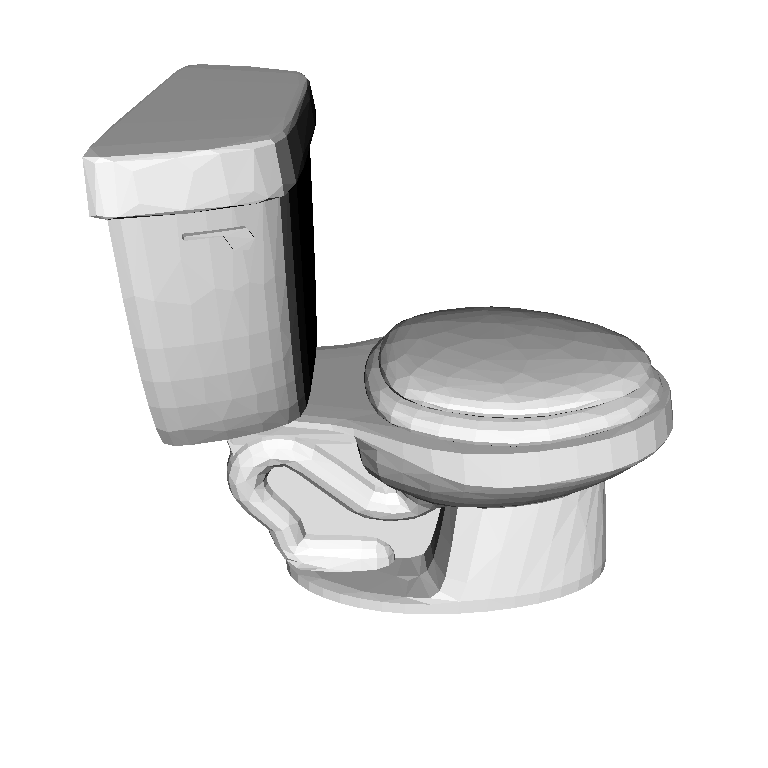
\includegraphics[width=0.15\textwidth]{Figures/ObjRecog/toilet_4}\hfill

	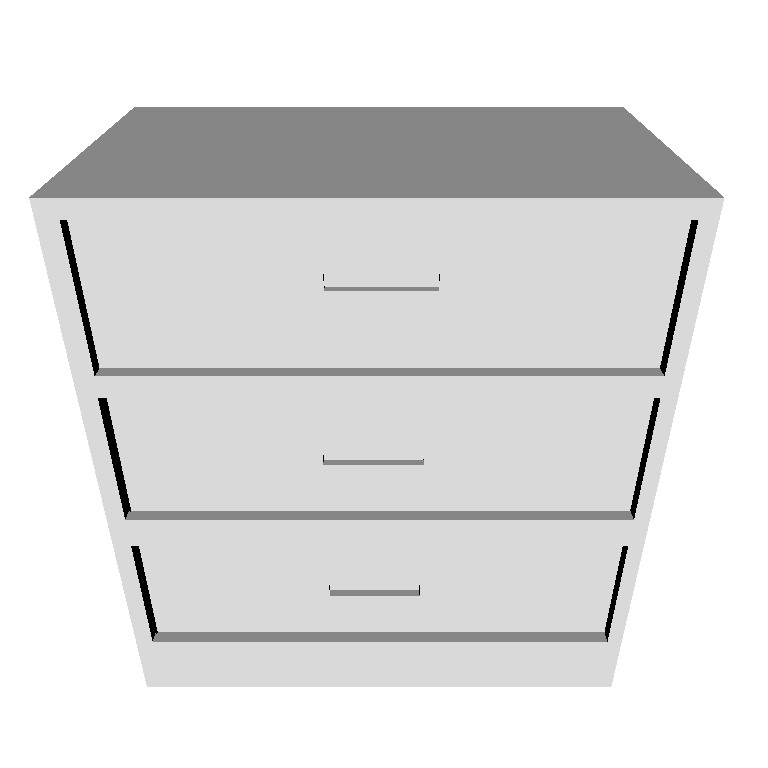
\includegraphics[width=0.15\textwidth]{Figures/ObjRecog/dresser_0}\hfill
	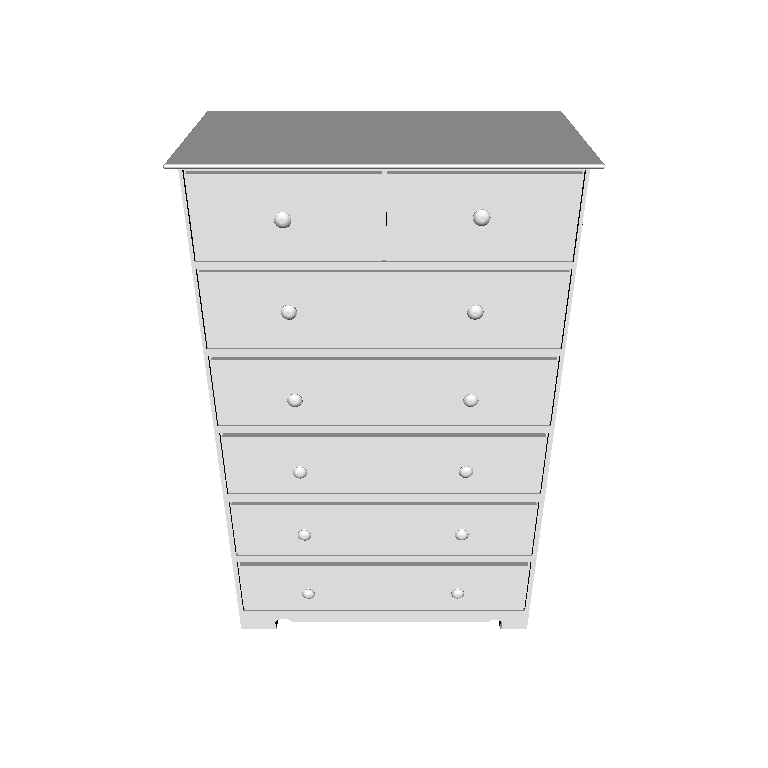
\includegraphics[width=0.15\textwidth]{Figures/ObjRecog/dresser_1}\hfill
	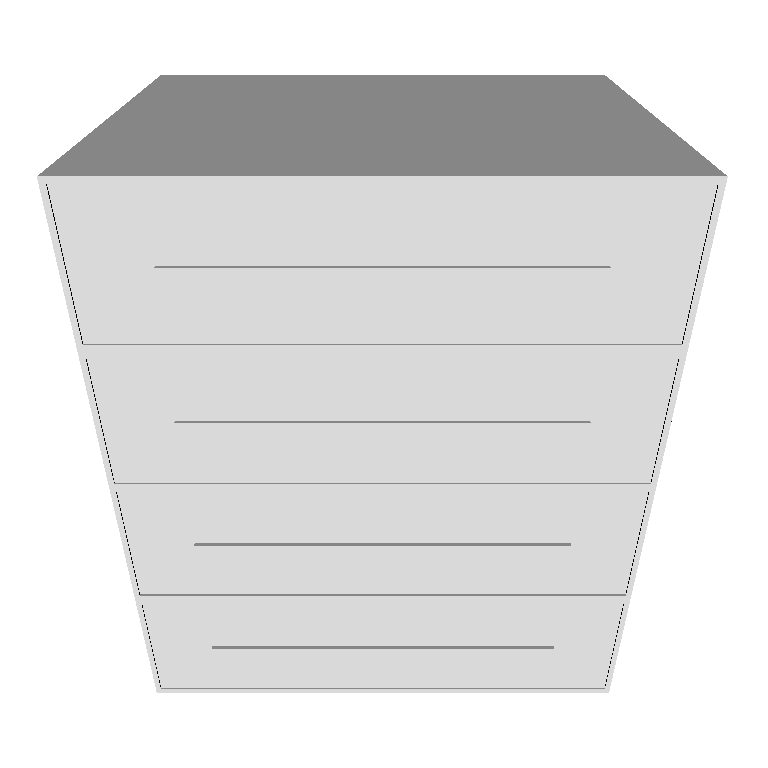
\includegraphics[width=0.15\textwidth]{Figures/ObjRecog/dresser_2}\hfill
	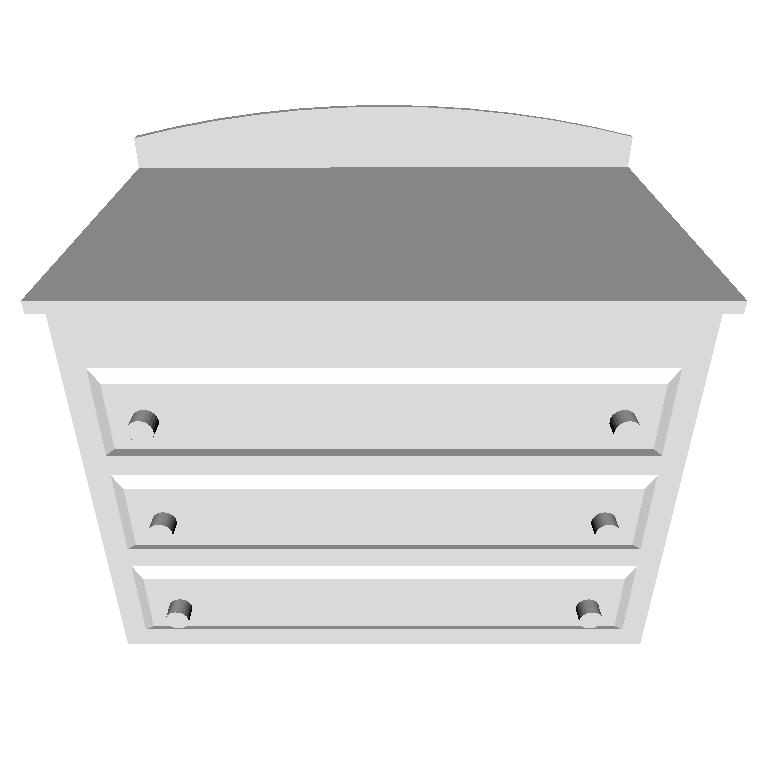
\includegraphics[width=0.15\textwidth]{Figures/ObjRecog/dresser_3}\hfill
	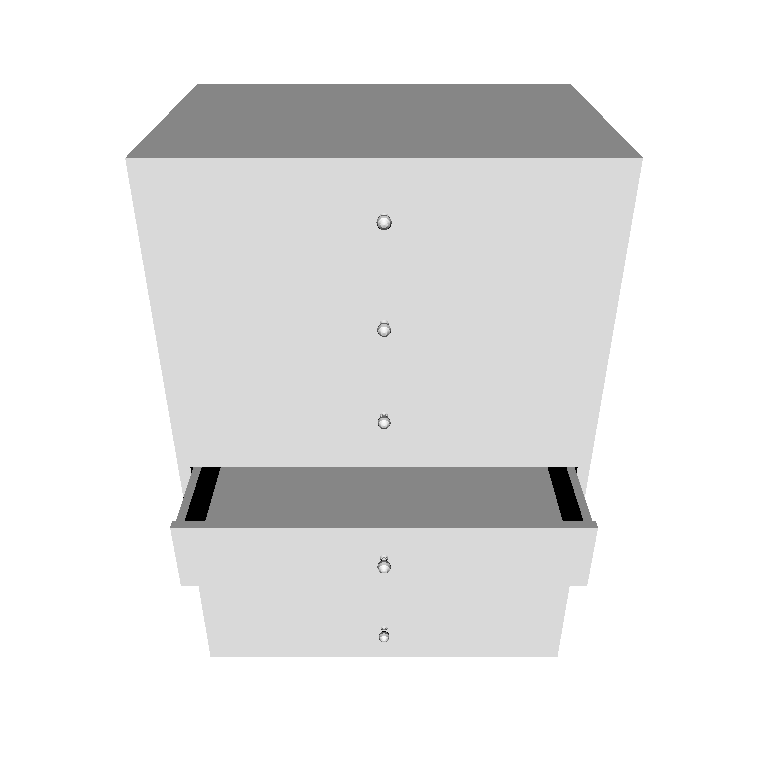
\includegraphics[width=0.15\textwidth]{Figures/ObjRecog/dresser_4}\hfill
	
	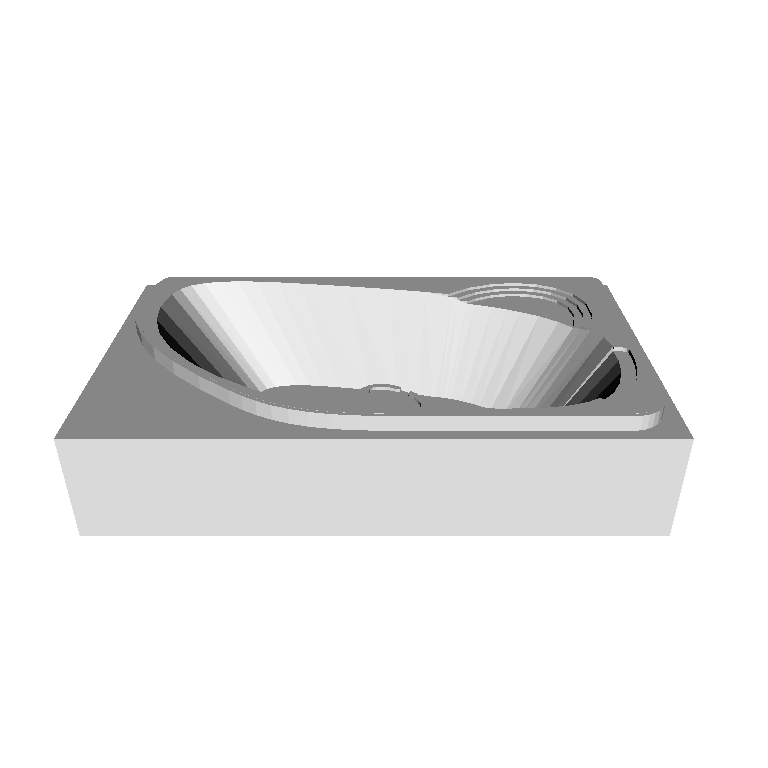
\includegraphics[width=0.15\textwidth]{Figures/ObjRecog/bathtub_0}\hfill
	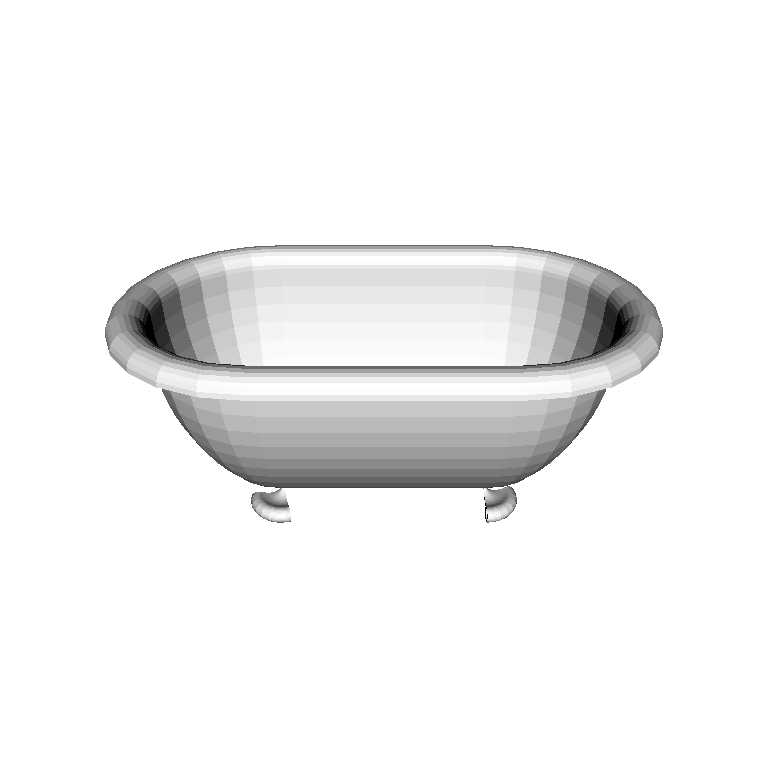
\includegraphics[width=0.15\textwidth]{Figures/ObjRecog/bathtub_1}\hfill
	\includegraphics[width=0.15\textwidth]{Figures/ObjRecog/bathtub_2}\hfill
	\includegraphics[width=0.15\textwidth]{Figures/ObjRecog/bathtub_3}\hfill
	\includegraphics[width=0.15\textwidth]{Figures/ObjRecog/bathtub_4}\hfill

	\includegraphics[width=0.15\textwidth]{Figures/ObjRecog/sofa_0}\hfill
	\includegraphics[width=0.15\textwidth]{Figures/ObjRecog/sofa_1}\hfill
	\includegraphics[width=0.15\textwidth]{Figures/ObjRecog/sofa_2}\hfill
	\includegraphics[width=0.15\textwidth]{Figures/ObjRecog/sofa_3}\hfill
	\includegraphics[width=0.15\textwidth]{Figures/ObjRecog/sofa_4}\hfill

	\includegraphics[width=0.15\textwidth]{Figures/ObjRecog/monitor_0}\hfill
	\includegraphics[width=0.15\textwidth]{Figures/ObjRecog/monitor_1}\hfill
	\includegraphics[width=0.15\textwidth]{Figures/ObjRecog/monitor_2}\hfill
	\includegraphics[width=0.15\textwidth]{Figures/ObjRecog/monitor_3}\hfill
	\includegraphics[width=0.15\textwidth]{Figures/ObjRecog/monitor_4}\hfill

	\includegraphics[width=0.15\textwidth]{Figures/ObjRecog/chair_0}\hfill
	\includegraphics[width=0.15\textwidth]{Figures/ObjRecog/chair_1}\hfill
	\includegraphics[width=0.15\textwidth]{Figures/ObjRecog/chair_2}\hfill
	\includegraphics[width=0.15\textwidth]{Figures/ObjRecog/chair_3}\hfill
	\includegraphics[width=0.15\textwidth]{Figures/ObjRecog/chair_4}\hfill
	\caption{ModelNet10 samples.}
	\label{fig:objrecog:modelnet_models}
\end{figure}

\clearpage

\begin{figure}[!h]
    \centering
    \begin{tikzpicture}
	\begin{axis}[
		ybar,
		width=\linewidth,
		height=20 em,
		ylabel=Models,
		xlabel=Class,
		ymajorgrids=true,
		xtick pos=left,
		enlarge x limits=0.05,
		legend style={at={(0.97,0.97)},anchor=north east},
		xticklabel style = {font=\tiny,},
		ybar=1pt,
		bar width=1.25 pt,
		xmin=1,
		xmax=40,
		ymin=0,
		ymax=1000,
		ytick={0,100,...,1000},
		xtick=data,
		axis on top=false,
		y tick style={uablue50},
		x tick style={uablue50},
		major grid style={very thin, uagray10},
		minor grid style={very thin, uagray10},
		axis line style={uablue50},
		]
			\addplot [color=uablue, fill=uablue] coordinates {(1, 200) (2, 392) (3, 200) (4, 515) (5, 344) (6, 200) (7, 106) (8, 680) (9, 465) (10, 889) (11, 0) (12, 0) (13, 0) (14, 0) (15, 0) (16, 0) (17, 0) (18, 0) (19, 0) (20, 0) (21, 0) (22, 0) (23, 0) (24, 0) (25, 0) (26, 0) (27, 0) (28, 0) (29, 0) (30, 0) (31, 0) (32, 0) (33, 0) (34, 0) (35, 0) (36, 0) (37, 0) (38, 0) (39, 0) (40, 0)};
			\addplot [color=uabranchblue, fill=uabranchblue] coordinates {(1, 86) (2, 100) (3, 86) (4, 100) (5, 100) (6, 86) (7, 50) (8, 100) (9, 100) (10, 100) (11, 0) (12, 0) (13, 0) (14, 0) (15, 0) (16, 0) (17, 0) (18, 0) (19, 0) (20, 0) (21, 0) (22, 0) (23, 0) (24, 0) (25, 0) (26, 0) (27, 0) (28, 0) (29, 0) (30, 0) (31, 0) (32, 0) (33, 0) (34, 0) (35, 0) (36, 0) (37, 0) (38, 0) (39, 0) (40, 0)};
			\addplot [color=uablue30, fill=uablue30] coordinates {(1, 200) (2, 392) (3, 200) (4, 515) (5, 344) (6, 200) (7, 106) (8, 680) (9, 465) (10, 889) (11, 626) (12, 173) (13, 572) (14, 335) (15, 64) (16, 197) (17, 197) (18, 79) (19, 138) (20, 109) (21, 149) (22, 171) (23, 155) (24, 145) (25, 124) (26, 149) (27, 284) (28, 88) (29, 231) (30, 240) (31, 104) (32, 115) (33, 128) (34, 124) (35, 90) (36, 163) (37, 267) (38, 475) (39, 87) (40, 103)};
			\addplot [color=ualightblue, fill=ualightblue] coordinates {(1, 86) (2, 100) (3, 86) (4, 100) (5, 100) (6, 86) (7, 50) (8, 100) (9, 100) (10, 100) (11, 100) (12, 20) (13, 100) (14, 100) (15, 20) (16, 100) (17, 20) (18, 20) (19, 20) (20, 20) (21, 20) (22, 100) (23, 100) (24, 20) (25, 20) (26, 20) (27, 100) (28, 20) (29, 100) (30, 100) (31, 20) (32, 100) (33, 20) (34, 20) (35, 20) (36, 20) (37, 100) (38, 100) (39, 20) (40, 20)};
	\legend{ModelNet-10 training, ModelNet-10 test, ModelNet-40 training, ModelNet-40 test} 
	\end{axis} 
\end{tikzpicture}

    \caption{Model distribution per object class or category for both ModelNet-10 and ModelNet-40 training and test splits.}
    \label{fig:objrecog:modelnet_distribution}
\end{figure}

\begin{figure}[!htb]
	\centering
	\resizebox{\textwidth}{!}{
		\begin{tikzpicture}
%\node[] (cad_model) at (0, 0) {\includegraphics[width=4.5em]{Figures/ObjRecog/adapter/cad_model}};
\node[] (cad_model) at (0, 0) {\includegraphics[width=8em]{Figures/ObjRecog/adapter/sphere_cad}};
\node[above = 0 em of cad_model]  (l1) {CAD Model};
\node[right = 2 em of cad_model] (depth_1) {\includegraphics[width=5em]{Figures/ObjRecog/adapter/depth_1_4}};
\node[above = -1 em of depth_1] (depth_2) {\includegraphics[width=5em]{Figures/ObjRecog/adapter/depth_2_13}};
\node[below = -1 em of depth_1] (depth_3) {\includegraphics[width=5em]{Figures/ObjRecog/adapter/depth_4_31}};
\node[above = 0 em of depth_2]  (l2) {Rendered views};
\node[right = 2 em of depth_1] (cloud_1) {\includegraphics[width=5em]{Figures/ObjRecog/adapter/cloud_1}};
\node[right = 2 em of depth_2] (cloud_2) {\includegraphics[width=5em]{Figures/ObjRecog/adapter/cloud_2}};
\node[right = 2 em of depth_3] (cloud_3) {\includegraphics[width=5em]{Figures/ObjRecog/adapter/cloud_4}};
\node[above = 0 em of cloud_2]  (l3) {Cloud views};
\node[right = 2 em of cloud_1] (cloud) {\includegraphics[width=4.5em]{Figures/ObjRecog/adapter/cloud}};
\node[above = 1 em of cloud]  (l4) {Merged cloud};
%
\draw[uagray80, -latex](cad_model) -- (depth_1);
\draw[uagray80,-latex](cad_model) -- (depth_2);
\draw[uagray80,-latex](cad_model) -- (depth_3);
%
\draw[uagray80, -latex](depth_1) -- (cloud_1);
\draw[uagray80, -latex](depth_2) -- (cloud_2);
\draw[uagray80, -latex](depth_3) -- (cloud_3);
%
\draw[uagray80, -latex](cloud_1) -- (cloud);
\draw[uagray80, -latex](cloud_2) -- (cloud);
\draw[uagray80, -latex](cloud_3) -- (cloud);
\end{tikzpicture}

	}
	\caption{From \acs{CAD} models to point clouds. The object is placed in the center of a tessellated sphere, views are rendered placing a virtual camera in each vertex of the icosahedron, the $z$-buffer data of those views is used to generate point clouds, and the point clouds are transformed and merged at last.}
	\label{fig:objrecog:adapter}
\end{figure}

\clearpage

\begin{table}
    \centering
    \begin{tabular}{rccccc}
    &	\multicolumn{2}{c}{\textbf{\emph{ModelNet-10}}} & \multicolumn{2}{c}{\textbf{\emph{ModelNet-40}}}\\
    \textbf{ID} & \textbf{Category}  & \textbf{Training Set} & \textbf{Test set} & \textbf{Training Set} & \textbf{Test set} \\
    \toprule
    1 & Desk      & 200        & 86		& 200  & 86     \\
    2 & Table     & 392        & 100    & 392  & 100	\\
    3 & Nighstand & 200        & 86     & 200  & 86		\\
    4 & Bed       & 515        & 100    & 515  & 100	\\
    5 & Toilet    & 344        & 100    & 344  & 100	\\
    6 & Dresser   & 200        & 86     & 200  & 86		\\
    7 & Bathtub   & 106        & 50     & 106  & 50		\\
    8 & Sofa      & 680        & 100    & 680  & 100	\\
    9 & Monitor   & 465        & 100    & 465  & 100 	\\
    10 & Chair     & 889        & 100    & 889  & 100	\\
    11 & Airplane  & -	 & -	 & 626	& 100 \\
    12 & Bench	  & -	 & -	 & 173	& 20 \\
    13 & Bookshelf & -	 & -	 & 572	& 100 \\
    14 & Bottle	  & -	 & -	 & 335	& 100 \\
    15 & Bowl	  & -	 & -	 & 64	& 20 \\
    16 & Car		  & -	 & -	 & 197	& 100 \\
    17 & Cone	  & -	 & -	 & 167	& 20 \\
    18 & Cup		  & -	 & -	 & 79	& 20 \\
    19 & Curtain	  & -	 & -	 & 138	& 20 \\
    20 & Door	  & -	 & -	 & 109	& 20 \\
    21 & Flower Pot & -	 & -	 & 149	& 20 \\
    22 & Glass Box & -	 & -	 & 171	& 100 \\
    23 & Guitar	  & -	 & -	 & 155	& 100 \\
    24 & Keyboard  & -	 & -	 & 145	& 20 \\
    25 & Lamp	  & -	 & -	 & 124	& 20 \\
    26 & Laptop	  & -	 & -	 & 149	& 20 \\
    27 & Mantel	  & -	 & -	 & 284	& 100 \\
    28 & Person	  & -	 & -	 & 88	& 20 \\
    29 & Piano	  & -	 & -	 & 231	& 100 \\
    30 & Plant	  & -	 & -	 & 240	& 100 \\
    31 & Radio	  & -	 & -	 & 104  & 20 \\
    32 & Range Hood & -	 & -	 & 115	& 100 \\
    33 & Sink	  & -	 & -	 & 128	& 20 \\
    34 & Stairs 	 & -	 & -	 & 124	& 20 \\
    35 & Stool 	 & -	 & -	 & 90	& 20 \\
    36 & Tent  	 & -	 & -	 & 163	& 20 \\
    37 & TV Stand  & -	 & -	 & 267	& 100 \\
    38 & Vase	 & -	 & -	 & 475	& 100 \\
    39 & Wardrobe  & -	 & -	 & 87	& 20 \\
    40 & X-Box	 & -	 & -	& 103	& 20 \\
    \bottomrule
    \end{tabular}
    \caption{ModelNet-10 and ModelNet-40 distributions.}
    \label{table:objrecog:modelnet_distribution}
\end{table}

\clearpage

For this purpose, we converted the \ac{OFF} models into \ac{PCD} clouds using a raytracing-based process. The object is placed in the center of a \acs{3D} sphere, which is tessellated to a certain level, and a virtual camera pointing to the center of the sphere is placed in each vertex of that truncated icosahedron. Then those partial views are rendered and their $z$-buffer data, which contains the depth information, is used to generate point clouds from each \acs{PoV}. In the end, those views are translated and rotated, depending on their \ac{PoV}, and merged into a cloud for the full object.

Figure \ref{fig:objrecog:adapter} shows a diagram of the aforementioned process. For the conversion, we used the first tessellation level of the sphere, which generates $42$ vertices or \acp{PoV}. A resolution of $256\times256$ pixels was used for rendering the views. A voxel grid filter with a leaf size of $0.7\times0.7\times0.7$ units is applied to the merged cloud to equalize the point density, which is higher in certain zones due to view overlapping.


\section{PointNet}
\label{cha:objrecog:sec:pointnet}

In this first iteration of our efforts towards an object class recognition solution, we propose a system that takes a point cloud of an object as input and predicts its class label by leveraging two novel components: (1) a point density volumetric grid to estimate spatial occupancy inside each voxel, and (2) a \ac{3D}-\ac{CNN} which is trained to predict object classes from those grids. The occupancy grid -- inspired by VoxNet's \cite{Maturana2015} occupancy models that rely on probabilistic estimates -- provides a compact representation of the object's \ac{3D} information originally present in the point cloud that can be fed to the \ac{CNN} architecture, which in turn computes a label for that sample, i.e., predicts the class of the object. 

The components of this approach, namely \emph{PointNet}, will be described throughout this section, which is organized as follows. Firstly, the proposed data representation is introduced in Section \ref{cha:objrecog:sec:pointnet:subsec:data}. Secondly, the network itself is presented in Section \ref{cha:objrecog:sec:pointnet:subsec:network}. Next, we carry out a set of experiments to validate the system in Section \ref{cha:objrecog:sec:pointnet:subsec:experiments}. At last, in Section \ref{cha:objrecog:sec:pointnet:subsec:conclusion}, we draw conclusions about this work and set the stage for the next iteration.

\subsection{Data Representation}
\label{cha:objrecog:sec:pointnet:subsec:data}

As we mentioned before, our proposed architecture takes a point cloud of an object as input to recognize it. However, point clouds are unstructured representations that cannot be easily handled by common \ac{CNN} architectures due to the lack of a matrix-like organization. The most straightforward way to apply formal convolutions to that unstructured space is to impose a certain organization into it. Occupancy grids expose a compact representation of the volumetric space: they stand between meshes or clouds, which offer rich but unstructured information, and voxelized representations, with packed but poor information. At that midpoint, occupancy grids provide important shape cues to perform learning while enabling an efficient processing of that information.

As we previously reviewed in Section \ref{cha:objrecog:sec:relatedworks}, certain 3D deep learning architectures make use of occupancy grids as a representation for the input data. For instance, 3D ShapeNets \cite{Wu2015} is a \ac{CDBN} which represents a 3D shape as a $30 \times 30 \times 30$ binary tensor in which a one indicates that a voxel intersects the mesh surface, and a zero represents empty space. VoxNet \cite{Maturana2015} introduces three different occupancy grids that employ 3D ray tracing to compute the number of beams hitting or passing each voxel and then use that information to compute the value of each voxel depending on the chosen model: a binary occupancy grid using probabilistic estimates, a density grid in which each voxel holds a value corresponding to the probability that it will block a sensor beam, and a hit grid that only considers hits thus ignoring empty or unknown space. The binary and density grids proposed by Maturana \emph{et al.} \cite{Maturana2015} differentiate unknown and empty space, whilst the hit grid and the binary tensor do not. VoxNet's occupancy grid outperforms 3D ShapeNets in terms of accuracy in the ModelNet challenge for the 3D-centric approaches described above. However, ray tracing grids considerably harmed runtime so that other approaches must be considered for a real-time implementation.

\begin{figure}[!t]
  \centering
  \begin{subfigure}{0.3\linewidth}
    \centering
    \includegraphics[width=0.9\linewidth]{Figures/ObjRecog/detergent_mesh.png}
    \caption{Mesh}
    \label{fig:objrecog:meshcloudgrid:mesh}
  \end{subfigure}
  \begin{subfigure}{0.3\linewidth}
    \centering
    \includegraphics[width=0.9\linewidth]{Figures/ObjRecog/detergent_cloud.png}
    \caption{Cloud}
    \label{fig:objrecog:meshcloudgrid:cloud}
  \end{subfigure}
  \begin{subfigure}{0.3\linewidth}
    \centering
    \includegraphics[width=0.8\linewidth]{Figures/ObjRecog/detergent_grid.png}
    \caption{Grid}
    \label{fig:objrecog:meshcloudgrid:grid}
  \end{subfigure}
  \caption{Various 3D representations for an object. A mesh (\subref{fig:objrecog:meshcloudgrid:mesh}) is transformed into a point cloud (\subref{fig:objrecog:meshcloudgrid:cloud}), and that cloud is processed to obtain a voxelized occupancy grid (\subref{fig:objrecog:meshcloudgrid:grid}). The occupancy grid shown in this figure is a cube of $30\times 30 \times 30$ voxels. Each voxel of that cube holds the point density inside its volume. In this case, dark voxels indicate high density whilst bright ones are low density.}
  \label{fig:objrecog:meshcloudgrid}
\end{figure}

With PointNet, we propose an occupancy grid inspired by the aforementioned successes but aiming to maintain a reasonable accuracy while enabling a real-time implementation. In our volumetric representation, each point of a cloud is mapped to a voxel of a fixed-size occupancy grid. Before performing that mapping, the object cloud is scaled to fit the grid. Each voxel will hold a value representing the number of points mapped to itself. At last, the values held by each cell are normalized. Figure \ref{fig:objrecog:meshcloudgrid} shows the derivation of the proposed occupancy grid representation from other typical tridimensional representations of a sample object.

\subsection{Network Architecture}
\label{cha:objrecog:sec:pointnet:subsec:network}

As we have previously stated, \acp{CNN} have proven to be very useful for recognizing and classifying objects in \ac{2D} images. A convolutional layer can recognize basic patterns such as corners or planes and if we stack several of them they can learn a topology of hierarchical filters. Furthermore, the composition of several of these regions can define a feature of a more complex object. By doing that, a combination of various filters is able to recognize a full object. We apply this approach used in \ac{2D} images to \ac{3D} recognition. Our PointNet architecture features two convolutional layers $(m, n, d)$, which convolve the data in batches of $n\times n\times n$ voxels with $m$ learnable filters and a stride of $d$; pooling layers $(n, d)$, which perform max-pooling with a filter size of $n$ and a stride of $d$; Inner Product layers $(n)$, that are fully connected layers with $n$ neurons; and \ac{ReLU} layers after each convolution and the first Inner Product one. The deep architecture featured by \emph{PointNet} is represented in Figure \ref{fig:objrecog:pointnetarch}.

\begin{figure}[!b]
	\resizebox{\linewidth}{!}{
	\begin{tikzpicture}
			\tikzset{
            block/.style={minimum width=12em, minimum height=3 em, draw=black, very thick},}
            \node [block] (pcdl) at (0,0) {\textbf{PC Data Layer} (300, 5)};
            \node [block, right = 2 em of pcdl.east] (conv) {\textbf{Convolution}(48, 3, 1)};
            \node [block, right = 2 em of conv.east] (pool) {\textbf{Pooling}(3, 2)};
            \node [block, right = 2 em of pool.east] (conv2) {\textbf{Convolution}(160, 3, 2)};
            \node [block, below = 2 em of conv2.south] (pool2) {\textbf{Pooling}(2, 2)};
            \node [block, left = 2 em of pool2.west] (inner) {\textbf{Inner Layer}(1000)};
            \node [block, left = 2 em of inner.west] (inner2) {\textbf{Inner Layer}(10)};
            \node [block, left = 2 em of inner2.west] (softmax) {\textbf{Softmax with Loss}};
            \draw[-latex, very thick] (pcdl.east) -- (conv.west);
            \draw[-latex, very thick] (conv.east) -- (pool.west);
            \draw[-latex, very thick] (pool.east) -- (conv2.west);
            \draw[-latex, very thick] (conv2.south) -- (pool2.north);
            \draw[-latex, very thick] (pool2.west) -- (inner.east);
            \draw[-latex, very thick] (inner.west) -- (inner2.east);
            \draw[-latex, very thick] (inner2.west) -- (softmax.east);
    \end{tikzpicture}}
    \caption{\emph{PointNet} \acl{CNN} architecture.}
    \label{fig:objrecog:pointnetarch}
\end{figure}

\subsection{Experiments}
\label{cha:objrecog:sec:pointnet:subsec:experiments}

In order to evaluate the performance of our proposed representation and network, we carried out a set of experiments using the ModelNet-10 dataset. Those experiments aim to prove that the network is able to achieve reasonable accuracy while still being able to execute in real time. Furthermore, we also study ways to increase our performance by analyzing our data, e.g., the balance between classes in the dataset and the possible sources of confusion that make learning harder. To that end, we first describe our data generation process as well as the experimentation methodology (implementation details and test setup); then we show our experiments together with a discussion for each one of them to keep on building and experimenting in an incremental way.

\begin{figure}[!htb]
  \centering
  \begin{subfigure}{\linewidth}
    \includegraphics[width=0.24\linewidth]{Figures/ObjRecog/toilet_0_view}
    \includegraphics[width=0.24\linewidth]{Figures/ObjRecog/toilet_1_view}
    \includegraphics[width=0.24\linewidth]{Figures/ObjRecog/toilet_2_view}
    \includegraphics[width=0.24\linewidth]{Figures/ObjRecog/toilet_3_view}
    \caption{Rendered views.}
    \label{fig:objrecog:dataproc:renders}
  \end{subfigure}
  \begin{subfigure}{0.32\linewidth}
    \includegraphics[width=0.9\linewidth]{Figures/ObjRecog/toilet_off.png}
    \caption{Mesh.}
    \label{fig:objrecog:dataproc:mesh}
  \end{subfigure}
  \begin{subfigure}{0.32\linewidth}
    \includegraphics[width=0.9\linewidth]{Figures/ObjRecog/toilet_cloud.png}
    \caption{Cloud.}
    \label{fig:objrecog:dataproc:cloud}
  \end{subfigure}
  \begin{subfigure}{0.32\linewidth}
    \includegraphics[width=0.9\linewidth]{Figures/ObjRecog/toilet_cloud_downsampled.png}
    \caption{Downsampled.}
    \label{fig:objrecog:dataproc:downsampled}
  \end{subfigure}
  \caption{Dataset model processing example to generate the point clouds for PointNet. Some rendered views of a toilet model are shown in (\subref{fig:objrecog:dataproc:renders}). The original \ac{OFF} mesh is shown in (\subref{fig:objrecog:dataproc:mesh}). The generated point cloud after merging all points of view is shown in (\subref{fig:objrecog:dataproc:cloud}), and (\subref{fig:objrecog:dataproc:downsampled}) shows the downsampled cloud using a voxel grid filter with a leaf size of $0.7 \times 0.7 \times 0.7$.}
  \label{fig:objrecog:pointnetarchdata}
\end{figure}

\subsubsection{Data Generation}

We generated point clouds to feed PointNet following the procedure described in Section \ref{cha:objrecog:sec:datasets}. Figure \ref{fig:objrecog:pointnetarchdata} illustrates the result of the aforementioned process. After that, the resulting point clouds are used to train, randomizing the order of the models, and test the system taking into account the corresponding splits provided by ModelNet-10.

\subsubsection{Implementation and Setup}

This architecture was implemented using the \ac{PCL} \cite{Rusu2011}\cite{Aldoma2012} – which provides state-of-the-art algorithm implementations for 3D point cloud processing – and Caffe \cite{Jia2014}, a deep learning framework developed and maintained by the \ac{BVLC} and an active community of contributors on GitHub. This BSD-licensed C++ library enables researchers to design, train, and deploy \ac{CNN} architectures efficiently, mainly thanks to its drop-in integration of NVIDIA cuDNN \cite{Chetlur2014} to take advantage of \ac{GPU} acceleration.

All the timings and results were obtained by performing the experiments in the following test setup: Intel Core i5-3570 with 8 GB of 1600 MHz DD3 RAM on an ASUS P8H77-M PRO motherboard (Intel H77 chipset). Additionally, the system includes an NVIDIA Tesla K20 GPU, and a Seagate Barracuda 7200.14 secondary storage. Caffe RC2 was run over ElementaryOS Freya 0.3.1, an Ubuntu-based Linux distribution. It was compiled using CMake 2.8.7, g++ 4.8.2, CUDA 7.0, and cuDNN v3.

\subsubsection{Results and Discussion}
\label{cha:objrecog:sec:pointnet:subsec:discussion}

The first experiment just consisted of training the vanilla network to establish a baseline upon which we could build future improments. To do so, we trained \emph{PointNet} using \ac{SGD} with a learning rate of $1e^{-4}$ and a momentum of $9e^{-1}$ during $200$ iterations with early stopping. This first experimental iteration achieved and accuracy rate of $77.6$\% in the test set. As shown in Table \ref{table:objrecog:pointnet:confusion}, the confusion matrix reveals the stability of the system, mainly confusing items that look alike such as desk and table. Because of the nature of \acp{CNN}, which heavily rely on detecting combinations of features, these kind of errors are common. As we can observe in Figure \ref{fig:objrecog:tabledesk}, the visual features that define a desk and a table are almost the same, making it hard to distinguish between both classes. Figure \ref{fig:objrecog:tabledesk_activations} shows the neuron activations for the output layer of the architecture, proving that \emph{Desk} and \emph{Table} are consistently confused in the test set. In light of those experiments it is conceivable to think that a deeper network would provide better results by being able to model the subtleties of such small differences.

\begin{table}[!htb]
\centering
\pgfplotstabletypeset[color cells]{
    Desk, Table, Nstand, Bed, Toilet, Dresser, Batht, Sofa, Mntr, Chair	
    52, 9, 1, 4, 0, 5, 1, 5, 0, 9
    25, 69, 0, 1, 0, 0, 0, 0, 1, 4
    1, 2, 60, 1, 4, 8, 0, 0, 2, 8
    4, 0, 0, 80, 0, 0, 3, 11, 1, 1
    1, 0, 3, 1, 84, 0, 1, 3, 2, 5
    3, 0, 14, 0, 0, 61, 0, 1, 6, 1
    0, 1, 0, 3, 0, 0, 34, 8, 3, 1
    1, 0, 1, 4, 1, 2, 0, 88, 1, 2
    1, 1, 1, 1, 0, 5, 1, 1, 87, 2
    1, 2, 1, 2, 1, 1, 0, 1, 1, 90
}
\caption{Confusion matrix for the first set of experiments making use of the vanilla \emph{PointNet} architecture. Notice the high amount of confusion in the Desk-Table pair.}\label{table:objrecog:pointnet:confusion}
\end{table}

\begin{figure}[!htb]
    \centering
    \begin{subfigure}{0.49\linewidth}
        \includegraphics[width=\linewidth]{Figures/ObjRecog/table}
        \caption{}
        \label{subfig:objrecog:tabledesk:table}
    \end{subfigure}
    \begin{subfigure}{0.49\linewidth}
        \includegraphics[width=\linewidth]{Figures/ObjRecog/desk}
        \caption{}
        \label{subfig:objrecog:tabledesk:desk}
    \end{subfigure}
    \caption{Similarity between two objects of different classes: Table and Desk. The point cloud shown in (\subref{subfig:objrecog:tabledesk:table}) represents an object of the Table class, whilst the point cloud in (\subref{subfig:objrecog:tabledesk:desk}) represents an object whose class is Desk but it is misclassified as a Table due to their resemblance.}
    \label{fig:objrecog:tabledesk}
\end{figure}

\begin{figure}[!htb]
    \centering
    \begin{subfigure}{0.49\linewidth}
        \includegraphics[width=\linewidth]{Figures/ObjRecog/table_matrix}
        \caption{}
        \label{subfig:objrecog:tabledesk_activations:table}
    \end{subfigure}
    \begin{subfigure}{0.49\linewidth}
        \includegraphics[width=\linewidth]{Figures/ObjRecog/desk_matrix}
        \caption{}
        \label{subfig:objrecog:tabledesk_activations:desk}
    \end{subfigure}
    \caption{Neuron activations for the output layer of the architecture when classifying all the test samples for both \emph{Desk}(\subref{subfig:objrecog:tabledesk_activations:desk}) and \emph{Table}(\subref{subfig:objrecog:tabledesk_activations:table}) classes. Each row represents an activation vector for a specific sample, so each column is a position of the vector: the activation to that particular class. The first column corresponds to the \emph{Desk} class, while the second one is the \emph{Table}. The activation shows the clear confusion between \emph{Desk} and \emph{Table}. Although the latter one is much less confused with other classes, many \emph{Tables} are misclassified as \emph{Desks} thus lowering the accuracy for this class.}
    \label{fig:objrecog:tabledesk_activations}
\end{figure}

For the deeper network experiment we added several layers to the vanilla \emph{PointNet} architecture. One more convolutional layer was added since these layers are coupled to the detection of the features of the objects, so the more layers induce a more complex or expressive model. Another fully connected or inner product layer was also added. Since these layers make the classification possible, making that classifier deeper would theoretically make us able to provide better classification results. Despite all those theoretical improvements, one must also consider that we are also introducing more parameters in the network thus making it harder to train and prone to overfitting the train data.

This architecture was trained during $1.000$ iterations to account for that increase in training difficulty. The best result was provided at $800$ iterations with an accuracy of $76.7$\% in the test set. Those models that kept on training dropped performance to $75.9$\% due to overfitting. Surprisingly, increasing the depth of the network did not help rising test accuracy. Because of that, we decided to investigate our data to check if any factor was hindering the training process.

Training using an unbalanced dataset tends to harm those classes with the least number of examples and to benefit those with the most \cite{Dalyak2014}. Having this in mind, and knowing that ModelNet-10 is highly unbalanced as shown in Table \ref{table:objrecog:modelnet_distribution}, the dataset was balanced by limiting the number of examples of each class to $400$ samples using random undersampling. This does not fully solve the problem but makes the difference between classes with the least number of examples and those with the most least acute. The network was trained and tested again with this more balanced dataset and the best performer achieved a test accuracy of $72.9$\%. Again, this experiment did not result into any gain but rather made our network perform worse. The fact is that balancing the training set makes the accuracy of the classes with less examples higher, but it harms the success rate on classes with more instances as seen in Figure \ref{fig:objrecog:balunbal}. The improvement on those less represented classes is not enough to make up for the impact on the most represented ones.

\begin{figure}[!htb]
    \centering
    \begin{tikzpicture}
        \begin{axis}[
            height=6cm,
            width=0.8\linewidth,
            ylabel={Accuracy $[\% /100]$},
            xlabel={Class $[ID]$},
            ymajorgrids=true,
            legend pos=south east,
            xtick pos=left,
            enlarge x limits=0.15,
            ybar=2pt,
            bar width=5 pt,
            xmin=1,
            xmax=10,
            ymin=0,
            ymax=1.0,
            ytick={0.0,0.1,...,1.1},
            xtick=data,
            axis on top=false,]
            \addplot [color=uagray80, fill=uablue50] coordinates {(1, 0.9) (2, 0.72) (3, 0.8) (4, 0.9) (5, 0.69) (6, 0.57) (7, 0.57) (8, 0.56) (9, 0.59) (10, 0.64)};
            \addplot [color=uagray80, fill=uablue10] coordinates {(1, 0.68) (2, 0.71) (3, 0.69) (4, 0.75) (5, 0.74) (6, 0.65) (7, 0.62) (8, 0.8) (9, 0.85) (10, 0.72)};
            \legend{Unbalanced, Balanced}
        \end{axis}
    \end{tikzpicture}
    \caption{Comparison of accuracy per class using an unbalanced dataset and a balanced one with a maximum of $400$ models per class via random undersampling. Accuracy is harmed in the classes in which models are removed but gained otherwise.}
    \label{fig:objrecog:balunbal}
\end{figure}

After analyzing the results, it can be stated that neither a deeper network nor balancing the dataset increase accuracy. In fact, the experiments of the original architecture with the unbalanced ModelNet-10 exhibited better performance with a $77.6$\% success rate. In addition, \emph{PointNet} takes an average time of $24.6$ milliseconds to classify an example (in comparison with \emph{VoxNet}, which can take up to half a second for its raytracing-based implementation). These results prove the system as a fast and accurate \ac{3D} object class recognition tool.

\subsection{Conclusion}
\label{cha:objrecog:sec:pointnet:subsec:conclusion}

\emph{PointNet} is our first approach towards devising an efficient and accurate \ac{CNN} for \ac{3D} object class recognition. It was inspired by other contemporary works such \emph{VoxNet} and \ac{3D} \emph{ShapeNets}, in the sense that it also handles tridimensional data for object recognition. Its contributions lies in the fact that the architecture itself and the representation too were simplified and the whole pipeline was implemented in Caffe thus providing a faster method than the state of art ones yet obtaining a high accuracy rate in the ModelNet-10 dataset.

\section{Noise and Occlusion}
\label{cha:objrecog:sec:study}

Although \emph{PointNet} was a step forward at the time it was released, there were still a set of open questions regarding its effectiveness. Such questions are strongly related to common problems that arise when recognizing objects in real-world scenes: how sensitive is the network to the noise introduced by the sensor? And most importantly, how robust is the network against clutter and occlusions? In this second iteration of our object recognition system we aim to throw some light into such unknowns. To that end, we carry out a study in which we test various data representations and an improved network iterated over the previously introduced \emph{PointNet} network.

This section is organized as follows. First off, we introduce our proposals for robust data representations in Section \ref{cha:objrecog:sec:study:subsec:representation}. In the second place, we discuss the improved network architecture in Section \ref{cha:objrecog:sec:study:subsec:architecture}. After that, the main body of this iteration is presented in Section \ref{cha:objrecog:sec:study:subsec:experiments}: an extensive experimentation to determine the effect of noise and occlusion. In the end, in Section \ref{cha:objrecog:sec:study:subsec:conclusion} we discuss the insights gained thanks to the experimentation and we also set the scene for the last iteration of the object recognition system.

\subsection{Data Representation}
\label{cha:objrecog:sec:study:subsec:representation}

As we already stated previously, a volumetric representation to be fed to a \acs{CNN} must encode the \acs{3D} shape of an object as a \acs{3D} tensor of binary or real values. This is due to the fact that raw \acs{3D} data is sparse, i.e., a \acs{3D} shape is only defined on its surface, and \acp{CNN} are not engineered for this kind of data. However simple this statement might seem, there are many nuances and subtleties in the way such tensors are created and how their values are computed. Those detials may have an important impact on performance in unexpected ways.

In this regard, our proposal for the study is twofold. First, we implemented two different ways of generating the structure of the tensor -- position, grid size, and leaf size -- using a fixed grid and an adaptive one. Second, we developed two possible occupancy measures for the volumetric elements of the tensor.

\newpage

\subsubsection{Tensor Generation}
\label{cha:objrecog:sec:study:subsec:representation:subsubsec:tensor}

Providing that the input to our network consists of point clouds, we need to generate a discretized representation of the unbounded \acs{3D} data to feed the network. Each cloud will be represented as a \acs{3D} tensor so we need to spawn a grid to subdivide the space occupied by the point clouds. Two types are proposed: one with fixed leaf and grid sizes, and another one which will adapt those sizes to fit the data.

\paragraph{Fixed}

This kind of grid sets its origin at the minimum $x$, $y$, and $z$ values of the point cloud. Then the grid is spawned, with fixed and predefined sizes for both grid and voxels. After that, the cloud is scaled up or down to fit the grid. The scale factor is computed with respect to the dimension of maximum difference between the cloud and the grid. The cloud is scaled with that factor in all axes to maintain the original ratios. As a result, a cubic grid is generated as shown in Figure \ref{fig:objrecog:fixed}.

\begin{figure}[!ht]
	\centering
	\hfill
	\begin{subfigure}{0.325\textwidth}
		\centering
		\includegraphics[width=\linewidth]{Figures/ObjRecog/fixed_front}
		\caption{Front}
		\label{subfig:objrecog:fixed:front}
	\end{subfigure}
	\hfill
	\begin{subfigure}{0.325\textwidth}
		\centering
		\includegraphics[width=\linewidth]{Figures/ObjRecog/fixed_side}
		\caption{Side}
		\label{subfig:objrecog:fixed:side}
	\end{subfigure}
	\hfill
	\begin{subfigure}{0.325\textwidth}
		\centering
		\includegraphics[width=\linewidth]{Figures/ObjRecog/fixed_persp}
		\caption{Perspective}
		\label{subfig:objrecog:fixed:persp}
	\end{subfigure}
	\hfill
	\caption{A fixed occupancy grid ($8\times8\times8$ voxels) with $40$ units leaf size and $320$ units grid size in all dimensions. The grid origin is placed at the minimum $x$, $y$, and $z$ values of the point cloud. Front (\subref{subfig:objrecog:fixed:front}), side (\subref{subfig:objrecog:fixed:side}), and perspective (\subref{subfig:objrecog:fixed:persp}) views of the grid over a partial view of a segmented table object are shown.}
	\label{fig:objrecog:fixed}
\end{figure}

\begin{figure}[!htb]
	\centering
	\hfill
	\begin{subfigure}{0.325\textwidth}
		\centering
		\includegraphics[width=\linewidth]{Figures/ObjRecog/adaptive_front}
		\caption{Front}
		\label{subfig:objrecog:adaptive:front}
	\end{subfigure}
	\hfill
	\begin{subfigure}{0.325\textwidth}
		\centering
		\includegraphics[width=\linewidth]{Figures/ObjRecog/adaptive_side}
		\caption{Side}
		\label{subfig:objrecog:adaptive:side}
	\end{subfigure}
	\hfill
	\begin{subfigure}{0.325\textwidth}
		\centering
		\includegraphics[width=\linewidth]{Figures/ObjRecog/adaptive_persp}
		\caption{Perspective}
		\label{subfig:objrecog:adaptive:persp}
	\end{subfigure}
	\hfill
	\caption{An adaptive occupancy grid ($8\times8\times8$ voxels) with adapted leaf and grid sizes in all dimensions to fit the data. The grid origin is placed at the minimum $x$, $y$, and $z$ values of the point cloud. Front (\subref{subfig:objrecog:adaptive:front}), side (\subref{subfig:objrecog:adaptive:side}), and perspective (\subref{subfig:objrecog:adaptive:persp}) views of the grid over a partial view of a segmented table object are shown. Notice that the point clouds for the three views are exactly the same for this figure and Figure \ref{fig:objrecog:fixed}, but the grids do change. There is a noticeable difference in the	front view. In Figure \ref{fig:objrecog:fixed}, using fixed grids, all voxels are cubic and the point cloud does not fit the grid completely (leftmost column in Figure \ref{subfig:objrecog:fixed:front}), whilst in this figure, with adaptive grids, the grid is fitted to the cloud.}
	\label{fig:objrecog:adaptive}
\end{figure}

\paragraph{Adaptive}

The adaptive grid also sets its origin at the minimum $x$, $y$, and $z$ values of the point cloud. Next, the grid size is adapted to the cloud dimensions. The leaf size is also computed in function of the grid size. Knowing both parameters, the grid is spawned, fitting the point cloud data. As a result, a non-cubic grid is generated. As shown in Figure \ref{fig:objrecog:adaptive}, all voxels have the same size, but they are not necessarily cubic.

It is important to remark that, in both cases (fixed and adaptive), the number of voxels in the grid is fixed. Figures \ref{fig:objrecog:fixed} and \ref{fig:objrecog:adaptive} show examples for both types using $8\times8\times8$ voxels for the sake of a better visualization.

It is also important to notice that each representation serves a purpose. The fixed grid will not always fit the data perfectly so it might end up having sparse zones with no information at all (as seen in Figure \ref{subfig:objrecog:fixed:front} on the first column). However, it can be used right away for sliding box detection. On the contrary, the adaptive grid fits the data to achieve a better representation. Nonetheless, it relies on a proper segmentation of the object to spawn the grid.

\subsubsection{Occupancy Computation}
\label{cha:objrecog:sec:study:subsec:representation:subsubsec:occupancy}

After spawning the grid to generate a discrete space, we need to determine the values for each cell or voxel of the \acs{3D} tensor. In order to do that, we must encode the geometric information of the point cloud into each occupied cell (see Figure \ref{fig:objrecog:grid_occ}). In other words, we have to summarize as a single value, the information of all points which lie inside a certain voxel. One way to do that is using occupancy measures. For that purpose, we propose two different alternatives: binary occupancy, normalized density.

\begin{figure}[!htb]
	\centering
	\hfill
	\begin{subfigure}{0.325\textwidth}
		\centering
		\includegraphics[width=\linewidth]{Figures/ObjRecog/surface_grid_front}
		\caption{Front}
		\label{subfig:objrecog:grid_occ:front}
	\end{subfigure}
	\hfill
	\begin{subfigure}{0.325\textwidth}
		\centering
		\includegraphics[width=\linewidth]{Figures/ObjRecog/surface_grid_side}
		\caption{Side}
		\label{subfig:objrecog:grid_occ:side}
	\end{subfigure}
	\hfill
	\begin{subfigure}{0.325\textwidth}
		\centering
		\includegraphics[width=\linewidth]{Figures/ObjRecog/surface_grid_persp}
		\caption{Perspective}
		\label{subfig:objrecog:grid_occ:persp}
	\end{subfigure}
	\hfill
	\caption{Occupied voxels in an adaptive $8\times8\times8$ grid generated over a partial view point cloud. Those voxels with points inside are shown in a wireframe representation. Empty voxels are omitted. Occupied voxels must be filled with values which represent the contained shape.}
	\label{fig:objrecog:grid_occ}
\end{figure}

\paragraph{Binary}

The binary tensor is the simplest representation that can be conceived to encode the shape. Voxels will hold binary values, they will be considered occupied if at least a point lies inside, and empty otherwise. Figure \ref{fig:objrecog:binary_occ} shows an example of this tensor.

\begin{figure}[!htb]
	\centering
	\hfill
	\begin{subfigure}{0.325\textwidth}
		\centering
		\includegraphics[width=\linewidth]{Figures/ObjRecog/binary_front}
		\caption{Front}
		\label{subfig:objrecog:binary_occ:front}
	\end{subfigure}
	\hfill
	\begin{subfigure}{0.325\textwidth}
		\centering
		\includegraphics[width=\linewidth]{Figures/ObjRecog/binary_side}
		\caption{Side}
		\label{subfig:objrecog:binary_occ:side}
	\end{subfigure}
	\hfill
	\begin{subfigure}{0.325\textwidth}
		\centering
		\includegraphics[width=\linewidth]{Figures/ObjRecog/binary_persp}
		\caption{Perspective}
		\label{subfig:objrecog:binary_occ:persp}
	\end{subfigure}
	\hfill
	\caption{Binary tensor computed over a point cloud of a partial view of an object (shown in Figure \ref{fig:objrecog:grid_occ}). Occupied voxels are shown in blue, empty voxels are omitted for the sake of simplicity.}
	\label{fig:objrecog:binary_occ}
\end{figure}

\paragraph{Normalized Density}

Binary representations are simple and require low computational power. However, complex shapes may get oversimplified so useful shape information gets lost. This representation can be improved by taking into account more shape information. A possible alternative consists of computing the point density inside each voxel, i.e., counting the number of points that fall within each cell.

It is important to notice that point density directly depends on the cloud resolution which in turn depends on many factors involving the camera and the scene, e.g., it is common for \acs{RGB-D} to generate denser shapes in closer surfaces. To alleviate this problem, we can normalize the density inside each voxel dividing each value by the maximum density over the whole tensor. An example of normalized density tensor is shown in Figure \ref{fig:objrecog:density_occ}.

\begin{figure}[!htb]
	\centering
	\hfill
	\begin{subfigure}{0.325\textwidth}
		\centering
		\includegraphics[width=\linewidth]{Figures/ObjRecog/density_front}
		\caption{Front}
		\label{subfig:objrecog:density_occ:front}
	\end{subfigure}
	\hfill
	\begin{subfigure}{0.325\textwidth}
		\centering
		\includegraphics[width=\linewidth]{Figures/ObjRecog/density_side}
		\caption{Side}
		\label{subfig:objrecog:density_occ:side}
	\end{subfigure}
	\hfill
	\begin{subfigure}{0.325\textwidth}
		\centering
		\includegraphics[width=\linewidth]{Figures/ObjRecog/density_persp}
		\caption{Perspective}
		\label{subfig:objrecog:density_occ:persp}
	\end{subfigure}
	\hfill
	\caption{Normalized density tensor over a point cloud of a partial view of an object (shown in Figure \ref{fig:objrecog:grid_occ}). Denser voxels are darker and sparse ones are shown in light blue. Empty voxels were removed for visualization purposes.}
	\label{fig:objrecog:density_occ}
\end{figure}

\subsection{Network Architecture}
\label{cha:objrecog:sec:study:subsec:architecture}

In this section, we will describe the main layers that compose the \ac{CNN} that will be used for the study. Figure \ref{fig:objrecog:cviuarch} shows a diagram of the chosen architecture. It is highly inspired by \emph{Voxnet} \cite{Maturana2015} and \emph{PointNet} \cite{Garcia-Garcia2016}. The network was implemented using Caffe. It features \acs{2D} convolutions and takes full \acs{3D} object model point clouds as input.

\begin{figure}[!b]
	\centering
	\resizebox{\textwidth}{!}{
		\includegraphics[width=\textwidth]{Figures/ObjRecog/cviuarch}}
		\caption{\acs{2.5D} \acl{CNN} architecture used for the experiments. This network is an extension of the one presented in PointNet \cite{Garcia-Garcia2016}. The network accepts \acs{3D} tensors as input.}
	\label{fig:objrecog:cviuarch}
\end{figure}
The input layer is a custom data layer implemented in Caffe which takes object point clouds as inputs and generates the corresponding discrete volumetric representation as discussed in the previous section.

Next, we can find a \emph{convolution layer} or $C(m, n, d)$. This layer applies $m$ filters of size $n\times n$ and a stride of $d\times d$ voxels. In our case, this first convolution layer learns $48$ $3\times3$ filters using a stride of $1\times 1$ voxels. This convolution layer is followed by a \ac{ReLU} activation to introduce non-linearities to the model.

After that, another convolution layer is found. In this case, it will learn $128$ $5\times5$ filters with a stride of $1\times 1$ voxels again. This layer is also followed by a \ac{ReLU} activation one.

A \emph{pooling layer} or $P(n, d)$ takes place after those blocks. It performs a max-pooling process to summarize the input data, taking the maximum value of a fixed local spatial region of $n\times n$ which is slided across the input volume using a stride of $d \times d$ voxels. In this case, a pooling region of $2\times 2$ voxels with the same stride was chosen.

At last, we can find an \emph{inner product layer} or $IP(n)$. It is just a fully connected layer, a traditional neural network architecture which consists of $n$ neurons ($1024$ in this case). It is followed by a \acs{ReLU} activation and a \emph{dropout layer} \cite{Srivastava2014} or $DP(r)$. The function of the dropout layer is to avoid overfitting, randomly dropping connections with a probability $r$ ($0.5$ in our case). In the end, another fully connected layer represents the output of the network, with as many output neurons as classes has our classification problem. Since our dataset has $10$ classes (see Section \ref{cha:objrecog:sec:datasets}) this layer has $10$ neurons.

We use the term \acs{2.5D} to refer to this network due to the fact that it processes \acs{3D} data using \acs{2D} convolutions. This means that, in the end, its convolutions do not fully take into account the depth spatial dimension of the input as if we were using pure \acs{3D} convolution filters. It is intuitive to think that a \acs{3D} \acs{CNN} would yield better results due to that extra spatial dimension. However, a \acs{3D} \acs{CNN} has some disadvantages that made us consider using a \acs{2.5D} \acs{CNN} instead for the experimentation: (1) higher computational cost, (2) memory footprint is also much higher, (3) more parameters thus harder training. For those reasons, the main body of the experiments were carried out using the \acs{2.5D} approach.

\subsection{Experiments}
\label{cha:objrecog:sec:study:subsec:experiments}

In order to assess the performance of the proposed model-based \acs{CNN} we carried out an extensive experimentation to determine the accuracy of the model and its robustness against occlusions and noise -- situations that often occur in real-world scenes. For that purpose we started using the normalized density grids since they offer a good balance between efficiency and representation. We also investigated the effect of both fixed and adaptive grids using different sizes. Further experimentation was performed to compare the normalized density grids with the binary ones. We also carried out a brief experiment using a \acs{3D} \acs{CNN} to compare its performance with the \acs{2.5D} counterpart.

\subsubsection{Data Generation}
\label{cha:objrecog:sec:study:subsec:experiments:subsubsec:data}

Data was generated in a similar fashion as we did for PointNet. The meshes from the ModelNet-10 dataset were converted to point clouds following the procedure described in Section \ref{cha:objrecog:sec:datasets}. However, this time we applied a set of transformations to simulate noise and occlusions in our data.

\paragraph{Noise Simulation}

The partial views generated using the previously described process are not a good simulation of the result that we would obtain by using a low-cost \acs{RGB-D} sensor. Those systems are noisy, so the point clouds produced by them are not a perfect representation of the real-world objects.

\begin{figure}[!bh]
	\centering
	\hfill
	\begin{subfigure}{0.32\textwidth}
		\centering
		\includegraphics[width=\linewidth]{Figures/ObjRecog/stddev_0}
		\caption{$\sigma=0$}
		\label{subfig:objrecog:noise:0}
	\end{subfigure}
	\hfill
	\begin{subfigure}{0.32\textwidth}
		\centering
		\includegraphics[width=\linewidth]{Figures/ObjRecog/stddev_01}
		\caption{$\sigma=0.1$}
		\label{subfig:objrecog:noise:01}
	\end{subfigure}
	\hfill
	\begin{subfigure}{0.32\textwidth}
		\centering
		\includegraphics[width=\linewidth]{Figures/ObjRecog/stddev_1}
		\caption{$\sigma=1$}
		\label{subfig:objrecog:noise:1}
	\end{subfigure}
	\hfill
	\caption{Different levels of noise ($\sigma=0$ (\subref{subfig:objrecog:noise:0}), $\sigma=0.1$ (\subref{subfig:objrecog:noise:01}), and $\sigma=1$ (\subref{subfig:objrecog:noise:1})) applied to the $z$-axis of every point of a table partial view.}
	\label{fig:objrecog:noise}
\end{figure}

In order to properly simulate the behavior of a sensor, a model is needed. In our case, we are dealing with low-cost \acs{RGB-D} sensors such as Microsoft Kinect and Primesense Carmine. A complete noise model for those sensors, specifically for the Kinect device, must take into account occlusion boundaries due to distance between the \ac{IR} projector and the \ac{IR} camera, $8$-bit quantization, $9\times9$ pixel correlation window smoothing, and $z$-axis or depth Gaussian noise \cite{Gschwandtner2011}.

We will make use of a simplification of this model, only taking into account the Gaussian noise since it is the most significant one for the generated partial views. In this regard, the synthetic views are augmented by adding Gaussian noise to the $z$ dimension of the point clouds with mean $\mu=0$ and different values for the standard deviation $\sigma$ to quantify the noise magnitude. Figure \ref{fig:objrecog:noise} shows the effect of this noise over a synthetic partial view of one object of the dataset.

\paragraph{Occlusion Simulation}

In addition to modelling the sensor to improve our synthetic data, it is important to also take the environment into account. In a real-world scenario, objects are not usually perfectly isolated and easily segmented; in fact, it is common for them to be occluded by other elements.

\begin{figure}[!htb]
	\centering
	\hfill
	\begin{subfigure}{0.32\textwidth}
		\centering
		\includegraphics[width=\linewidth]{Figures/ObjRecog/occlusion_0}
		\caption{$\psi=0\%$}
		\label{subfig:objrecog:occlusion:0}
	\end{subfigure}
	\hfill
	\begin{subfigure}{0.32\textwidth}
		\centering
		\includegraphics[width=\linewidth]{Figures/ObjRecog/occlusion_25}
		\caption{$\psi=25\%$}
		\label{subfig:objrecog:occlusion:25}
	\end{subfigure}
	\hfill
	\begin{subfigure}{0.32\textwidth}
		\centering
		\includegraphics[width=\linewidth]{Figures/ObjRecog/occlusion_50}
		\caption{$\psi=50\%$}
		\label{subfig:objrecog:occlusion:50}
	\end{subfigure}
	\hfill
	\caption{Different levels of occlusion ($\psi=0\%$ (\subref{subfig:objrecog:occlusion:0}), $\psi=25\%$ (\subref{subfig:objrecog:occlusion:25}), and $\psi=50\%$ (\subref{subfig:objrecog:occlusion:50})) applied randomly to a table partial view.}
	\label{fig:objrecog:occlusion}
\end{figure}

The occlusion simulation process consists of picking a random point of the cloud with a uniform probability distribution. Then, a number of closest neighbors to that point are picked. At last, both the neighbors and the point are considered occluded surface and removed from the point cloud. The number of neighbors to pick depends on the amount of occlusion $\psi$ we want to simulate. For instance, for an occlusion $\psi=25\%$ we will remove neighbors until the rest of the cloud contains a $75\%$ of the original amount of points, i.e., we will remove a $25\%$ of the original cloud. Figure \ref{fig:objrecog:occlusion} shows the effect of the random occlusion process with different occlusion factors $\psi$ over a synthetic partial view of a table object of the dataset.

It is important to notice the randomness of the occlusion process. This means that even with a high $\psi$ it is possible not to remove any important surface information and vice versa. In other words, it is possible for some objects to remove a $50\%$ of their points and still be recognizable because the removed region was not significant at all, e.g., a completely flat surface. However it is possible to render an object unrecognizable by removing a small portion of its points if the randomly picked surface is significant for its geometry. This remark is specially important when testing the robustness of the system. In order to guarantee that an appropriate measure of the robustness against missing information is obtained, a significant amount of testing sets must be generated and their results averaged so that it is highly probable to test against objects which have been occluded all over their surface across the whole testing set.

\subsubsection{Implementation and Setup}
\label{cha:objrecog:sec:study:subsec:experiments:subsubsec:setup}

%TODO: Source code

Results were obtained using the following test setup: Intel Core i7-5820K with 32 GiB of Kingston HyperX 2666MHz and CL13 DDR4 RAM on an Asus X99-A motherboard (Intel X99 chipset). Additionally, the system included an NVIDIA Tesla K40c GPU used for training and inference. The framework of choice was Caffe RC2 running on Ubuntu 14.04.02. It was compiled using CMake 2.8.7, g++ 4.8.2, CUDA 7.5, and cuDNN v3.

\subsubsection{Results}
\label{cha:objrecog:sec:study:subsec:experiments:subsubsec:results}

The networks were trained for a maximum of $5000$ iterations -- weights were snapshotted every $100$ iterations so in the end we selected the best sets of them as if we were early stopping -- using Adadelta as optimizer with $\delta = 1\cdot10^{-8}$. The regularization term or weight decay in Caffe was set to $5\cdot10^{-3}$. A batch size of $32$ training samples was chosen.

After describing the experimentation setup, the dataset that was used to train and test the networks, and the ways of simulating noise and occlusion for the test sets, we will present and discuss the results of the experiments. Firstly, the normalized density tensor results -- using the \acs{2.5D} \acs{CNN} -- will be presented. After that, we will proceed with the binary tensor ones. Furthermore, we will report the experiments which produced the best results with a pure \acs{3D} \acs{CNN} with fully \acs{3D} convolutions. At last, we will perform a comparison with the state of the art.

\paragraph{Density Tensor}

Figure \ref{fig:objrecog:3dcnn:experiments:25d_density} shows the accuracy results of the network for both grid types and increasing sizes. The peak accuracies for the fixed grids are $\approx0.75$, $\approx0.76$, and $\approx0.73$ for sizes $32$, $48$, and $64$ respectively. In the case of the adaptive one, the peak accuracies are $\approx0.77$, $\approx0.78$, and $\approx0.79$ for the sizes $32$, $48$, and $64$ respectively.

\begin{figure}[!b]
	\centering
	\begin{subfigure}{0.49\textwidth}
		\begin{tikzpicture}
  \begin{axis}[
	  grid=both,
	  width=\linewidth,
	  height=20 em,
      xlabel={Iteration},
      ylabel={Accuracy},
	  legend cell align=left,
      legend pos=south east,
	  legend style={font=\smaller \smaller},
      ymajorgrids=true,
	  y tick style={uablue50},
	  x tick style={uablue50},
      minor grid style={very thin, uagray10},
	  major grid style={uagray10},
	  axis line style={uablue50},
	  ymin=0,
	  ymax=1.0,
	  xmin=0,
	  xmax=5000,
	  restrict x to domain=0:5000,
	  enlarge y limits=true,
	  enlarge x limits=true,
    ]
%
	\addplot [dashed, mark=none, uablue50, line width=0.1 em, smooth] table [col sep=space] {Data/ObjRecog/g32_f_d_training.dat};
	\addplot [mark=none, uablue50, line width=0.1 em, smooth] table [col sep=space] {Data/ObjRecog/g32_f_d_validation.dat};
	\addplot [dashed, mark=none, uabranchblue, line width=0.1 em, smooth] table [col sep=space] {Data/ObjRecog/g48_f_d_training.dat};
	\addplot [mark=none, uabranchblue, line width=0.1 em, smooth] table [col sep=space] {Data/ObjRecog/g48_f_d_validation.dat};
	\addplot [dashed, mark=none, ualightblue, line width=0.1 em, smooth] table [col sep=space] {Data/ObjRecog/g64_f_d_training.dat};
	\addplot [mark=none, ualightblue, line width=0.1 em, smooth] table [col sep=space] {Data/ObjRecog/g64_f_d_validation.dat};
    \legend{g32 (training), g32 (validation), g48 (training), g48 (validation), g64 (training), g64\ (validation)}
  \end{axis}
\end{tikzpicture}

		\caption{Fixed Grid}
		\label{subfig:objrecog:3dcnn:experiments:25d_fixed_density}
	\end{subfigure}
	\begin{subfigure}{0.49\textwidth}
		\begin{tikzpicture}
  \begin{axis}[
	  grid=both,
	  width=\linewidth,
	  height=20 em,
      xlabel={Iteration},
      ylabel={Accuracy},
	  legend cell align=left,
      legend pos=south east,
	  legend style={font=\smaller \smaller},
      ymajorgrids=true,
	  y tick style={uablue50},
	  x tick style={uablue50},
      minor grid style={very thin, uagray10},
	  major grid style={uagray10},
	  axis line style={uablue50},
	  ymin=0,
	  ymax=1.0,
	  xmin=0,
	  xmax=5000,
	  restrict x to domain=0:5000,
	  enlarge y limits=true,
	  enlarge x limits=true,
    ]
%
	\addplot [dashed, mark=none, uablue50, line width=0.1 em, smooth] table [x=iteration, y=acc, col sep=space] {Data/ObjRecog/g32_a_d_training.dat};
	\addplot [mark=none, uablue50, line width=0.1 em, smooth] table [x=iteration, y=acc, col sep=space] {Data/ObjRecog/g32_a_d_validation.dat};
	\addplot [dashed, mark=none, uabranchblue, line width=0.1 em, smooth] table [col sep=space] {Data/ObjRecog/g48_a_d_training.dat};
	\addplot [mark=none, uabranchblue, line width=0.1 em, smooth] table [col sep=space] {Data/ObjRecog/g48_a_d_validation.dat};
	\addplot [dashed, mark=none, ualightblue, line width=0.1 em, smooth] table [col sep=space] {Data/ObjRecog/g64_a_d_training.dat};
	\addplot [mark=none, ualightblue, line width=0.1 em, smooth] table [col sep=space] {Data/ObjRecog/g64_a_d_validation.dat};
    \legend{g32 (training), g32 (validation), g48 (training), g48 (validation), g64 (training), g64 (validation)}
  \end{axis}
\end{tikzpicture}

		\caption{Adaptive Grid}
		\label{subfig:objrecog:3dcnn:experiments:25d_adaptive_density}
	\end{subfigure}
	\caption{Evolution of training and validation accuracy of the model-based \acs{CNN} using both fixed (\subref{subfig:objrecog:3dcnn:experiments:25d_fixed_density}) and adaptive (\subref{subfig:objrecog:3dcnn:experiments:25d_adaptive_density}) normalized density grids. Different grid sizes ($32, 48, $ and $64$) were tested.}
	\label{fig:objrecog:3dcnn:experiments:25d_density}
\end{figure}

Taking those facts into account, we can extract two conclusions. First, the adaptive grid is able to achieve a slightly better peak accuracy in all cases; however, the fixed grid takes less iterations to reach accuracy values close to the peak in all cases. Second, there is no significant difference in using a bigger grid size of $64$ voxels instead of a smaller one of $32$.

The most important observation is that there is a considerable gap between training and validation accuracy. As we can observe, all networks reach maximum accuracy for the training set whilst the validation one hits a glass ceiling at approximately $0.80$. We hypothesize that this might be caused by overfitting even when we applied measures to avoid that. The most probable cause for that problem is the reduced number of training examples. The training set consists of only $3991$ models. Considering the complexity of the \acs{CNN}, it is reasonable to think that the lack of a richer training set is causing overfitting.

Concerning the robustness against occlusion, we took the best networks after training and tested them using the same validation sets as before but introducing occlusions in them (up to a $30\%$). Figure \ref{fig:objrecog:3dcnn:experiments:25d_density_occlusion} shows the accuracy of both grid types with different sizes as the amount of occlusion in the validation model increases. As we can observe, occlusion has a significant and negative impact on the fixed grid -- bigger grid sizes are less affected -- going down from $\approx0.75$ accuracy to $0.40 - 0.50$ approximately in the worst and best case respectively when a $30\%$ of the model is occluded. On the contrary, the adaptive grid does not suffer that much -- it goes down from $\approx0.78$ to $\approx0.60$ in the worst case -- and there is no significant difference between grid sizes. In conclusion, the adaptive grid is considerably more robust to occlusion than the fixed one.

\begin{figure}[!htb]
	\centering
		\begin{subfigure}{0.49\textwidth}
		\begin{tikzpicture}
  \begin{axis}[
	  grid=both,
	  width=\linewidth,
	  height=20 em,
      xlabel={Occlusion (\%)},
      ylabel={Accuracy},
	  legend cell align=left,
      legend pos=south west,
	  legend style={font=\smaller \smaller},
      ymajorgrids=true,
	  y tick style={uablue50},
	  x tick style={uablue50},
      minor grid style={very thin, uagray10},
	  major grid style={uagray10},
	  axis line style={uablue50},
	  ymin=0,
	  ymax=1.0,
	  xmin=0,
	  xmax=30,
	  restrict x to domain=0:30,
	  enlarge y limits=true,
	  enlarge x limits=true,
    ]
%
	\addplot [mark=none, uablue50, line width=0.1 em, smooth] table [x=percent, y=g32, col sep=space] {Data/ObjRecog/f_d_occlusion.dat};
	\addplot [mark=none, uabranchblue, line width=0.1 em, smooth] table [x=percent, y=g64, col sep=space] {Data/ObjRecog/f_d_occlusion.dat};
	\addplot [mark=none, ualightblue, line width=0.1 em, smooth] table [x=percent, y=g48, col sep=space] {Data/ObjRecog/f_d_occlusion.dat};
    \legend{g32, g48, g64}
  \end{axis}
\end{tikzpicture}

		\caption{Fixed Grid}
		\label{subfig:objrecog:3dcnn:experiments:25d_fixed_density_occlusion}
	\end{subfigure}
	\begin{subfigure}{0.49\textwidth}
		\begin{tikzpicture}
  \begin{axis}[
	  grid=both,
	  width=\linewidth,
	  height=20 em,
      xlabel={Occlusion (\%)},
      ylabel={Accuracy},
	  legend cell align=left,
      legend pos=south west,
	  legend style={font=\smaller \smaller},
      ymajorgrids=true,
	  y tick style={uablue50},
	  x tick style={uablue50},
      minor grid style={very thin, uagray10},
	  major grid style={uagray10},
	  axis line style={uablue50},
	  ymin=0.0,
	  ymax=1.0,
	  xmin=0,
	  xmax=30,
	  restrict x to domain=0:30,
	  enlarge y limits=true,
	  enlarge x limits=true,
    ]
%
	\addplot [mark=none, uablue, line width=0.1 em, smooth] table [x=percent, y=g32, col sep=space] {Data/ObjRecog/a_d_occlusion.dat};
	\addplot [mark=none, uabranchblue, line width=0.1 em, smooth] table [x=percent, y=g48, col sep=space] {Data/ObjRecog/a_d_occlusion.dat};
	\addplot [mark=none, ualightblue, line width=0.1 em, smooth] table [x=percent, y=g64, col sep=space] {Data/ObjRecog/a_d_occlusion.dat};
    \legend{g32, g48, g64}
  \end{axis}
\end{tikzpicture}

		\caption{Adaptive Grid}
		\label{subfig:objrecog:3dcnn:experiments:25d_adaptive_density_occlusion}
	\end{subfigure}
	\caption{Evolution of validation accuracy of the model-based \acs{CNN} using both fixed (\subref{subfig:objrecog:3dcnn:experiments:25d_fixed_density_occlusion}) and adaptive (\subref{subfig:objrecog:3dcnn:experiments:25d_adaptive_density_occlusion}) normalized density grids as the amount of occlusion in the validation models increases from $0\%$ to $30\%$. Three grid sizes were tested ($32, 48, $ and $64$).}
	\label{fig:objrecog:3dcnn:experiments:25d_density_occlusion}
\end{figure}

Regarding the resilience to noise, we also tested the best networks obtained from the aforementioned training process using validation sets with different levels of noise (ranging from $\sigma=1\cdot10^{-2}$ to $\sigma=1\cdot10^1$). Figure \ref{fig:objrecog:3dcnn:experiments:25d_density_noise} shows the results of those experiments. It can be observed that adding noise has a significant impact on the fixed grid, even small quantities, reducing the accuracy from $\approx0.75$ to $\approx0.60$, $\approx0.4$, and $\approx0.2$ for $\sigma=1\cdot10^{-1}, \sigma=1\cdot{10^0}$, and $\sigma=1\cdot10^1$ respectively. On the other hand, the adaptive one shows remarkable robustness against low levels of noise (up to $\sigma=1\cdot10^{-1}$), barely diminishing its accuracy.

\begin{figure}[!t]
	\centering
	\begin{subfigure}{0.49\textwidth}
		\begin{tikzpicture}
  \begin{axis}[
	  xmode=log,
	  grid=both,
	  width=\linewidth,
	  height=20 em,
      xlabel={Gaussian Noise ($\sigma$)},
      ylabel={Accuracy},
	  legend cell align=left,
      legend pos=south west,
	  legend style={font=\smaller \smaller},
      ymajorgrids=true,
	  y tick style={uablue50},
	  x tick style={uablue50},
      minor grid style={very thin, uagray10},
	  major grid style={uagray10},
	  axis line style={uablue50},
	  ymin=0,
	  ymax=1.0,
	  xmin=0.01,
	  xmax=10,
	  restrict x to domain=:30,
	  enlarge y limits=true,
	  enlarge x limits=true,
    ]
%
	\addplot [mark=none, uablue, line width=0.1 em, smooth] table [x=noise, y=g32, col sep=space] {Data/ObjRecog/f_d_noise.dat};
	\addplot [mark=none, uabranchblue, line width=0.1 em, smooth] table [x=noise, y=g48, col sep=space] {Data/ObjRecog/f_d_noise.dat};
	\addplot [mark=none, ualightblue, line width=0.1 em, smooth] table [x=noise, y=g64, col sep=space] {Data/ObjRecog/f_d_noise.dat};
    \legend{g32, g48, g64}
  \end{axis}
\end{tikzpicture}

		\caption{Fixed Grid}
		\label{subfig:objrecog:3dcnn:experiments:25d_fixed_density_noise}
	\end{subfigure}
	\begin{subfigure}{0.49\textwidth}
		\begin{tikzpicture}
  \begin{axis}[
	  xmode=log,
	  grid=both,
	  width=\linewidth,
	  height=20 em,
      xlabel={Gaussian Noise ($\sigma$)},
      ylabel={Accuracy},
	  legend cell align=left,
      legend pos=south west,
	  legend style={font=\smaller \smaller},
      ymajorgrids=true,
	  y tick style={uablue50},
	  x tick style={uablue50},
      minor grid style={very thin, uagray10},
	  major grid style={uagray10},
	  axis line style={uablue50},
	  ymin=0,
	  ymax=1.0,
	  xmin=0.01,
	  xmax=10,
	  restrict x to domain=:30,
	  enlarge y limits=true,
	  enlarge x limits=true,
    ]
%
	\addplot [mark=none, uablue, line width=0.1 em, smooth] table [x=noise, y=g32, col sep=space] {Data/ObjRecog/a_d_noise.dat};
	\addplot [mark=none, uabranchblue, line width=0.1 em, smooth] table [x=noise, y=g48, col sep=space] {Data/ObjRecog/a_d_noise.dat};
	\addplot [mark=none, ualightblue, line width=0.1 em, smooth] table [x=noise, y=g64, col sep=space] {Data/ObjRecog/a_d_noise.dat};
    \legend{g32, g48, g64}
  \end{axis}
\end{tikzpicture}

		\caption{Adaptive Grid}
		\label{subfig:objrecog:3dcnn:experiments:25d_adaptive_density_noise}
	\end{subfigure}
	\caption{Evolution of validation accuracy of the model-based \acs{CNN} using both fixed (\subref{subfig:objrecog:3dcnn:experiments:25d_fixed_density_noise}) and adaptive (\subref{subfig:objrecog:3dcnn:experiments:25d_adaptive_density_occlusion}) normalized density grids as the standard deviation of the Gaussian noise introduced in the $z$-axis of the views increases from $0.001$ to $10$. The common grid sizes were tested ($32, 48, $ and $64$).}
	\label{fig:objrecog:3dcnn:experiments:25d_density_noise}
\end{figure}

In the end, both grids suffer huge penalties in accuracy when noise levels higher than $\sigma=1\cdot10^-1$ are introduced, being the adaptive one less affected. The grid size has little to no effect in both cases, only in the fixed grid bigger sizes are slightly more robust when intermediate to high levels of noise are introduced. In conclusion, the adaptive grid is significantly more resilient to low levels of noise, and slightly outperforms the fixed one when dealing with intermediate to high ones.

\paragraph{Binary Tensor}

\begin{figure}[!t]
	\centering
	\begin{subfigure}{\textwidth}
		\begin{tikzpicture}
  \begin{axis}[
	  grid=both,
	  width=\linewidth,
	  height=18 em,
      xlabel={Iteration},
      ylabel={Accuracy},
	  legend cell align=left,
      legend pos=south east,
	  legend style={font=\smaller \smaller},
      ymajorgrids=true,
	  y tick style={uablue50},
	ytick={0.0, 0.2, 0.4, 0.6, 0.8, 1.0},
	  x tick style={uablue50},
      minor grid style={very thin, uagray10},
	  major grid style={uagray10},
	  axis line style={uablue50},
	  ymin=0,
	  ymax=1.0,
	 xtick={0, 1000, 2000, 3000, 4000, 5000},
	  xmin=0,
	  xmax=5000,
	  restrict x to domain=0:5000,
	  enlarge y limits=true,
	  enlarge x limits=true,
    ]
%
	\addplot [dashed, mark=none, uablue, line width=0.1 em, smooth] table [col sep=space] {Data/ObjRecog/g32_a_b_training.dat};
	\addplot [, mark=none, uablue, line width=0.1 em, smooth] table [col sep=space] {Data/ObjRecog/g32_a_b_validation.dat};
	\addplot [dashed, mark=none, ualightblue, line width=0.1 em, smooth] table [col sep=space] {Data/ObjRecog/g64_a_b_training.dat};
	\addplot [, mark=none, ualightblue, line width=0.1 em, smooth] table [col sep=space] {Data/ObjRecog/g64_a_b_validation.dat};
    \legend{g32 (training), g32 (validation),  g64 (training), g64\ (validation)}
  \end{axis}
\end{tikzpicture}

		\caption{Training}
		\label{subfig:objrecog:3dcnn:experiments:25d_adaptive_binary}
	\end{subfigure}
	\centering
	\begin{subfigure}{0.49\linewidth}
		\begin{tikzpicture}
  \begin{axis}[
	  grid=both,
	  width=\linewidth,
	  height=18 em,
      xlabel={Occlusion (\%)},
      ylabel={Accuracy},
	  legend cell align=left,
      legend pos=south west,
	  legend style={font=\smaller \smaller},
      ymajorgrids=true,
	  y tick style={uablue50},
	ytick={0.0, 0.2, 0.4, 0.6, 0.8, 1.0},
	  x tick style={uablue50},
      minor grid style={very thin, uagray10},
	  major grid style={uagray10},
	  axis line style={uablue50},
	  ymin=0,
	  ymax=1.0,
	  xmin=0,
	  xmax=30,
	  restrict x to domain=0:30,
	  enlarge y limits=true,
	  enlarge x limits=true,
    ]
%
	\addplot [mark=none, uablue, line width=0.1 em, smooth] table [x=percent, y=g32, col sep=space] {Data/ObjRecog/a_b_occlusion.dat};
	\addplot [mark=none, ualightblue, line width=0.1 em, smooth] table [x=percent, y=g64, col sep=space] {Data/ObjRecog/a_b_occlusion.dat};
    \legend{g32,g64}
  \end{axis}
\end{tikzpicture}

		\caption{Occlusion}
		\label{subfig:objrecog:3dcnn:experiments:25d_adaptive_binary_occlusion}
	\end{subfigure}
	\hfill
	\begin{subfigure}{0.49\linewidth}
		\begin{tikzpicture}
  \begin{axis}[
	  xmode=log,
	  grid=both,
	  width=\linewidth,
	  height=18 em,
      xlabel={Gaussian Noise ($\sigma$)},
      ylabel={Accuracy},
	  legend cell align=left,
      legend pos=south west,
	  legend style={font=\smaller \smaller},
      ymajorgrids=true,
	  y tick style={uablue50},
	ytick={0.0, 0.2, 0.4, 0.6, 0.8, 1.0},
	  x tick style={uablue50},
      minor grid style={very thin, uagray10},
	  major grid style={uagray10},
	  axis line style={uablue50},
	  ymin=0,
	  ymax=1.0,
	  xmin=0.01,
	  xmax=10,
	  restrict x to domain=:30,
	  enlarge y limits=true,
	  enlarge x limits=true,
    ]
%
	\addplot [mark=none, uablue, line width=0.1 em, smooth] table [x=noise, y=g32, col sep=space] {Data/ObjRecog/a_b_noise.dat};
	\addplot [mark=none, ualightblue, line width=0.1 em, smooth] table [x=noise, y=g64, col sep=space] {Data/ObjRecog/a_b_noise.dat};
    \legend{g32, g64}
  \end{axis}
\end{tikzpicture}

		\caption{Noise}
		\label{subfig:objrecog:3dcnn:experiments:25d_adaptive_binary_noise}
	\end{subfigure}
	\caption{Evolution of training and validation accuracy using adaptive binary grids (\subref{subfig:objrecog:3dcnn:experiments:25d_adaptive_binary}). Evolution of validation accuracy as the amount of occlusion in the validation set increases (\subref{subfig:objrecog:3dcnn:experiments:25d_adaptive_binary_occlusion}) and different levels of noise are introduced (\subref{subfig:objrecog:3dcnn:experiments:25d_adaptive_binary_noise}).}
	\label{fig:objrecog:3dcnn:experiments:25d_binary}
\end{figure}

After testing the performance of the normalized density grid, we also trained and assessed the accuracy of the binary one in the same scenarios. This test intended to show whether there is any gain in using representations which include more information about the shape -- at a small penalty to execution time.

We picked the best performer in the previous sections: the adaptive grid. We also discarded the intermediate size since there was no significant difference between it and the others. Figure \ref{fig:objrecog:3dcnn:experiments:25d_binary} shows the accuracy results of the network trained using binary grids. As we can observe, there is no significant difference between grid sizes neither. However, using this representation we achieved a peak accuracy of approximately $0.85$, using $64$ voxels grids, which is better to some extent than the normalized density one shown in Figure \ref{fig:objrecog:3dcnn:experiments:25d_density}.

Occlusion and noise tolerance (shown in Figures \ref{subfig:objrecog:3dcnn:experiments:25d_adaptive_binary_occlusion} and \ref{subfig:objrecog:3dcnn:experiments:25d_adaptive_binary_noise} respectively) is mostly similar to the robustness shown by the normalized density adaptive grid (see Figures \ref{subfig:objrecog:3dcnn:experiments:25d_adaptive_density_occlusion} and \ref{subfig:objrecog:3dcnn:experiments:25d_adaptive_density_noise}) except from a small offset caused by the higher accuracy of the binary grid network.

In conclusion, the less-is-better effect applies in this situation and turns out that the simplification introduced by the binary representation helps the network during the learning process. It is pending to check if this statement is still valid if the validation accuracy is not bounded by network overfitting.

\paragraph{3D \ac{CNN}}

At last, we tested the best configuration -- binary adaptive grids -- with a \acs{3D} \acs{CNN} architecture with pure \acs{3D} convolutions. We kept the same architecture we introduced in Section \ref{cha:objrecog:sec:study:subsec:architecture}, but extended its convolution and pooling layers to three dimensions. We then trained the network using adaptive binary grids as the volumetric representation of choice and monitored validation and training errors. Due to memory limitations on the \acs{GPU} we could only experiment with grids of $32\times32\times32$ voxels.

\begin{figure}[!hbt]
	\centering
	\begin{tikzpicture}
  \begin{axis}[
	  grid=both,
	  width=\linewidth,
	  height=22 em,
      xlabel={Iteration},
      ylabel={Accuracy},
	  legend cell align=left,
      legend pos=south east,
	  legend style={font=\smaller \smaller},
      ymajorgrids=true,
	  y tick style={uablue50},
	  x tick style={uablue50},
      minor grid style={very thin, uagray10},
	  major grid style={uagray10},
	  axis line style={uablue50},
	  ymin=0,
	  ymax=1.0,
	  xmin=0,
	  xmax=25000,
	  xtick={0, 5000, 10000, 15000, 20000, 25000},
	  restrict x to domain=0:25000,
	  enlarge y limits=true,
	  enlarge x limits=true,
    ]
%
	\addplot [dashed, mark=none, uablue, line width=0.1 em, smooth] table [x=iteration, y=acc, col sep=space] {Data/ObjRecog/3d_g32_a_d_training.dat};
	\addplot [mark=none, uablue, line width=0.1 em, smooth] table [x=iteration, y=acc, col sep=space] {Data/ObjRecog/3d_g32_a_d_validation.dat};
    \legend{g32(training), g32(validation)}
  \end{axis}
\end{tikzpicture}

	\caption{Evolution of training and validation accuracy of the \acs{3D} \acs{CNN} using adaptive binary grids with size $32\times32\times32$.}
	\label{fig:objrecog:3dcnn:experiments:3d}
\end{figure}

\clearpage

Figure \ref{fig:objrecog:3dcnn:experiments:3d} shows the results of this experiment. As we can observe, we trained the network for five times more iterations than before and even then we couldn't achieve a proper convergence. The training set accuracy kept increasing slowly up to approximately $0.65$ whilst the validation one got stuck around $0.40$ for the whole experiment.

In conclusion, porting the \acs{2.5D} network directly to \acs{3D} just by extending its convolution and pooling layers to slide along the depth axis did not produce good results using the same dataset and setup that produced a significantly good outcome with the \acs{2.5D} architecture. We hypothesize various causes for this problem.

On the one hand, the data representation might not be adequate for such fine-grained convolutions. It is presumable that bigger grids, e.g., $64\times64\times64$, would yield better results. However, given the size of the model, they could not be tested in the available GPU.

On the other hand, the complexity of the network increased considerably after including that extra dimension in convolution and pooling layers. This means that the number of parameters of the network gets increased significantly, making it harder to train with so few samples due to overfitting. This hypothesis is backed up by the fact that training accuracy kept increasing slowly while validation one got stuck. This would eventually lead to a perfect fit on the training set but low accuracy on the validation split.

\subsection{Conclusion}
\label{cha:objrecog:sec:study:subsec:conclusion}

To sum up, we determined that the adaptive grid slightly outperforms the fixed one in normal conditions. The same happens with the grid size, obtaining marginally better results with bigger sizes. However, when it comes down to noise and occlusion robustness, the adaptive grid exceeds the accuracy of the fixed grid by a large margin for low levels of occlusion and noise, whilst for intermediate and high levels the impact on both grids is somewhat similar. In other words, the adaptive grid is better than the fixed one and it is preferable to use a bigger grid size if the performance impact can be afforded.

It is important to remark that the binary occupancy measure performed better than the normalized density one, both using adaptive grids, while maintaining similar resilience against noise and occlusions. The best network trained with normalized density grids reached a peak accuracy of approximately 0.79 while the best binary one achieved approximately a 0.85 accuracy on the validation set.

Another remarkable fact was that all networks exhibited a considerable amount of overfitting, i.e., training accuracy was almost perfect whilst validation was far away from it by a considerable margin. We hypothesize that this was due to the fact that the dataset has few training examples considering the complexity of the network. Besides, we also inspected the confusion matrix shown in Table \ref{table:confmatrix} to gain insight about the behavior of our network. As we can observe, there are many misclassified samples of classes that are similar. If we take a closer look at some of the misclassified samples (as it happened before in PointNet's experiments) it is reasonable to think that the network is not able to classify them properly because they are extremely similar. In this regard, the dataset must be augmented introducing noise, translations, rotations, and variations of the models to avoid overfitting and learn better those models that can be easily misclassified.

\begin{table}[!ht]
	\centering
	\footnotesize
	\newcolumntype{C}{>{\centering\arraybackslash}p{2.35em}}%
	\pgfplotstabletypeset[
	column type=,
	begin table={\begin{tabularx}{0.85\textwidth}{CCCCCCCCCC}},
		end table={\end{tabularx}},
	color cells={min=1,max=100},
	col sep=comma,
	every head row/.style={after row=\toprule},
	every last row/.style={after row=\bottomrule},
    columns/Class/.style={string type},
	/pgfplots/colormap={whiteblue}{rgb255(0cm)=(255,255,255); rgb255(1cm)=(110,159,189)},]{
		Desk, Table, Nstand, Bed, Tlt, Dresser, Bath, Sofa, Mntr, Chair	
		52.0, 9.0, 1.0, 4.0, 0.0, 5.0, 1.0, 5.0, 0.0, 9.0
		25.0, 69.0, 0.0, 1.0, 0.0, 0.0, 0.0, 0.0, 1.0, 4.0
		1.0, 2.0, 60.0, 1.0, 4.0, 8.0, 0.0, 0.0, 2.0, 8.0
		4.0, 0.0, 0.0, 80.0, 0.0, 0.0, 3.0, 11.0, 1.0, 1.0
		1.0, 0.0, 3.0, 1.0, 84.0, 0.0, 1.0, 3.0, 2.0, 5.0
		3.0, 0.0, 14.0, 0.0, 0.0, 61.0, 0.0, 1.0, 6.0, 1.0
		0.0, 1.0, 0.0, 3.0, 0.0, 0.0, 34.0, 8.0, 3.0, 1.0
		1.0, 0.0, 1.0, 4.0, 1.0, 2.0, 0.0, 88.0, 1.0, 2.0
		1.0, 1.0, 1.0, 1.0, 0.0, 5.0, 1.0, 1.0, 87.0, 2.0
		1.0, 2.0, 1.0, 2.0, 1.0, 1.0, 0.0, 1.0, 1.0, 90.0
	}
	\caption{Confusion matrix of the validation results achieved by the best set of weights for the \acs{2.5D} \acs{CNN} with  binary adaptive grids with a grid size of $64$ voxels. Darker cells indicate more predictions while lighter ones indicate less.}
	\label{table:confmatrix}
\end{table}

As a result of such experimentation we can draw the following main conclusion: the volumetric representation itself has a huge impact on the performance of the network in terms of accuracy. On the one hand, the adaptive tensor exhibited not only better accuracy results than the fixed one, but it also introduced occlusion and noise robustness to some extent. On the other hand, the binary occupancy measure outperformed the normalized density one, fostering the less-is-better principle. In conclusion, this study provides a reasonable insight about the effect of \acs{3D} data representation in this kind of networks. In addition, it proves that taking into account real-world conditions is a matter of utmost importance when training these networks with synthetic datasets.

\section{LonchaNet}
\label{cha:objrecog:sec:lonchanet}

Gathering all the knowledge acquired from our previous iterations, this section introduces a novel approach that uses multiple \ac{2D} views from \acs{3D} models for \acs{3D} object class recognition. The proposed \ac{2D} renderings are based on cross sections of \acs{3D} models. This time, our proposal is focused on learning a discriminative representation that is able to distinguish even the most challenging situations of similarity that we faced before. Our new proposal makes use of different network paths for learning specific features of each cross-section or slice from a 3D point cloud of the object to be recognized.

This section is organized as follows. First, Section \ref{cha:objrecog:sec:lonchanet:subsec:representation} introduces our novel data representation and explains its generation process. Secondly, \ref{cha:objrecog:sec:lonchanet:subsec:architecture} describes the network architecture that we will employ to classify our proposed representation. Next, Section \ref{cha:objrecog:sec:lonchanet:subsec:experiments} shows all the experiments carried out to validate both the network architecture and the data representation. At last, Section \ref{cha:objrecog:sec:lonchanet:subsec:conclusion} concludes this iteration and reflects on the achieved results.


\subsection{Data Representation}
\label{cha:objrecog:sec:lonchanet:subsec:representation}

LonchaNet takes point clouds as input, but the neural network architecture itself has three paths (as we will explain later) so it makes use of three images corresponding to three slices of the \ac{3D} object.

The first step towards feeding that representation to the network is to extract the slices from the \acs{3D} point cloud. To that end, we calculate the central point for each axis of the cloud. Then we make a slice across the $XY$, $XZ$, and $YZ$ planes with a thickness of $5\%$ of the model size (a value that was empirically determined to work properly). Those points that fall inside these sections are isolated and projected to the corresponding \acs{2D} planes to generate an image of $500 \times 500$ pixels. These images are binary maps in which the background is black and the projected points are white. This process is shown in Figure \ref{fig:objrecog:slicing}.

\begin{figure}[!t]	
	\centering
	\begin{subfigure}[t]{0.3\linewidth}
		\centering
		\includegraphics[width=1\linewidth]{Figures/ObjRecog/slices/chairn_1}
        \caption{Sliced example}
        \label{fig:slicing_a}
	\end{subfigure}
	\begin{subfigure}[t]{0.3\linewidth}
		\centering
		\includegraphics[width=1\linewidth]{Figures/ObjRecog/slices/chairn_2}
        \caption{Points of every slice}
        \label{fig:slicing_b}
	\end{subfigure}
    \begin{subfigure}[t]{0.8\linewidth}
		\centering
        \vspace{1em}
		\includegraphics[height=0.32\linewidth]{Figures/ObjRecog/slices/chair_slice31}
        \includegraphics[height=0.32\linewidth]{Figures/ObjRecog/slices/chair_slice32}
        \includegraphics[height=0.32\linewidth]{Figures/ObjRecog/slices/chair_slice33}
        \caption{Resultant projections of the three slices}
        \label{fig:slicing_c}
	\end{subfigure}
    \caption{LonchaNet slicing process for a chair model.}
    \label{fig:objrecog:slicing}
\end{figure}

Due to the inconsistent point density produced by the sampling process, there are some slices in which the points are scattered, resulting in a projection that does not represent the object faithfully. To deal with this problem, a post-processing step is carried out for each projection in which we apply a dilation operator of $10$ pixels using a square as the structuring element. This post-processing step fills the gaps between the scattered points and produces a more informative representation of the object, as shown in Figure \ref{fig:objrecog:dilation}.

\begin{figure}[!t]
	\centering
	\begin{subfigure}[t]{0.35\linewidth}
		\centering
		\includegraphics[width=\linewidth, height=\linewidth]{Figures/ObjRecog/slices/bathtub_original}
        \caption{Chair model slice with scattered pixels in the $XZ$ plane.}
        \label{fig:dilation_a}
	\end{subfigure}
	\quad
	\begin{subfigure}[t]{0.35\linewidth}
		\centering
		\includegraphics[width=\linewidth, height=\linewidth]{Figures/ObjRecog/slices/bathtub_dilated}
        \caption{Chair model slice with dilated pixels in the $XZ$ plane.}
        \label{fig:dilation_b}
    \end{subfigure}
    \caption{A comparison of a slice before and after the dilation process. The dilated image provides a more accurate representation the object.}
    \label{fig:objrecog:dilation}
\end{figure}

This sliced representation of the object allows us to train and test a \acs{3D} recognition system in a \acs{2D} fashion. By doing that, we hypothesize that we can reach the high success rate and the fast execution time that characterizes deep image recognition networks yet preserving and taking advantage of the \acs{3D} information implicitly materialized in the slicing method.

\subsection{Network Architecture}
\label{cha:objrecog:sec:lonchanet:subsec:architecture}

The main architecture of LonchaNet is composed of three isolated GoogLeNet that are joined at a concatenation layer followed by a fully connected layer for inference, as shown in Figure \ref{fig:objrecog:3dslicelenet}. As stated before, GoogLeNet \cite{Szegedy2015} is the state-of-the-art deep \acl{CNN} for image recognition tasks, providing the highest accuracy in several challenges, so we chose it over the other topologies.

In this architecture, all convolutions use \ac{ReLU} activation. The size of the receptive field in this network is $224 \times 224$ taking RGB  channels with mean subtraction (for LonchaNet we use binary maps with no mean normalization). GoogLeNet network is $22$ layers deep when considering only layers with trainable parameters. The overall number of layers (independent building blocks) used for the construction of the network is about $100$. The use of average pooling before the classifier is based on \cite{Lin2013}, although this implementation differs in the use of an extra linear layer. This enables adapting and fine-tuning the network for other datasets.

\begin{figure}[!b]
    \centering
    \resizebox{\linewidth}{!}{\usetikzlibrary{arrows}
\usetikzlibrary{arrows.meta}

\newcommand\cubeslice[6]
{
	\tikzset{cubeline/.style={uablue50, ultra thick}}

    \def\sliceoff{#5}
    \def\side{#4}
    \def\slice{#6}

    % draw sliceoff
    \ifnum\slice=1
      \filldraw[color=uablue50, opacity=0.5] (#1 em, #2 em + \sliceoff em, #3 em) -- (#1 em, #2 em + \sliceoff em, #3 em + \side em) -- (#1 em + \side em, #2 em + \sliceoff em, #3 em + \side em) -- (#1 em + \side em, #2 em + \sliceoff em, #3 em) -- cycle;
     \draw[dashed, uablue50] (#1 em, #2 em + \sliceoff em, #3 em) -- (#1 em, #2 em + \sliceoff em, #3 em + \side em) -- (#1 em + \side em, #2 em + \sliceoff em, #3 em + \side em) -- (#1 em + \side em, #2 em + \sliceoff em, #3 em)-- cycle;
    \fi
	% Draw sliceX
    \ifnum\slice=2
      \filldraw[color=uablue50, opacity=0.5] (#1 em + \sliceoff em, #2 em, #3 em) -- (#1 em + \sliceoff em, #2 em, #3 em + \side em) -- (#1 em + \sliceoff em, #2 em + \side em, #3 em + \side em) -- (#1 em + \sliceoff em, #2 em + \side em, #3 em) -- cycle;
     \draw[dashed, uablue50] (#1 em + \sliceoff em, #2 em, #3 em) -- (#1 em + \sliceoff em, #2 em, #3 em + \side em) -- (#1 em + \sliceoff em, #2 em + \side em, #3 em + \side em) -- (#1 em + \sliceoff em, #2 em + \side em, #3 em) -- cycle;
    \fi
	% Draw sliceY
    \ifnum\slice=3
      \filldraw[color=uablue50, opacity=0.5] (#1 em, #2 em, #3 em + \sliceoff em) -- (#1 em, #2 em + \side em, #3 em + \sliceoff em) -- (#1 em + \side em, #2 em + \side em, #3 em + \sliceoff em) -- (#1 em + \side em, #2 em, #3 em + \sliceoff em) -- cycle;
     \draw[dashed, uablue50] (#1 em, #2 em, #3 em + \sliceoff em) -- (#1 em, #2 em + \side em, #3 em + \sliceoff em) -- (#1 em + \side em, #2 em + \side em, #3 em + \sliceoff em) -- (#1 em + \side em, #2 em, #3 em + \sliceoff em)-- cycle;
    \fi

    % draw cube 
	\draw [cubeline] (#1 em, #2 em, #3 em) -- (#1 em, #2 em + \side em, #3 em);
	\draw [cubeline] (#1 em, #2 em, #3 em) -- (#1 em, #2 em, #3 em + \side em);
	\draw [cubeline] (#1 em, #2 em, #3 em) -- (#1 em + \side em, #2 em, #3 em);
    \draw [cubeline] (#1 em + \side em, #2 em, #3 em) -- (#1 em + \side em,  #2 em + \side em, #3 em) -- (#1 em, #2 em + \side em, #3 em);
    \draw [cubeline] (#1 em, #2 em, #3 em + \side em) -- (#1 em + \side em, #2 em, #3 em + \side em) -- (#1 em + \side em, #2 em + \side em, #3 em + \side em) -- (#1 em, #2 em + \side em,  #3 em + \side em) -- (#1 em,  #2 em, #3 em + \side em);
    \draw [cubeline] (#1 em + \side em, #2 em, #3 em) -- (#1 em + \side em, #2 em, #3 em + \side em);
    \draw [cubeline] (#1 em + \side em, #2 em + \side em, #3 em) -- (#1 em + \side em, #2 em +\side em, #3 em + \side em);
    \draw [cubeline] (#1 em, #2 em + \side em, #3 em) -- (#1 em, #2 em + \side em,  #3 em + \side em);
}

\begin{tikzpicture}[,]
	\cubeslice{0}{0}{0}{0.5}{0.25}{2}
	\cubeslice{0}{0.75}{0}{0.5}{0.25}{1}
	\cubeslice{0}{1.5}{0}{0.5}{0.25}{3}
   \node[anchor=south west] at (-60 em, -4 em) {\includegraphics[width=48 em] {Figures/ObjRecog/lonchanet/chairn_1.png}};
	\node[anchor=south west] (view1) at (24 em, -5 em) {\includegraphics[width=18 em]{Figures/ObjRecog/lonchanet/1.jpg}};
	\node[anchor=south west] (view2) at (24 em, 17 em) {\includegraphics[width=18 em]{Figures/ObjRecog/lonchanet/2.jpg}};
	\node[anchor=south west] (view3) at (24 em, 39 em) {\includegraphics[width=18 em]{Figures/ObjRecog/lonchanet/3.jpg}};
   \node[right=8 em of view3, minimum height=9.6 em, minimum width=32 em, draw=uablue50, ultra thick] (lenet3) {\larger \larger \larger \larger \larger \larger GoogLeNet};
   \node[right=8 em of view2, minimum height=9.6 em, minimum width=32 em, draw=uablue50, ultra thick] (lenet2){\larger \larger \larger \larger \larger \larger GoogLeNet};
   \node[right=8 em of view1, minimum height=9.6 em, minimum width=32 em, draw=uablue50, ultra thick] (lenet1){\larger \larger \larger \larger \larger \larger GoogLeNet};
  \draw[uablue50, -{Latex[scale=2.0]}, ultra thick] (view1.east) to (lenet1.west);
  \draw[uablue50, -{Latex[scale=2.0]}, ultra thick] (view2.east) to (lenet2.west);
  \draw[uablue50, -{Latex[scale=2.0]}, ultra thick] (view3.east) to (lenet3.west);
  \node[anchor=south west, uablue50, fill=uablue30, minimum width=2 em, minimum height=64 em, right=8 em of lenet2] (concat) {};
\draw[uablue50, -{Latex[scale=2.0]}, ultra thick] (lenet1.east) to ([xshift=8em]lenet1.east);
  \draw[uablue50, -{Latex[scale=2.0]}, ultra thick] (lenet2.east) to ([xshift=8em]lenet2.east);
  \draw[uablue50, -{Latex[scale=2.0]}, ultra thick] (lenet3.east) to ([xshift=8em]lenet3.east);
\node[right=8 em of concat, minimum height=9.6 em, minimum width=32 em, draw=uablue50, ultra thick] (softmax) {\larger \larger \larger \larger \larger \larger FC + softmax};
\node[right=-0.1 em of softmax, minimum height=48 em, minimum width=10 em, draw=uablue50, ultra thick] (output) {};
\node[right=0 em of output.north, anchor=north, minimum height=4.8em, minimum width=10 em, draw=uablue50, ultra thick] {\larger \larger \larger \larger  \larger Desk};
\node[yshift=-4.8 em, right=0 em of output.north, anchor=north, minimum height=4.8em, minimum width=10 em, draw=uablue50, ultra thick] {\larger \larger \larger \larger  \larger Table};
\node[yshift=-9.6 em, right=0 em of output.north, anchor=north, minimum height=4.8em, minimum width=10 em, draw=uablue50, ultra thick] {\larger \larger \larger \larger  \larger NStand};
\node[yshift=-14.4 em, right=0 em of output.north, anchor=north, minimum height=4.8em, minimum width=10 em, draw=uablue50, ultra thick] {\larger \larger \larger \larger  \larger Bed};
\node[yshift=-19.2 em, right=0 em of output.north, anchor=north, minimum height=4.8em, minimum width=10 em, draw=uablue50, ultra thick] {\larger \larger \larger \larger  \larger Toilet};
\node[yshift=-24 em, right=0 em of output.north, anchor=north, minimum height=4.8em, minimum width=10 em, draw=uablue50, ultra thick] {\larger \larger \larger \larger  \larger Dresser};
\node[yshift=-28.8 em, right=0 em of output.north, anchor=north, minimum height=4.8em, minimum width=10 em, draw=uablue50, ultra thick] {\larger \larger \larger \larger  \larger Bathtub};
\node[yshift=-33.6 em, right=0 em of output.north, anchor=north, minimum height=4.8em, minimum width=10 em, draw=uablue50, ultra thick] {\larger \larger \larger \larger  \larger Sofa};
\node[yshift=-38.4 em, right=0 em of output.north, anchor=north, minimum height=4.8em, minimum width=10 em, draw=uablue50, ultra thick] {\larger \larger \larger \larger  \larger Monitor};
\node[yshift=-43.2 em, right=0 em of output.north, anchor=north, minimum height=4.8em, minimum width=10 em, draw=uablue50, fill=uablue30, ultra thick] {\larger \larger \larger \larger  \larger Chair};
\draw[uablue50, -{Latex[scale=2.0]}, ultra thick] (concat.east) to (softmax.west);
\end{tikzpicture}}
    \caption{LonchaNet architecture.}
    \label{fig:objrecog:3dslicelenet}
\end{figure}

LonchaNet features three independent GoogLeNet (we will reference them as "branches") learning features that define an object for each slice, so we force each branch to specialize the filters in  particular features of every slice. Finally, the responses of each branch are concatenated in a single output that is fed to a fully connected layer that acts as a classifier.

\subsection{Experiments}
\label{cha:objrecog:sec:lonchanet:subsec:experiments}

To evaluate and validate our proposal, we carried out a series of experiments again on the ModelNet-10 dataset.

\subsubsection{Data Generation}
\label{cha:objrecog:sec:lonchanet:subsec:experiments:subsubsec:data}

Data was generated in a similar fashion as we did for PointNet. The meshes from the ModelNet-10 dataset were converted to point clouds following the procedure described in Section \ref{cha:objrecog:sec:datasets}. However, this time we applied the slicing process that we described before to generate three projections from each object to feed the network.

\subsubsection{Methodology and Setup}
\label{cha:objrecog:sec:lonchanet:subsec:experiments:subsubsec:methodology}

All timings and results were obtained by conducting the experiments in the following test setup: Intel Core i7-5820K with 32 GiB of Kingston HyperX 2666 MHz and CL13 DDR4 RAM on an Asus X99-A motherboard (Intel X99 chipset). Secondary storage was provided by a Samsung 850 EVO SSD. Additionally, the system included two NVIDIA Tesla K40c \acp{GPU} used for training and inference.

The framework of choice was Caffe RC2 running on Ubuntu 14.04.02. It was compiled using CMake 2.8.7, g++ 4.8.2, CUDA 7.5, and cuDNN v3.

\subsubsection{Results and Discussion}
\label{cha:objrecog:sec:lonchanet:subsec:experiments:subsubsec:results}

We trained from scratch and tested LonchaNet with the ModelNet-10 dataset, as described earlier. It is remarkable that no transfer learning or fine tuning over a pre-trained set of parameters was used. It is remarkable that the training and test splits are defined by the dataset itself and also it is worth saying that the number of examples per class are not balanced (as we already analyzed with PointNet). This fact could harm the accuracy of the system, biasing the learning and the classification to the classes with more number of examples as stated by \cite{He2009}.

Regarding the parameters that affect the learning process, we trained the architecture with a base learning rate of $0.00001$, multiplying the current learning rate by $0.75$ every $10000$ iterations. Our optimizer of choice was ADAM \cite{KingmaB14} with $\beta_1=0.9$ and $\beta_2=0.999$. The training process executed for $20000$ iterations, but the best weights set was produced in the iteration $\#18300$ which threw a validation accuracy of $94.3709$\%, the second best score in the leaderboard of the ModelNet-10 challenge.

It is also worth noting the fast computations of our architecture. One training iteration with a batch size of $30$ examples takes an average of $2.25$ seconds. Also, classifying a new examples only takes $0.0896$ seconds in our test machine.

\begin{figure}[!htb]
	\centering
	\begin{tikzpicture}
	\begin{axis}[
	width=\linewidth,
    height=16 em,
	ylabel=Accuracy,
    xlabel near ticks,
	xlabel=Class,
	ymajorgrids=true,
	xtick pos=left,
	enlarge x limits=0.15,
	legend style={at={(0.5,0.03)},anchor=south},
	ybar=2pt,
	bar width=5 pt,
	xmin=1,
	xmax=10,
	ymin=0.0,
	ymax=1.0,
	ytick={0.0,0.1,0.2,0.3,0.4,0.5,0.6,0.7,0.8,0.9,1.0},
    y tick label style={
        /pgf/number format/.cd,
        fixed,
        fixed zerofill,
        precision=1,
        /tikz/.cd
    },
	xtick=data,
    xticklabels={Desk,Table,Nightstand,Bed, Toilet,Dresser, Bathtub, Sofa, Monitor, Chair},
    xticklabel style={rotate=60},
	axis on top=false,]
	\addplot [color=uablue35, fill=uablue35] coordinates {(1, 0.79) (2, 0.96) (3, 0.86) (4, 0.97) (5, 0.98) (6, 0.92) (7, 0.94) (8, 0.9) (9, 1) (10, 0.98)}; 
	\end{axis} 
	\end{tikzpicture}
	\caption{Accuracy per class for the test split of the ModelNet-10 dataset achieved by LonchaNet after $18300$ training iterations using the \emph{ModelNet-10} dataset (solver type is ADAM, learning rate is 0.00001, $\beta_1$ is 0.9 and $\beta_2$ is 0.999).}
	\label{fig:success_per_class}
\end{figure}


Figure \ref{fig:success_per_class} shows the test accuracy per class. It can be seen that the classes with the less success rates are the very same classes with the less number of examples, namely the classes desk and nightstand. In light of this fact we can expect that if we could have a balanced dataset, the error rate of these classes would decrease significantly.

In Table \ref{fig:objrecog:confmatrix}, we can observe the confusion matrix for this experiment. This table confirms the stability and reliability of the system, which confuses only objects of classes that heavily look alike from a visual perspective.

\begin{table}[!t]
    \centering
	\footnotesize
	\newcolumntype{C}{>{\centering\arraybackslash}p{2.35em}}%
	\pgfplotstabletypeset[
	column type=,
	begin table={\begin{tabularx}{0.85\textwidth}{CCCCCCCCCC}},
		end table={\end{tabularx}},
	color cells={min=1,max=100},
	col sep=comma,
	every head row/.style={after row=\toprule},
	every last row/.style={after row=\bottomrule},
    columns/Class/.style={string type},
	/pgfplots/colormap={whiteblue}{rgb255(0cm)=(255,255,255); rgb255(1cm)=(110,159,189)},]{
		Desk, Table, Nstand, Bed, Tlt, Dresser, Bath, Sofa, Mntr, Chair	
		79.0, 10.0, 2.0, 1.0, 0.0, 2.0, 0.0, 3.0, 1.0, 0.0
		1.0, 96.0, 2.0, 0.0, 0.0, 1.0, 0.0, 0.0, 0.0, 0.0
		0.0, 5.0, 86.0, 0.0, 0.0, 9.0, 0.0, 0.0, 0.0, 0.0
		0.0, 2.0, 0.0, 97.0, 0.0, 0.0, 0.0, 0.0, 0.0, 1.0
		0.0, 0.0, 0.0, 1.0, 98.0, 0.0, 0.0, 0.0, 0.0, 1.0
		0.0, 0.0, 7.0, 0.0, 0.0, 92.0, 0.0, 1.0, 0.0, 0.0
		0.0, 2.0, 0.0, 4.0, 0.0, 0.0, 94.0, 0.0, 0.0, 0.0
		0.0, 0.0, 1.0, 0.0, 0.0, 0.0, 0.0, 99.0, 0.0, 0.0
		0.0, 0.0, 0.0, 0.0, 0.0, 0.0, 0.0, 0.0, 100.0, 0.0
		0.0, 1.0, 0.0, 0.0, 0.0, 0.0, 0.0, 0.0, 0.0, 99.0
	}
	\caption{Confusion matrix of the classification results achieved by \emph{LonchaNet} after $18300$ training iterations using the \emph{ModelNet-10} dataset (solver is ADAM, learning rate is 0.00001, $\beta_1$ is 0.9 and $beta_2$ is 0.999). It is important to remark the confusion between the classes Desk and Table and Nightstand and Dresser. The values shown in the table are percentages.}
	\label{fig:objrecog:confmatrix}
\end{table}

That is the case of the classes desk and table which the system confuses, yet not the other way around. This could be possibly caused by the fact that a desk is a type of table, meaning the desks have minor visual features that go unnoticed in some examples, making those examples hard to distinguish from the table ones. Also, there is a confusion problem among the classes nightstand and dresser. This kind of confusion is very common in \acs{CNN} architectures because, again, they rely on visual features of an object and these two classes are visually similar. This is a recurrent problem throughout the whole chapter that this last architecture was somehow able to alleviate but not solve completely.

\subsection{Conclusion}
\label{cha:objrecog:sec:lonchanet:subsec:conclusion}

In this last iteration of our object recognition approaches, we introduced a novel architecture for \acs{3D} object recognition, namely LonchaNet, together with a new sliced representation for \acs{3D} point clouds to feed it. Our system takes three slices of the input point cloud (one for each axis), projects the points to a plane ($XY$, $XZ$, $YZ$), generates three projected images which are post-processed with a dilation operator, and then sends them to the neural network. The architecture features three independent GoogLeNet branches whose last layer activations are concatenated and fed to a fully connected layer for the final classification. Each of this branches learns particular features of a slice.

This method allows us to take advantage of fast and space-efficient \acs{2D} computation whilst preserving part of the \acs{3D} information. Our experiments show that LonchaNet achieves a significantly higher accuracy rate of $94.37\%$ (in comparison with our previous approaches) in the ModelNet-10 test set. Furtermore, it is fast: once the model is trained, classifying a single \acs{3D} object only takes $0.0896$ seconds.

\section{Conclusion}
\label{cha:objrecog:sec:conclusion}

In this chapter, we presented three iteratively improved approaches for \acs{3D} object class recognition. With the first one, PointNet, we proved that it was possible and efficient to classify \acs{3D} objects using a simplified version of a voxelized representation for the object. Next, we carried out a study to show the resilience of a new tensor representation against noise and occlusion with an improved architecture. At last, we introduced LonchaNet, an architecture that combines the best of both worlds: a \acs{3D} representation is transformed into three \acs{2D} ones by using slices and projections of the original cloud; such slices are then processed by a three-branched network. Using such architecture, we reached the second place in the leaderboard of the ModelNet-10 challenge, with an accuracy of $94.37\%$ in the accuracy test set. The state of the leaderboard at the moment this research was carried out is shown in Table \ref{table:objrecog:modelnet_leaderboard}.

\begin{table}[!htb]
	\centering
	\begin{tabular}{ccc}
    	Method & ModelNet10 Accuracy & ModelNet40 Accuracy\\
        \hline
        VRN Ensemble \cite{Brock2016} & 97.14\% & 95.54\%\\
        \textbf{LonchaNet} & \textbf{94.37}\% & N/A\\
        ORION \cite{Sedaghat2016} & 93.80\% & N/A\\
        FusionNet \cite{Hegde2016} & 93.11\% & 90.80\% \\
        Pairwise \cite{Johns2016} & 92.80\% & 90.70\% \\
        GIFT \cite{Bai2016} & 92.35\% & 83.10\% \\
        VoxNet \cite{Maturana2015} & 92.00\% & 83.00\% \\
        3D-GAN \cite{Wu2016} & 91.00\% & 83.30\% \\
        DeepPano \cite{Shi2015} & 85.45\% & 77.63\% \\
        3DShapeNets \cite{Wu2015} & 83.50\% & 77.00\% \\
        MVCNN \cite{Su2015} & N/A & 90.10\% \\
        \hline
    \end{tabular}
    \caption{ModelNet leaderboard as of January, 2017.}
    \label{table:objrecog:modelnet_leaderboard}
\end{table}

\subsection{Limitations and Future Works}

One of the most limiting factors is memory. Both for PointNet and for LonchaNet, we face important memory constraints. The former one is limited to $64\times 64\times 64$ voxels on a rather high-end \ac{GPU}; the latter is limited to three branches due to the space requirements from GoogleNet. Next-generation \acp{GPU} with larger memory pools will immediately allow us to increase those sizes to test if our models get better. In addition, we are looking into alternative ways of representing the point clouds (e.g., graphs) to save memory and avoid the curse of dimensionality.

Following on this work we plan to train and validate our architecture with the larger version of the dataset: ModelNet-40. This dataset features 40 classes with more than $127.000$ models so this experiment could give us better insights about the generalization capabilities of our system.

In addition, we plan to deploy this system as a robotic platform (using the Pepper humanoid robot) and test its performance in a real-world scenario.